% Options for packages loaded elsewhere
\PassOptionsToPackage{unicode}{hyperref}
\PassOptionsToPackage{hyphens}{url}
%
\documentclass[
]{book}
\usepackage{lmodern}
\usepackage{amssymb,amsmath}
\usepackage{ifxetex,ifluatex}
\ifnum 0\ifxetex 1\fi\ifluatex 1\fi=0 % if pdftex
  \usepackage[T1]{fontenc}
  \usepackage[utf8]{inputenc}
  \usepackage{textcomp} % provide euro and other symbols
\else % if luatex or xetex
  \usepackage{unicode-math}
  \defaultfontfeatures{Scale=MatchLowercase}
  \defaultfontfeatures[\rmfamily]{Ligatures=TeX,Scale=1}
\fi
% Use upquote if available, for straight quotes in verbatim environments
\IfFileExists{upquote.sty}{\usepackage{upquote}}{}
\IfFileExists{microtype.sty}{% use microtype if available
  \usepackage[]{microtype}
  \UseMicrotypeSet[protrusion]{basicmath} % disable protrusion for tt fonts
}{}
\makeatletter
\@ifundefined{KOMAClassName}{% if non-KOMA class
  \IfFileExists{parskip.sty}{%
    \usepackage{parskip}
  }{% else
    \setlength{\parindent}{0pt}
    \setlength{\parskip}{6pt plus 2pt minus 1pt}}
}{% if KOMA class
  \KOMAoptions{parskip=half}}
\makeatother
\usepackage{xcolor}
\IfFileExists{xurl.sty}{\usepackage{xurl}}{} % add URL line breaks if available
\IfFileExists{bookmark.sty}{\usepackage{bookmark}}{\usepackage{hyperref}}
\hypersetup{
  pdftitle={Knowledge Pool},
  pdfauthor={DAVeMoS team, Institute for Transport Studies (IVe), University of Natural Resources and Life Sciences in Vienna},
  hidelinks,
  pdfcreator={LaTeX via pandoc}}
\urlstyle{same} % disable monospaced font for URLs
\usepackage{longtable,booktabs}
% Correct order of tables after \paragraph or \subparagraph
\usepackage{etoolbox}
\makeatletter
\patchcmd\longtable{\par}{\if@noskipsec\mbox{}\fi\par}{}{}
\makeatother
% Allow footnotes in longtable head/foot
\IfFileExists{footnotehyper.sty}{\usepackage{footnotehyper}}{\usepackage{footnote}}
\makesavenoteenv{longtable}
\usepackage{graphicx,grffile}
\makeatletter
\def\maxwidth{\ifdim\Gin@nat@width>\linewidth\linewidth\else\Gin@nat@width\fi}
\def\maxheight{\ifdim\Gin@nat@height>\textheight\textheight\else\Gin@nat@height\fi}
\makeatother
% Scale images if necessary, so that they will not overflow the page
% margins by default, and it is still possible to overwrite the defaults
% using explicit options in \includegraphics[width, height, ...]{}
\setkeys{Gin}{width=\maxwidth,height=\maxheight,keepaspectratio}
% Set default figure placement to htbp
\makeatletter
\def\fps@figure{htbp}
\makeatother
\setlength{\emergencystretch}{3em} % prevent overfull lines
\providecommand{\tightlist}{%
  \setlength{\itemsep}{0pt}\setlength{\parskip}{0pt}}
\setcounter{secnumdepth}{5}
\usepackage{booktabs}
\usepackage{amsthm}
\makeatletter
\def\thm@space@setup{%
  \thm@preskip=8pt plus 2pt minus 4pt
  \thm@postskip=\thm@preskip
}
\makeatother
\usepackage[]{natbib}
\bibliographystyle{apalike}

\title{Knowledge Pool}
\author{DAVeMoS team, Institute for Transport Studies (IVe), University of Natural Resources and Life Sciences in Vienna}
\date{2021-02-03}

\begin{document}
\maketitle

{
\setcounter{tocdepth}{1}
\tableofcontents
}
\hypertarget{preface}{%
\chapter*{Preface}\label{preface}}
\addcontentsline{toc}{chapter}{Preface}

This is a \emph{continuously developing} database, which is a part of \href{https://www.davemos.online/}{DAVeMOS} project. It aims at gathering concepts and evidence of the systemic impact of transport digitalisation and automation. Therefore, the authors of this work welcome any feedback, questions and contributions that the readers may have.

For further inputs please contact the corresponding author \emph{Martyna Bogacz} on the following email address: \href{mailto:davemos.library@boku.ac.at}{\nolinkurl{davemos.library@boku.ac.at}}

The knowledge pool was last compiled on:

\begin{verbatim}
## [1] "03 February 2021"
\end{verbatim}

\hypertarget{table-of-content}{%
\chapter*{Table of content}\label{table-of-content}}
\addcontentsline{toc}{chapter}{Table of content}

\begin{enumerate}
\def\labelenumi{\arabic{enumi}.}
\tightlist
\item
  Introduction to the knowledge pool \ref{intro}
\item
  Physical road infrastructure \ref{infrastructure}

  \begin{itemize}
  \tightlist
  \item
    Dedicated lanes for connected and automated vehicles (CAV) \textbf{NEW}
  \item
    Cooperative lane control for connected and automated vehicles
  \item
    Operational design domains
  \item
    Rail crossing information system
  \item
    Electric road system
  \item
    High occupancy toll lanes
  \item
    Public transport priority systems \textbf{NEW}
  \item
    Transformation of public space and digital solutions
  \end{itemize}
\item
  Highway infrastructure management \ref{highway}

  \begin{itemize}
  \tightlist
  \item
    Unmanned aerial vehicles for infrastructure maintenance \textbf{NEW}
  \item
    Electric charging stations
  \end{itemize}
\item
  Traffic management \ref{traffic}

  \begin{itemize}
  \tightlist
  \item
    Congestion charging \textbf{NEW}
  \item
    Platooning
  \item
    Real-time traffic information and monitoring
  \item
    Cooperative - intelligent transport system
  \item
    Dynamic route guidance
  \item
    Variable speed limits and dynamic signage system \textbf{NEW}
  \item
    Passengers and goods fleet management
  \item
    Urban access management \textbf{NEW}
  \end{itemize}
\item
  Digital road infrastructure and connectivity \ref{digital}

  \begin{itemize}
  \tightlist
  \item
    Vehicle to infrastructure communication
  \item
    Infrastructure support levels for automated driving
  \item
    Vehicle to vehicle communication
  \item
    Wireless communication
  \end{itemize}
\item
  Passenger information system \ref{passenger}

  \begin{itemize}
  \tightlist
  \item
    Digital journey planner
  \item
    Rail telematics for passenger services
  \item
    Multimodal information and route planning
  \item
    Real-time, location-based information
  \end{itemize}
\item
  Multimodal integrated system \ref{multimodal}

  \begin{itemize}
  \tightlist
  \item
    First-last mile solutions
  \item
    Distance or time-based fares
  \item
    Mobility as a service
  \item
    Park and ride
  \item
    Contactless public transport cards \textbf{NEW}
  \item
    Information and assistance for people with special needs
  \item
    Mobility/Freight hubs
  \end{itemize}
\item
  Connected and autonomous driving \ref{connected}

  \begin{itemize}
  \tightlist
  \item
    Parking infrastructure for autonomous vehicles
  \item
    Connected vehicles
  \item
    Automated vehicles
  \end{itemize}
\item
  On-board technology for connected and automated vehicles \ref{onboard}

  \begin{itemize}
  \tightlist
  \item
    Advanced driver assistance system
  \item
    Parking assistance system
  \item
    Lane keeping
  \item
    Distane keeping
  \item
    Crash avoidance
  \item
    Mainteinance assistance
  \item
    Digital maps
  \item
    E-Horizon
  \item
    Emergency call
  \end{itemize}
\item
  Freight and commercial transport \ref{freight}

  \begin{itemize}
  \tightlist
  \item
    Automated road freight
  \item
    Freight dreyage optimisation
  \item
    Tracking and tracing of dangerous goods
  \item
    Intermodal Freight
  \item
    Real-time disruption management and route planning
  \item
    Traffic signal control
  \item
    Urban Deliveries
  \item
    Parcel load pooling
  \item
    Intelligent truck parking and delivery space booking
  \item
    Delivery drones
  \item
    Commercial vehicle on-board safety systems
  \item
    Truck Platooning
  \item
    Rail telematics for freight services
  \item
    Electric vehicle delivery fleets
  \item
    Multimodal transport management systems
  \item
    Cooperative adaptive cruise control in trucks
  \end{itemize}
\item
  Collective mobility vehicles \ref{collective}

  \begin{itemize}
  \tightlist
  \item
    Demand responsive transit
  \item
    Personal rapid transit
  \item
    Bus rapid transit
  \item
    Light rail trans
  \item
    Passenger drones \textbf{NEW}
  \item
    Automatic train operations
  \end{itemize}
\item
  Big data \ref{big}

  \begin{itemize}
  \tightlist
  \item
    Automatic identification system fir maritime transport
  \item
    Big data lifecycle
  \item
    Location-based data
  \item
    Aircraft tracking system
  \item
    Big data tools for maping and forecasting travel behaviour
  \end{itemize}
\item
  Shared mobility \ref{shared}

  \begin{itemize}
  \tightlist
  \item
    Car sharing \textbf{NEW}
  \item
    Bicycle and e-bicycle hire \textbf{NEW}
  \item
    E-scooters \textbf{NEW}
  \item
    Ride-hailing
  \end{itemize}
\item
  Alternative power sources \ref{alternative}

  \begin{itemize}
  \tightlist
  \item
    Hydrogen fuel cell \textbf{NEW}
  \item
    Battery electric
  \item
    Plugin hybrid vehicles \textbf{NEW}
  \end{itemize}
\item
  References \ref{reference}
\end{enumerate}

\hypertarget{intro}{%
\chapter{Introduction}\label{intro}}

This work gathers and defines essential concepts related to automation and digitalisation of transport system together with the description of their impact, both negative and positive on \textbf{individual}, \textbf{systemic} and \textbf{economy level}. This knowledge pool is driven by the fact that automation and digitalisation are progressing quickly, although not uniformly across all areas within transport context. Therefore, to understand spectrum of possibilities that they bring, it is necessary to explain key concepts, demonstrate their level of maturity and current market penetration, and finally assess their impact on different levels. Given this approach, the page of each topic contains the following elements:\textbf{definition} of the phenomenon,
\textbf{key stakeholders} who are the main parties responsible for and affected by the given technological development. Then, we include two subsections on \textbf{current state of art in research and practice}. The former one summarizes the most recent research in a given topic while the latter explains the current stage of implementation of given technology in the real world. Further, section named \textbf{relevant initatives in Austria} covers the leading initiatives within given topic and potential for Austrian actors. Moreover, we provide the summary table of the impacts of the concept on selected \textbf{sustainable development goals} (SDGs). Beyond, to provide an objective measure of technology maturity within each topic we include so-called \textbf{technology readiness scale} (Willismson \& Beasley, 2011) as described below:

\begin{figure}
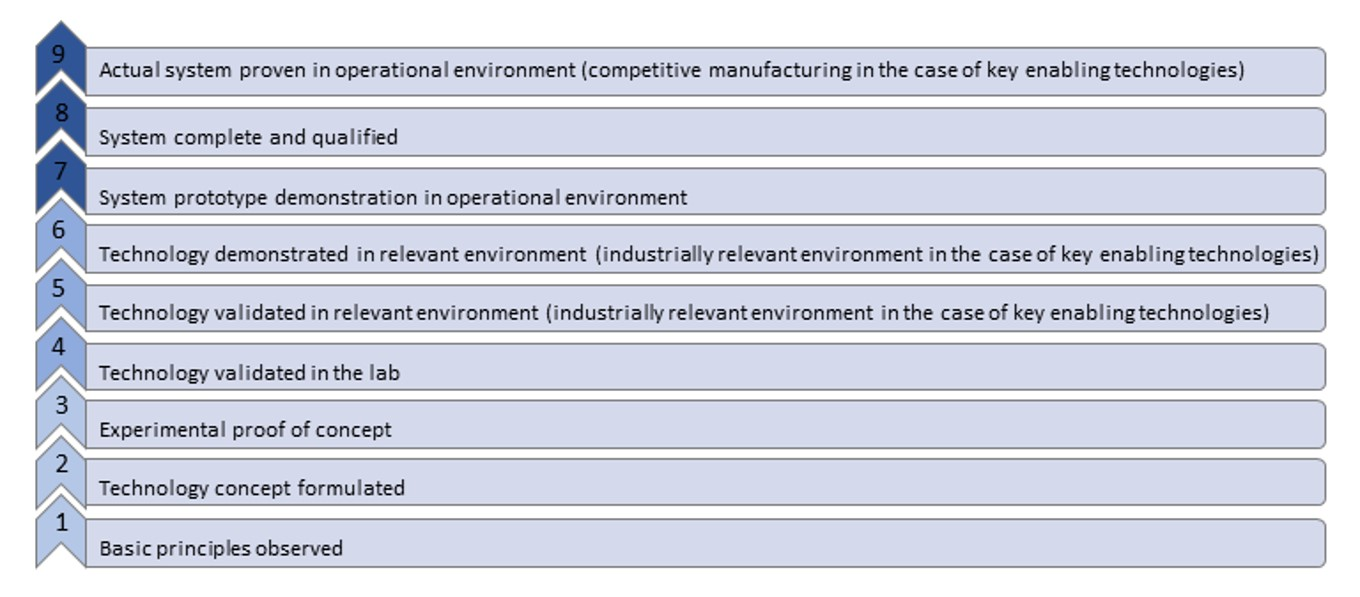
\includegraphics[width=0.6\linewidth]{image/TRL_cropped} \caption{Technology readiness scale}\label{fig:unnamed-chunk-2}
\end{figure}

Furthermore, we evaluate the readiness of a given technology to be acceptable in the society and how well it contributes to the public good using \textbf{societal readiness scale} (McCulloch, 2019):

\begin{figure}
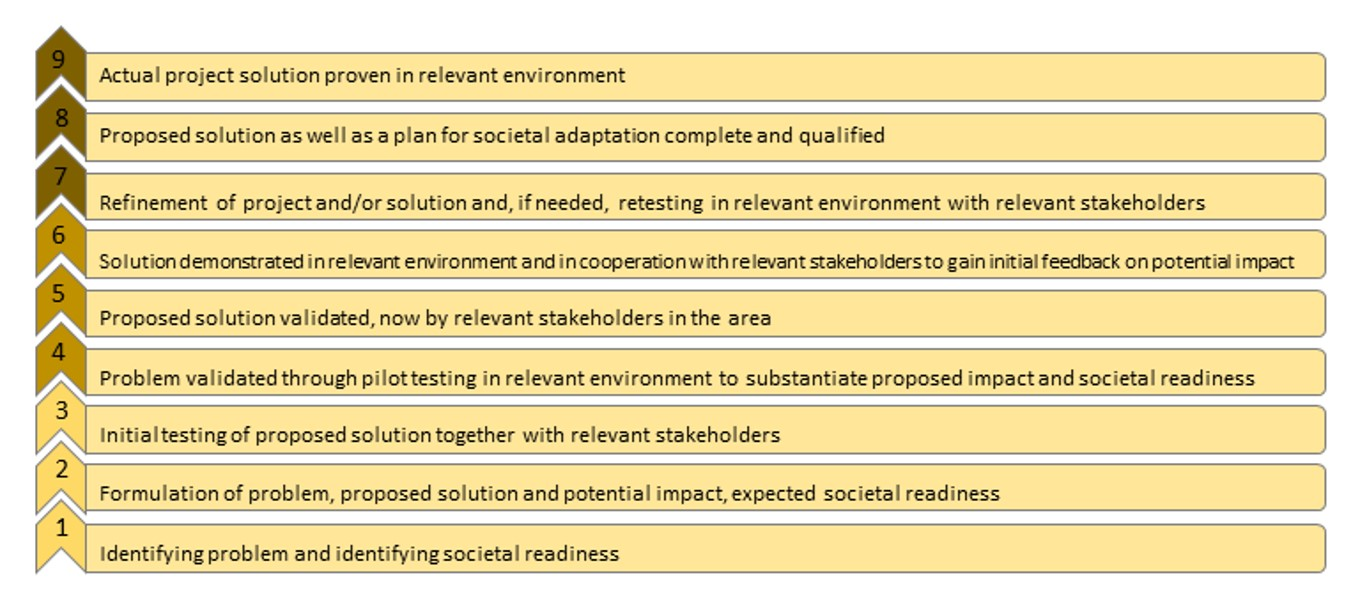
\includegraphics[width=0.6\linewidth]{image/SRL_cropped} \caption{Societal readiness scale}\label{fig:unnamed-chunk-3}
\end{figure}

Finally, we provide a list of \textbf{outstanding questions} and \textbf{links to additional sources} on the topic.

\textbf{References}

\begin{itemize}
\tightlist
\item
  Williamson, R., \& Beasley, J. (2011). \emph{Automotive technology and manufacturing readiness levels: a guide to recognised stages of development within the automotive industry}. URN11/672.
\item
  McCulloch, S. (2019). Social Acceptance And Societal Readiness Levels. {[}online{]} \emph{DecarboN8}. Available at: \url{https://decarbon8.org.uk/social-acceptance-and-societal-readiness-levels/\#:~:text=Societal\%20readiness\%20refers\%20to\%20the,contributes\%20to\%20the\%20public\%20good.} {[}Accessed 21 January 2021{]}.
\end{itemize}

\hypertarget{infrastructure}{%
\chapter{Physical road infrastructure}\label{infrastructure}}

\hypertarget{dedicated-lanes-for-connected-and-automated-vehicles-cav}{%
\section{Dedicated lanes for connected and automated vehicles (CAV)}\label{dedicated-lanes-for-connected-and-automated-vehicles-cav}}

\hypertarget{synonyms}{%
\subsection*{Synonyms}\label{synonyms}}
\addcontentsline{toc}{subsection}{Synonyms}

\emph{AV-dedicated lanes}, \emph{dedicated corridors}

\hypertarget{definition}{%
\subsection*{Definition}\label{definition}}
\addcontentsline{toc}{subsection}{Definition}

Dedicated lane for connected and autonomous vehicles features additional infrastructure or sensors to increase the reliability of Advanced Driver Assistant Systems (ADAS). Only automated driving vehicles are allowed to drive on these lanes. The typical applications include cooperative and adaptive cruise control based on sensors with the infrastructure, lane keeping, fuel use optimization and road pricing possibilities (Broek et al., 2011). The introduction of dedicated lanes for CAV is expected to have direct consequences on the traffic flow on the highways and a nearby road network. In particular, a study conducted in Singapore showed that dedicated lanes on the highways can reduce travel time of CAVs by approximately 25\% (if the saturation on the lane is not reached) at the cost of a delay for conventional cars of approximately 7\%, due to the reduced capacity (Ivanchev et al., 2017). They were also demonstrated to have a positive effect on fuel consumption.
Moreover, the throughput, defined as a number of vehicles passing through the road in a given time interval, increased as a result of introduction of dedicated lanes for AVs (Kumar et al., 2020). This effect, however, was associated with a decrease in throughput of smaller roads due to the preference of AVs for highways because of time savings, which in turn can result in time loss for conventional cars. What is more, the benefits from increased capacity of AV-only lanes can be further amplified through setting a higher speed limits for these lanes (Ye \& Yamamoto, 2018). With respect to the demand for different road types the study found that the introduction of dedicated CAV lanes will increase the demand of conventional cars for major road (but smaller than highways) and minor roads as a substitution for more congested highways due to the dedicated AV lanes.
In contrast, study by Chen et al.~(2016) showed that the implementation of CAV dedicated lanes has a potential of maximizing traffic capacity on these lanes in a mix-traffic context while having effectively no impact on conventional traffic capacity. Further, in order to use efficiently CAV dedicated lanes, which may be underutilized at the early stage, it is proposed to allow conventional cars to enter the AVs-only lanes after toll payment. This solution stems from currently operational across the world High Occupancy Vehicle (HOV) lanes. This joint approach is claimed to improve the throughput of individual road as well as enhance system-wide flow distribution within the network (Liu \& Song, 2019).

\hypertarget{key-stakeholders}{%
\subsection*{Key stakeholders}\label{key-stakeholders}}
\addcontentsline{toc}{subsection}{Key stakeholders}

\begin{itemize}
\tightlist
\item
  \textbf{Affected}: Conventional Cars' Drivers, Car Manufacturers, Insurers
\item
  \textbf{Responsible}: Road Infrastructure Agencies, Local and National Governments
\end{itemize}

\hypertarget{current-state-of-art-in-research}{%
\subsection*{Current state of art in research}\label{current-state-of-art-in-research}}
\addcontentsline{toc}{subsection}{Current state of art in research}

Current research focuses on gathering the evidence of the impact of the introduction of dedicated lanes on traffic flow, driver behavior adoption, safety and efficiency. Furthermore, it analyses the factors which influence them, by testing different design and operation configurations, road types and utilization policies (Rad et al., 2020). Both, field operational testing and driving simulator studies have been conducted to investigate the influence of different designs of dedicated lanes on drivers in conventional cars and those featuring some degree of automation (Guin et al., 2008, Zhong, 2018). In particular, a number of studies compared distinct access types of dedicated lanes (Zhong, 2018, Yang et al., 2019). They showed that dedicated lanes with limited access performed better in terms of travel time and throughput compared to dedicated lanes with continuous access. Moreover, the probability of vehicles platooning was significantly higher on dedicated lanes with limited access. On the other hand, it was showed that collision rates near the entry or exit of these limited access lanes are higher (Rad et al.~2020).

\hypertarget{current-state-of-art-in-practice}{%
\subsection*{Current state of art in practice}\label{current-state-of-art-in-practice}}
\addcontentsline{toc}{subsection}{Current state of art in practice}

Currently state of Michigan together with several private partners including Ford and Alphabet Inc.~are planning to dedicate 65 km of a highway between Detroit and Ann Arbor for the sole movement of autonomous vehicles including buses and shuttles (Krisher \& Eggert, 2020). Similar initiatives are taking place in other countries, for instance, China set out to build nearly 100 km of 8-lane highway linking Beijing and the Xiongan New Area, from which 2 lanes will be allocated for the automated traffic. The completion of the construction phase is predicted by the end of 2020, while its opening is for traffic is expected in June 2021 (Syncedreview.com, 2020). In Europe, there is on-going SHOW (SHared automation Operating models for Worldwide adoption) project which aims to deploy about seventy automated vehicles in 21 European cities. To assess how they can best be integrated vehicles will be used in different settings in mixed traffic and dedicated lanes. However, for safety reasons the driver will be on-board (CORDIS, 2020).

\hypertarget{relevant-initiatives-in-austria}{%
\subsection*{Relevant initiatives in Austria}\label{relevant-initiatives-in-austria}}
\addcontentsline{toc}{subsection}{Relevant initiatives in Austria}

\begin{itemize}
\tightlist
\item
  \href{https://www.tugraz.at/fileadmin/user_upload/Institute/IHF/Projekte/ENABLE-S3_SummaryofResults_May2019.pdf}{tugraz.at}
\item
  \href{https://www.ait.ac.at/themen/verkehrssicherheit-und-unfallforschung/projects/via-autonom/}{ait.ac.at}
\end{itemize}

\hypertarget{impacts-with-respect-to-sustainable-development-goals-sdgs}{%
\subsection*{Impacts with respect to Sustainable Development Goals (SDGs)}\label{impacts-with-respect-to-sustainable-development-goals-sdgs}}
\addcontentsline{toc}{subsection}{Impacts with respect to Sustainable Development Goals (SDGs)}

\begin{longtable}[]{@{}ccccc@{}}
\toprule
\begin{minipage}[b]{0.17\columnwidth}\centering
Impact level\strut
\end{minipage} & \begin{minipage}[b]{0.16\columnwidth}\centering
Indicator\strut
\end{minipage} & \begin{minipage}[b]{0.17\columnwidth}\centering
Impact direction\strut
\end{minipage} & \begin{minipage}[b]{0.17\columnwidth}\centering
Goal description and number\strut
\end{minipage} & \begin{minipage}[b]{0.17\columnwidth}\centering
Source\strut
\end{minipage}\tabularnewline
\midrule
\endhead
\begin{minipage}[t]{0.17\columnwidth}\centering
Individual\strut
\end{minipage} & \begin{minipage}[t]{0.16\columnwidth}\centering
Fuel consumption reduced\strut
\end{minipage} & \begin{minipage}[t]{0.17\columnwidth}\centering
\textbf{+}\strut
\end{minipage} & \begin{minipage}[t]{0.17\columnwidth}\centering
Environmental sustainability (\emph{7,12,13,15})\strut
\end{minipage} & \begin{minipage}[t]{0.17\columnwidth}\centering
Ivanchev et al., 2017\strut
\end{minipage}\tabularnewline
\begin{minipage}[t]{0.17\columnwidth}\centering
Individual\strut
\end{minipage} & \begin{minipage}[t]{0.16\columnwidth}\centering
Travel time reduced\strut
\end{minipage} & \begin{minipage}[t]{0.17\columnwidth}\centering
\textbf{+}\strut
\end{minipage} & \begin{minipage}[t]{0.17\columnwidth}\centering
Sustainable economic development (\emph{8,11})\strut
\end{minipage} & \begin{minipage}[t]{0.17\columnwidth}\centering
Zhong, 2018; Yang et al., 2019\strut
\end{minipage}\tabularnewline
\begin{minipage}[t]{0.17\columnwidth}\centering
Systemic\strut
\end{minipage} & \begin{minipage}[t]{0.16\columnwidth}\centering
Collision rate reduced\strut
\end{minipage} & \begin{minipage}[t]{0.17\columnwidth}\centering
\textbf{+}\strut
\end{minipage} & \begin{minipage}[t]{0.17\columnwidth}\centering
Health \& Wellbeing (\emph{3})\strut
\end{minipage} & \begin{minipage}[t]{0.17\columnwidth}\centering
Zhang et al., 2020\strut
\end{minipage}\tabularnewline
\begin{minipage}[t]{0.17\columnwidth}\centering
Systemic\strut
\end{minipage} & \begin{minipage}[t]{0.16\columnwidth}\centering
Emissions rate reduced\strut
\end{minipage} & \begin{minipage}[t]{0.17\columnwidth}\centering
\textbf{+}\strut
\end{minipage} & \begin{minipage}[t]{0.17\columnwidth}\centering
Environmental sustainability (\emph{7,12,13,15})\strut
\end{minipage} & \begin{minipage}[t]{0.17\columnwidth}\centering
Al Alam at al., 2010\strut
\end{minipage}\tabularnewline
\begin{minipage}[t]{0.17\columnwidth}\centering
Systemic\strut
\end{minipage} & \begin{minipage}[t]{0.16\columnwidth}\centering
Congestion\strut
\end{minipage} & \begin{minipage}[t]{0.17\columnwidth}\centering
\textbf{\textasciitilde{}}\strut
\end{minipage} & \begin{minipage}[t]{0.17\columnwidth}\centering
Sustainable economic development (\emph{8,11})\strut
\end{minipage} & \begin{minipage}[t]{0.17\columnwidth}\centering
Ivanchev et al., 2017; Kumar et al., 2020\strut
\end{minipage}\tabularnewline
\begin{minipage}[t]{0.17\columnwidth}\centering
Systemic\strut
\end{minipage} & \begin{minipage}[t]{0.16\columnwidth}\centering
Novel designs tested\strut
\end{minipage} & \begin{minipage}[t]{0.17\columnwidth}\centering
\textbf{+}\strut
\end{minipage} & \begin{minipage}[t]{0.17\columnwidth}\centering
Innovation \& Infrastructure (\emph{9})\strut
\end{minipage} & \begin{minipage}[t]{0.17\columnwidth}\centering
Guin et al., 2008; Zhong, 2018; Krisher \& Eggert, 2020\strut
\end{minipage}\tabularnewline
\begin{minipage}[t]{0.17\columnwidth}\centering
Systemic\strut
\end{minipage} & \begin{minipage}[t]{0.16\columnwidth}\centering
SHOW EU initiative\strut
\end{minipage} & \begin{minipage}[t]{0.17\columnwidth}\centering
\textbf{+}\strut
\end{minipage} & \begin{minipage}[t]{0.17\columnwidth}\centering
Partnership \& collaborations (\emph{17})\strut
\end{minipage} & \begin{minipage}[t]{0.17\columnwidth}\centering
CORDIS, 2020\strut
\end{minipage}\tabularnewline
\bottomrule
\end{longtable}

\hypertarget{technology-and-societal-readiness-level}{%
\subsection*{Technology and societal readiness level}\label{technology-and-societal-readiness-level}}
\addcontentsline{toc}{subsection}{Technology and societal readiness level}

\begin{longtable}[]{@{}cc@{}}
\toprule
TRL & SRL\tabularnewline
\midrule
\endhead
5-6 & 1-3\tabularnewline
\bottomrule
\end{longtable}

\hypertarget{open-questions}{%
\subsection*{Open questions}\label{open-questions}}
\addcontentsline{toc}{subsection}{Open questions}

\begin{enumerate}
\def\labelenumi{\arabic{enumi}.}
\tightlist
\item
  What are the potential benefits of dedicated AV lanes when coupled with smart platooning strategies?
\item
  How and to what degree will joint concepts by automotive sector, fleet and road
  operators will improve traffic management establishing dynamic traffic regulations even across
  borders?
\item
  What are the roles and responsibilities of the different stakeholders of physical infrastructure for connected and automated vehicles?
\item
  Should the vehicle cope with any road infrastructure, and if not, what demands can be set to adapt the existing infrastructure?
\item
  How to ensure continuity between those different environments?
\item
  Which tools (e.g.~micro- and macroscopic transport modelling, impact assessment) can enable
  cities to assess the impact of automated vehicles on their physical road infrastructure and
  balance the needs of automated vehicles against the needs of existing modes (conventional
  vehicles, public transport, pedestrians and cyclists). (ERTRAC, 2019)
\end{enumerate}

\hypertarget{further-links}{%
\subsection*{Further links}\label{further-links}}
\addcontentsline{toc}{subsection}{Further links}

\begin{itemize}
\tightlist
\item
  \href{https://knowledge-base.connectedautomateddriving.eu/wp-content/uploads/2019/12/SMART_2010-0064-study-report-final_V1-2.pdf}{knowledge base}
\item
  \href{https://show-project.eu/}{show project}
\end{itemize}

\hypertarget{references}{%
\subsection*{References}\label{references}}
\addcontentsline{toc}{subsection}{References}

\begin{itemize}
\tightlist
\item
  Al Alam, A., Gattami, A., \& Johansson, K. H. (2010, September). An experimental study on the fuel reduction potential of heavy duty vehicle platooning. In 13th International IEEE Conference on Intelligent Transportation Systems (pp.~306-311). IEEE.
  Broek, S. M., van Nunen, E., \& Zwijnenberg, H. (2011). Definition of necessary vehicle and infrastructure systems for automated driving. Retrieved January, 3, 2017.
\item
  Chen, Z., He, F., Zhang, L., \& Yin, Y. (2016). Optimal deployment of autonomous vehicle lanes with endogenous market penetration. Transportation Research Part C: Emerging Technologies, 72, 143-156.
\item
  CORDIS \textbar{} European Commission. (20 Apr 2020). Retrieved 13 November 2020, from \url{https://cordis.europa.eu/project/id/875530}
\item
  ERTRAC Working Group. (2019). Connected Automated Driving Roadmap. version, 8, 2019-08.
\item
  Guin, A., Hunter, M., \& Guensler, R. (2008). Analysis of reduction in effective capacities of high-occupancy vehicle lanes related to traffic behavior. Transportation Research Record, 2065(1), 47-53.
\item
  Ivanchev, J., Knoll, A., Zehe, D., Nair, S., \& Eckhoff, D. (2017). Potentials and implications of dedicated highway lanes for autonomous vehicles. arXiv preprint arXiv:1709.07658.
\item
  Krisher, T., \& Eggert, D. (14 Aug 2020). Michigan plans dedicated road lanes for autonomous vehicles. Retrieved 12 November 2020, from \url{https://abcnews.go.com/Technology/wireStory/michigan-plans-dedicated-road-lanes-autonomous-vehicles-72352758}
\item
  Kumar, A., Guhathakurta, S., \& Venkatachalam, S. (2020). When and where should there be dedicated lanes under mixed traffic of automated and human-driven vehicles for system-level benefits?. Research in Transportation Business \& Management, 100527.
\item
  Liu, Z., \& Song, Z. (2019). Strategic planning of dedicated autonomous vehicle lanes and autonomous vehicle/toll lanes in transportation networks. Transportation Research Part C: Emerging Technologies, 106, 381-403.
\item
  Rad, S. R., Farah, H., Taale, H., van Arem, B., \& Hoogendoorn, S. P. (2020). Design and operation of dedicated lanes for connected and automated vehicles on motorways: A conceptual framework and research agenda. Transportation Research Part C: Emerging Technologies, 117, 102664.
\item
  Syncedreview.com (31 Aug 2020). Beijing Builds 100km Highway Lanes for Self-Driving Cars with Unmanned Machineries. Retrieved 12 November 2020, from \url{https://syncedreview.com/2020/08/31/beijing-builds-100km-highway-lanes-for-self-driving-cars-with-unmanned-machineries/}
\item
  Yang, D., Farah, H., Schoenmakers, M. J., \& Alkim, T. (2019). Human drivers behavioural adaptation when driving next to a platoon of automated vehicles on a dedicated lane and implications on traffic flow: a driving simulator and microscopic simulation study in the Netherlands. In 98th Annual Meeting of the Transportation Research Board (pp.~19-00582).
\item
  Ye, L., \& Yamamoto, T. (2018). Impact of dedicated lanes for connected and autonomous vehicle on traffic flow throughput. Physica A: Statistical Mechanics and its Applications, 512, 588-597.
\item
  Zhang, J., Wu, K., Cheng, M., Yang, M., Cheng, Y., \& Li, S. (2020). Safety Evaluation for Connected and Autonomous Vehicles' Exclusive Lanes considering Penetrate Ratios and Impact of Trucks Using Surrogate Safety Measures. Journal of advanced transportation, 2020.
\item
  Zhong, Z. (2018). Assessing the effectiveness of managed lane strategies for the rapid deployment of cooperative adaptive cruise control technology.
\end{itemize}

\hypertarget{cooperative-lane-control-for-connected-and-automated-vehicles}{%
\section{Cooperative lane control for connected and automated vehicles}\label{cooperative-lane-control-for-connected-and-automated-vehicles}}

\hypertarget{operational-design-domains}{%
\section{Operational design domains}\label{operational-design-domains}}

\hypertarget{rail-crossing-information-system}{%
\section{Rail crossing information system}\label{rail-crossing-information-system}}

\hypertarget{electric-road-system}{%
\section{Electric road system}\label{electric-road-system}}

\hypertarget{high-occupancy-toll-lanes}{%
\section{High occupancy toll lanes}\label{high-occupancy-toll-lanes}}

\hypertarget{public-transport-priority-systems}{%
\section{Public transport priority systems}\label{public-transport-priority-systems}}

\hypertarget{synonyms-1}{%
\subsection*{Synonyms}\label{synonyms-1}}
\addcontentsline{toc}{subsection}{Synonyms}

\emph{pre-emption of public transport vehicles, public transport priority (PTP), Transit signal priority (TSP), road-space priority (RSP)}

\hypertarget{definition-1}{%
\subsection*{Definition}\label{definition-1}}
\addcontentsline{toc}{subsection}{Definition}

To encourage people to use public transport and thereby travel more sustainably, it is necessary that public transport operates reliably and efficiently. For example, public transport is the most efficient mode of transport at the intersections, where the difference in the number of people who can pass through a junction in a given time is particularly impressive between cars and public transport. The ratio is between 1 to 10 and 1 to 20 (Schwendinger, 2019). In contrast, a bus at full capacity that is stuck in congestion increases the travel time of many more passengers, compared to single cars in a similar position. Time delays due to traffic signals account for up to 25\% of the total travel time of buses (Seredynski et al., 2015). Furthermore, energy prices and emissions generated become more relevant for public transport operators, to compete with the motorized private transport (Gassel et al., 2012).
The implementation of public transport priority measures can help improving time and energy efficiency of public transport service. The delays caused by traffic signals can be reduced by the introduction of Transit Signal Priority (TSP) such as early green, green extension, phase rotation, phase insertion and actuated transit phase, favouring public transport (Seredynski et al., 2015). TSP systems can increase the attractiveness of public transport, reduce the operation cost and reduce tailpipe emissions and energy use. On the other hand, they increase the travel time of general traffic, therefore the acceptance is limited (Seredynski et al., 2015). Another widely used systems are separated bus lanes or independent tracks for trams. These are especially relevant in 30 km/h zones, so the public transport vehicles can be excluded from the regulation. But since space is a limited good, independent lanes or tracks are not always possible to implement (Schwendinger, 2019).
For Vienna priority of public transport vehicles is of high importance (WIENER STADTWERKE GmbH, 2018). The first measures to shorten the travel time of the bus route 15A at Wienerberg took effect in Autumn 2018. Measures to give priority to public transport are also becoming more important in other cities such as Linz, Graz or Innsbruck. Trams in Graz have priority switching at almost all traffic lights, while there is a further need for bus lines, especially for those from the surrounding area (Schwendinger, 2019).To promote e-mobility, some countries introduced bus lane access to e-vehicles (Figenbaum et al., 2015). Wiener Linien is clearly against this measure, because cars, regardless of their propulsion system, cause delays in the bus lanes and slow down public transport (WIENER STADTWERKE GmbH, 2018).

\hypertarget{key-stakeholders-1}{%
\subsection*{Key stakeholders}\label{key-stakeholders-1}}
\addcontentsline{toc}{subsection}{Key stakeholders}

\begin{itemize}
\tightlist
\item
  \textbf{Affected}: Road Users, Public Transport Users, Public Transport Operators
\item
  \textbf{Responsible}: State Authorities, Transport Infrastructure Operators, Technology Providers
\end{itemize}

\hypertarget{current-state-of-art-in-research-1}{%
\subsection*{Current state of art in research}\label{current-state-of-art-in-research-1}}
\addcontentsline{toc}{subsection}{Current state of art in research}

Current research aims at building on the existing solutions such as TSP and proposes so-called Green Light Optimal Speed Advisory (GLOSA) driver assistance systems. A multi segment GLOSA can take several lights in a sequence on route of a bus into account and allows the driver to adjust the speed, so that the bus can arrive at the intersection when the light is green. By that, the comfort of passengers can be increased and the fuel consumption as well as the tailpipe emissions be decreased, without negatively affecting the general traffic (Seredynski et al., 2014). However, Stahlmann et al.~(2018) argue that so far, most GLOSA simulation studies are too optimistic in terms of communication performance and recommend further improvement of GLOSA systems.
Moreover, the Green Light Optimal Dwell Time Advisory (GLODTA) systems look into exploiting additional dwell time at the near-side bus stop (Seredynski et al., 2014). According to Seredynski \& Viti (2017) they can support on-route battery charging of electrical buses and also replace existing holding strategies used to regulate punctuality of bus services.
Due the limited acceptance of TSP systems, more research regarding the efficient use of green time provided to public transport is needed. Therefore, the focus is on the improvement of the bus detection methods. The latest TSP are working with GPS-based Virtual Detectors (VD), which eliminate the need of on-street detection infrastructure, but their disadvantages is low accuracy (Seredynski et al., 2015).
Haitao et al.~(2019) developed an integrated and systematic framework for the optimization of bimodal urban networks using 3D-MFDs, considering the complexities of bimodality to manage traffic more efficiently and provide public transport priority. Results of the evaluation show that the proposed strategy always performs better than existing perimeter control schemes in terms of passenger mobility.

\hypertarget{current-state-of-art-in-practice-1}{%
\subsection*{Current state of art in practice}\label{current-state-of-art-in-practice-1}}
\addcontentsline{toc}{subsection}{Current state of art in practice}

A common measure in use is the positioning of stops before intersections, which combines the standing time at the traffic lights with the passenger change and thus leads to travel time reductions (Schwendinger, 2019).
All around the world Bus Rapid Transit (BRT) systems have gained popularity. Cervero (2013) defines them as ``bus-based system that mimics the high-capacity, high-performance characteristics of urban rail systems at a much lower price'' that runs either on exclusive transit-ways, dedicated bus lanes or some grade of separation.
Regarding TPS, the cloud-based systems using GPS locations are standard technology (see Figure 1). However, there are still many outdated systems in use that are based on short-range radio. These systems require that all traffic lights are equipped with receivers. All buses in a fleet need special transmitters and an onboard system for positioning, which makes it an overall expensive system. At the same time, this technology is rather unreliable and maintenance intensive (SWARCO, 2021).

\begin{figure}
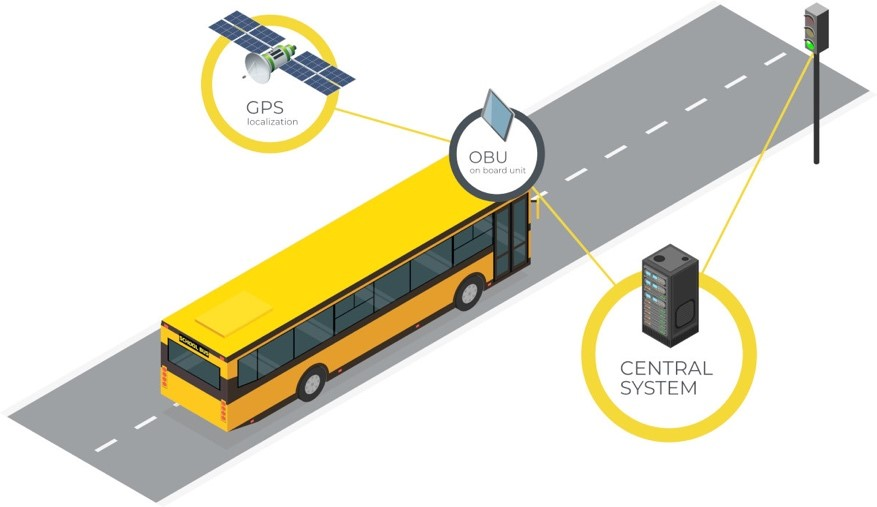
\includegraphics[width=0.7\linewidth]{image/pt_priority_system} \caption{Smart priority for public transport (SWARCO, 2021)}\label{fig:unnamed-chunk-4}
\end{figure}

\hypertarget{relevant-initiatives-in-austria-1}{%
\subsection*{Relevant initiatives in Austria}\label{relevant-initiatives-in-austria-1}}
\addcontentsline{toc}{subsection}{Relevant initiatives in Austria}

\begin{itemize}
\tightlist
\item
  \href{https://digitales.wien.gv.at/site/open-data/}{digitales.wien.gv.at}
\item
  \href{https://www.wienerlinien.at/eportal3/ep/channelView.do/pageTypeId/66528/channelId/-4400661}{wienerlinien.at}
\item
  \href{https://www.kapsch.net/ktc/Portfolio/IMS/Congestion/Managed-lanes}{kapsch.net-1}
\item
  \href{https://www.kapsch.net/ktc/Portfolio/IMS/Smart-Urban-Mobility/Urban-Mobility-Management}{kapsch.net-2}
\item
  \href{https://www.swarco.com/de/loesungen/oeffentlicher-nahverkehr/vorrang-fuer-den-oeffentlichen-nahverkehr}{swarco.com}
\item
  \href{https://www.mobility.siemens.com/global/de/portfolio/strasse/verkehrsmanagement/auf-der-strasse/smart-detection.html}{mobility.siemens.com}
\end{itemize}

\hypertarget{impacts-with-respect-to-sustainable-development-goals-sdgs-1}{%
\subsection*{Impacts with respect to Sustainable Development Goals (SDGs)}\label{impacts-with-respect-to-sustainable-development-goals-sdgs-1}}
\addcontentsline{toc}{subsection}{Impacts with respect to Sustainable Development Goals (SDGs)}

\begin{longtable}[]{@{}ccccc@{}}
\toprule
\begin{minipage}[b]{0.17\columnwidth}\centering
Impact level\strut
\end{minipage} & \begin{minipage}[b]{0.16\columnwidth}\centering
Indicator\strut
\end{minipage} & \begin{minipage}[b]{0.17\columnwidth}\centering
Impact direction\strut
\end{minipage} & \begin{minipage}[b]{0.17\columnwidth}\centering
Goal description and number\strut
\end{minipage} & \begin{minipage}[b]{0.17\columnwidth}\centering
Source\strut
\end{minipage}\tabularnewline
\midrule
\endhead
\begin{minipage}[t]{0.17\columnwidth}\centering
Individual\strut
\end{minipage} & \begin{minipage}[t]{0.16\columnwidth}\centering
Higher equality for people who do not drive\strut
\end{minipage} & \begin{minipage}[t]{0.17\columnwidth}\centering
\textbf{+}\strut
\end{minipage} & \begin{minipage}[t]{0.17\columnwidth}\centering
Equality (\emph{5,10})\strut
\end{minipage} & \begin{minipage}[t]{0.17\columnwidth}\centering
Litman, 2017; Cervero, 2013\strut
\end{minipage}\tabularnewline
\begin{minipage}[t]{0.17\columnwidth}\centering
Individual\strut
\end{minipage} & \begin{minipage}[t]{0.16\columnwidth}\centering
Less travel time for public transport users, more travel time for car users\strut
\end{minipage} & \begin{minipage}[t]{0.17\columnwidth}\centering
\textbf{\textasciitilde{}}\strut
\end{minipage} & \begin{minipage}[t]{0.17\columnwidth}\centering
Sustainable economic development (\emph{8,11})\strut
\end{minipage} & \begin{minipage}[t]{0.17\columnwidth}\centering
Seredynski et al., 2015\strut
\end{minipage}\tabularnewline
\begin{minipage}[t]{0.17\columnwidth}\centering
Systemic\strut
\end{minipage} & \begin{minipage}[t]{0.16\columnwidth}\centering
Public transport becomes more competitive compared to other transport modes\strut
\end{minipage} & \begin{minipage}[t]{0.17\columnwidth}\centering
\textbf{+}\strut
\end{minipage} & \begin{minipage}[t]{0.17\columnwidth}\centering
Equality (\emph{5,10})\strut
\end{minipage} & \begin{minipage}[t]{0.17\columnwidth}\centering
Schwendinger, 2019\strut
\end{minipage}\tabularnewline
\begin{minipage}[t]{0.17\columnwidth}\centering
Systemic\strut
\end{minipage} & \begin{minipage}[t]{0.16\columnwidth}\centering
Less fuel consumption\strut
\end{minipage} & \begin{minipage}[t]{0.17\columnwidth}\centering
\textbf{+}\strut
\end{minipage} & \begin{minipage}[t]{0.17\columnwidth}\centering
Environmental sustainability (\emph{7,12,13,15})\strut
\end{minipage} & \begin{minipage}[t]{0.17\columnwidth}\centering
Gassel et al., 2012; Seredynski et al., 2015\strut
\end{minipage}\tabularnewline
\begin{minipage}[t]{0.17\columnwidth}\centering
Systemic\strut
\end{minipage} & \begin{minipage}[t]{0.16\columnwidth}\centering
Transit is often the most cost-effective mode\strut
\end{minipage} & \begin{minipage}[t]{0.17\columnwidth}\centering
\textbf{+}\strut
\end{minipage} & \begin{minipage}[t]{0.17\columnwidth}\centering
Sustainable economic development (\emph{8,11})\strut
\end{minipage} & \begin{minipage}[t]{0.17\columnwidth}\centering
Litman, 2015\strut
\end{minipage}\tabularnewline
\begin{minipage}[t]{0.17\columnwidth}\centering
Systemic\strut
\end{minipage} & \begin{minipage}[t]{0.16\columnwidth}\centering
More infrastructre for public transport\strut
\end{minipage} & \begin{minipage}[t]{0.17\columnwidth}\centering
\textbf{+}\strut
\end{minipage} & \begin{minipage}[t]{0.17\columnwidth}\centering
Innovation \& Infrastructure (\emph{9})\strut
\end{minipage} & \begin{minipage}[t]{0.17\columnwidth}\centering
Cuthill et al., 2019\strut
\end{minipage}\tabularnewline
\bottomrule
\end{longtable}

\hypertarget{technology-and-societal-readiness-level-1}{%
\subsection*{Technology and societal readiness level}\label{technology-and-societal-readiness-level-1}}
\addcontentsline{toc}{subsection}{Technology and societal readiness level}

\begin{longtable}[]{@{}cc@{}}
\toprule
TRL & SRL\tabularnewline
\midrule
\endhead
4-8 & 5-8\tabularnewline
\bottomrule
\end{longtable}

\hypertarget{open-questions-1}{%
\subsection*{Open questions}\label{open-questions-1}}
\addcontentsline{toc}{subsection}{Open questions}

\begin{enumerate}
\def\labelenumi{\arabic{enumi}.}
\tightlist
\item
  Who is responsible for the implementation of PTP systems?
\item
  How will Vehicle-to-Vehicle (V2V), Vehicle-to-Infrastructure (V2I) and in future Vehicle-to-Pedestrian (V2P) change PTP systems?
\item
  How could also emergency vehicles be prioritised?
\item
  How to deal with mixed fleets - half new, half old?
\item
  What are the benefits compared to the costs?
\item
  Which standards should be used?
\end{enumerate}

\hypertarget{references-1}{%
\subsection*{References}\label{references-1}}
\addcontentsline{toc}{subsection}{References}

\begin{itemize}
\tightlist
\item
  Cervero, R. (2013). Bus rapid transit (BRT): An efficient and competitive mode of public transport (No.~2013-01). Working Paper.
\item
  Cuthill, N., Cao, M., Liu, Y., Gao, X., \& Zhang, Y. (2019). The association between urban public transport infrastructure and social equity and spatial accessibility within the urban environment: An investigation of Tramlink in London. Sustainability, 11(5), 1229.
\item
  Figenbaum, E., Fearnley, N., Pfaffenbichler, P., Hjorthol, R., Kolbenstvedt, M., Jellinek, R., \ldots{} \& Iversen, L. M. (2015). Increasing the competitiveness of e-vehicles in Europe. European transport research review, 7(3), 1-14.
\item
  Gassel, C., Matschek, T., \& Krimmling, J. (2012). Cooperative traffic signals for energy efficient driving in tramway systems. Aspekte der Verkehrstelematik--ausgewählte Veröffentlichungen 2012, 1.
\item
  Haitao, H., Yang, K., Liang, H., Menendez, M., \& Guler, S. I. (2019). Providing public transport priority in the perimeter of urban networks: A bimodal strategy. Transportation Research Part C: Emerging Technologies, 107, 171-192.
\item
  Litman, T. (2015). Evaluating public transit benefits and costs. Victoria, BC, Canada: Victoria Transport Policy Institute.
\item
  Litman, T. (2017). Evaluating Transportation Diversity. Victoria Transport Policy Institute.
\item
  Schwendinger, M. (2019). Vorrang für Busse und Straßenbahnen in Städten. \url{https://vcoe.at/files/vcoe/uploads/Projekte/Factsheets} 2019 Neu/VCÖ-Factsheet ÖV-Bevorrangen.pdf
\item
  Seredynski, M., Khadraoui, D., \& Viti, F. (2015, October). Signal phase and timing (SPaT) for cooperative public transport priority measures. In Proc. 22nd ITS World Congress.
\item
  Seredynski, M., Ruiz, P., Szczypiorski, K., \& Khadraoui, D. (2014, May). Improving bus ride comfort using GLOSA-based dynamic speed optimisation. In 2014 IEEE International Parallel \& Distributed Processing Symposium Workshops (pp.~457-463). IEEE.
\item
  Seredynski, M., \& Viti, F. (2017, October). Novel C-ITS support for electric buses with opportunity charging. In 2017 IEEE 20th International Conference on Intelligent Transportation Systems (ITSC) (pp.~1-6). IEEE.
\item
  Stahlmann, R., Möller, M., Brauer, A., German, R., \& Eckhoff, D. (2018). Exploring GLOSA systems in the field: Technical evaluation and results. Computer Communications, 120, 112-124.
\item
  SWARCO. (2021). Vorrang für den ÖPNV: Öffentliche Verkehrsmittel attraktiver machen. Retrieved 26th January 2021, from \url{https://www.swarco.com/de/loesungen/oeffentlicher-nahverkehr/vorrang-fuer-den-oeffentlichen-nahverkehr}
\item
  WIENER STADTWERKE GmbH. (2018). Wiener Linien: Autos auf Busspuren halten Öffis auf. \url{https://www.wienerstadtwerke.at/eportal3/ep/contentView.do?pageTypeId=71954\&channelId=-51313\&programId=72863\&contentId=4202309\&contentTypeId=1001}
\end{itemize}

\hypertarget{transformation-of-public-space-and-digital-solutions}{%
\section{Transformation of public space and digital solutions}\label{transformation-of-public-space-and-digital-solutions}}

\hypertarget{highway}{%
\chapter{Highway infrastructure management}\label{highway}}

\hypertarget{unmanned-aerial-vehicles-for-infrastructure-maintenance}{%
\section{Unmanned aerial vehicles for infrastructure maintenance}\label{unmanned-aerial-vehicles-for-infrastructure-maintenance}}

\hypertarget{synonyms-2}{%
\subsection*{Synonyms}\label{synonyms-2}}
\addcontentsline{toc}{subsection}{Synonyms}

\emph{Drones, remotely piloted vehicles, remotely piloted aircraft, uav}

\hypertarget{definition-2}{%
\subsection*{Definition}\label{definition-2}}
\addcontentsline{toc}{subsection}{Definition}

Unmanned Aerial Vehicles (UAVs), commonly known as drones are promising technologies that can be used in inspection and data gathering for infrastructure maintenance and management purposes. These include, for example, detection of wear and tear, monitoring of the progress at a highway construction site or the analysis of traffic (Frederiksen et al., 2019). UAVs typically include a portable control station for the human operator and under current legislation their operation in urban areas is limited to flying within visual line of sight (VLOS). UAVs typically feature various sensors and recorders, including video, far and near infrared, radar or laser-based range finders and specialized communication devices (Shaghlil \& Khalafallah, 2018). Majority of them can transfer real-time data between the UAV and the control station. Moreover, some feature additional onboard data storage capabilities for enhanced data collection (Shaghlil \& Khalafallah, 2018). The use of drones for infrastructure-related tasks provide not only savings with respect to time, labor and costs, but they also allow for reduction in risks when dangerous operations usually performed by human can be substituted with drones. Finally, the environmental impact is diminished when drones, which produce considerably less CO2, are used instead of currently employed helicopters. Nevertheless, the use of drones as a tool for inspecting infrastructure can also pose certain challenges with respect to current technology, legal framework, privacy concerns and social acceptance.

\hypertarget{key-stakeholders-2}{%
\subsection*{Key stakeholders}\label{key-stakeholders-2}}
\addcontentsline{toc}{subsection}{Key stakeholders}

\begin{itemize}
\tightlist
\item
  \textbf{Affected}: Direct users of the roads and beneficiaries affected by the supply of transport services
\item
  \textbf{Responsible}: Government agencies responsible for planning, executing, and financing of maintenance activities, citizens, contractors and subcontractors, private companies and manufacturers
\end{itemize}

\hypertarget{current-state-of-art-in-research-2}{%
\subsection*{Current state of art in research}\label{current-state-of-art-in-research-2}}
\addcontentsline{toc}{subsection}{Current state of art in research}

Current research efforts and field trials-based studies are advocating the case of using UAVs for bridge inspection and monitoring. Previous study presented a proof of concept of utilising UAVs for bridge and high mast luminaires. Several experiments in controlled conditions were performed to test UAV response in relation to wind conditions. Moreover, image quality was examined in different flight scenarios, low light conditions, altitude and payload (Otero et al., 2015). Overall, the results are in favour of using drones for infrastructure inspections, not just in terms of saving human labor but also detecting the damages. The advantages of the drone use were also demonstrated in terms of reduced traffic control and decreased use of under bridge inspection vehicles (Zink and Lovelace, 2015). On the other hand, specific skills of the drone operators were found to hinder efficient use of drones for large-scale bridges (Wu et al., 2018). Further, some technological barriers also slow down the popularity of drones in infrastructure inspection, where an average flight time of the drone given its battery life is approximately 30 minutes. Therefore, current research aims at increasing the energy-efficiency by the use of path planning and algorithms to minimize energy utilization while maximizing coverage for traffic monitoring (Outay et al., 2020).

\hypertarget{current-state-of-art-in-practice-2}{%
\subsection*{Current state of art in practice}\label{current-state-of-art-in-practice-2}}
\addcontentsline{toc}{subsection}{Current state of art in practice}

Current use of drones is heavily regulated by national and international governments worldwide where the most considerable restriction is the requirement for drones to remain under VLOS of the controller. Beyond, the regulatory bodies put forward various specification with respect to physical aspects of the drones such as weight or sensors, training requirement of the operators and drones', data acquisition regulations and operation itself such as flight timeframe, altitude etc. (FAA, 2016; Outay at al., 2020). All of them, significantly restrict fast and wide application of drones in different areas. Therefore, the authorities attempt to provide regulations to tackle safety and privacy as well as noise concerns of the citizens. At the moment drones are used in oil and gas industry to conduct local surveys in off-shore facilities (Undertaking, 2016). Meanwhile in the transport sector, Danish company Dronops, after safety clearance, has been granted permission from Danish Road Authority to fly along a highway to monitor the traffic, where drone provides data from multiple sensors as well as video recordings. At the moment, the drone can only fly in good weather conditions and it is cable-linked to its power source located on the ground to allow for continuous day-long monitoring at 120 m above the ground. Importantly, the output data is used by Danish Road Authority and local council (Frederiksen et al., 2019).

\hypertarget{relevant-initiatives-in-austria-2}{%
\subsection*{Relevant initiatives in Austria}\label{relevant-initiatives-in-austria-2}}
\addcontentsline{toc}{subsection}{Relevant initiatives in Austria}

\begin{itemize}
\tightlist
\item
  \href{https://smartcity.wien.gv.at/site/en/smart-inspection/}{smartcity.wien}
\end{itemize}

\hypertarget{impacts-with-respect-to-sustainable-development-goals-sdgs-2}{%
\subsection*{Impacts with respect to Sustainable Development Goals (SDGs)}\label{impacts-with-respect-to-sustainable-development-goals-sdgs-2}}
\addcontentsline{toc}{subsection}{Impacts with respect to Sustainable Development Goals (SDGs)}

\begin{longtable}[]{@{}ccccc@{}}
\toprule
\begin{minipage}[b]{0.17\columnwidth}\centering
Impact level\strut
\end{minipage} & \begin{minipage}[b]{0.16\columnwidth}\centering
Indicator\strut
\end{minipage} & \begin{minipage}[b]{0.17\columnwidth}\centering
Impact direction\strut
\end{minipage} & \begin{minipage}[b]{0.17\columnwidth}\centering
Goal description and number\strut
\end{minipage} & \begin{minipage}[b]{0.17\columnwidth}\centering
Source\strut
\end{minipage}\tabularnewline
\midrule
\endhead
\begin{minipage}[t]{0.17\columnwidth}\centering
Individual\strut
\end{minipage} & \begin{minipage}[t]{0.16\columnwidth}\centering
Employees risk reduced\strut
\end{minipage} & \begin{minipage}[t]{0.17\columnwidth}\centering
\textbf{+}\strut
\end{minipage} & \begin{minipage}[t]{0.17\columnwidth}\centering
Health \& Wellbeing (\emph{3})\strut
\end{minipage} & \begin{minipage}[t]{0.17\columnwidth}\centering
Outay et al., 2020\strut
\end{minipage}\tabularnewline
\begin{minipage}[t]{0.17\columnwidth}\centering
Systemic\strut
\end{minipage} & \begin{minipage}[t]{0.16\columnwidth}\centering
Road safety increased\strut
\end{minipage} & \begin{minipage}[t]{0.17\columnwidth}\centering
\textbf{+}\strut
\end{minipage} & \begin{minipage}[t]{0.17\columnwidth}\centering
Health \& Wellbeing (\emph{3})\strut
\end{minipage} & \begin{minipage}[t]{0.17\columnwidth}\centering
Outay et al., 2020\strut
\end{minipage}\tabularnewline
\begin{minipage}[t]{0.17\columnwidth}\centering
Systemic\strut
\end{minipage} & \begin{minipage}[t]{0.16\columnwidth}\centering
Emissions rate reduced\strut
\end{minipage} & \begin{minipage}[t]{0.17\columnwidth}\centering
\textbf{+}\strut
\end{minipage} & \begin{minipage}[t]{0.17\columnwidth}\centering
Environmental sustainability (\emph{7,12,13,15})\strut
\end{minipage} & \begin{minipage}[t]{0.17\columnwidth}\centering
Outay et al., 2020\strut
\end{minipage}\tabularnewline
\begin{minipage}[t]{0.17\columnwidth}\centering
Systemic\strut
\end{minipage} & \begin{minipage}[t]{0.16\columnwidth}\centering
Job posts created\strut
\end{minipage} & \begin{minipage}[t]{0.17\columnwidth}\centering
\textbf{+}\strut
\end{minipage} & \begin{minipage}[t]{0.17\columnwidth}\centering
Sustainable economic development (\emph{8,11})\strut
\end{minipage} & \begin{minipage}[t]{0.17\columnwidth}\centering
Jenkins \& Vasigh, 2013\strut
\end{minipage}\tabularnewline
\begin{minipage}[t]{0.17\columnwidth}\centering
Systemic\strut
\end{minipage} & \begin{minipage}[t]{0.16\columnwidth}\centering
Faster road infrastructure innovation\strut
\end{minipage} & \begin{minipage}[t]{0.17\columnwidth}\centering
\textbf{+}\strut
\end{minipage} & \begin{minipage}[t]{0.17\columnwidth}\centering
Innovation \& Infrastructure (\emph{9})\strut
\end{minipage} & \begin{minipage}[t]{0.17\columnwidth}\centering
Fan \& Saadeghvaziri, 2019\strut
\end{minipage}\tabularnewline
\bottomrule
\end{longtable}

\hypertarget{technology-and-societal-readiness-level-2}{%
\subsection*{Technology and societal readiness level}\label{technology-and-societal-readiness-level-2}}
\addcontentsline{toc}{subsection}{Technology and societal readiness level}

\begin{longtable}[]{@{}cc@{}}
\toprule
TRL & SRL\tabularnewline
\midrule
\endhead
3-4 & 5-7\tabularnewline
\bottomrule
\end{longtable}

\hypertarget{open-questions-2}{%
\subsection*{Open questions}\label{open-questions-2}}
\addcontentsline{toc}{subsection}{Open questions}

\begin{enumerate}
\def\labelenumi{\arabic{enumi}.}
\tightlist
\item
  What are the factors influencing social acceptability of drones?
\item
  What actions from the policymakers need to be undertaken to minimalize cyber-attacks?
\item
  What aspects need to be considered by the governments before the integration of more sensors to record other relevant data along with the integration of video data with other geospatial information?
\end{enumerate}

\hypertarget{further-links-1}{%
\subsection*{Further links}\label{further-links-1}}
\addcontentsline{toc}{subsection}{Further links}

\begin{itemize}
\tightlist
\item
  \href{https://www.rolandberger.com/en/Insights/Publications/Drones-The-future-of-asset-inspection.html}{rolandberger}
\end{itemize}

\hypertarget{references-2}{%
\subsection*{References}\label{references-2}}
\addcontentsline{toc}{subsection}{References}

\begin{itemize}
\tightlist
\item
  FAA News, 2016, Summary of Small Unmanned Aircraft Rule (Part 107), Federal Aviation Authority, Washington DC, 20591, Accessed on May 2020, \url{https://www.faa.gov/uas/media/Part_107_Summary.pdf}.
\item
  Fan, J., \& Saadeghvaziri, M. A. (2019). Applications of Drones in Infrastructures: Challenges and Opportunities. International Journal of Mechanical and Mechatronics Engineering, 13(10), 649-655.
\item
  Frederiksen, M. H., Mouridsen, O. A. V., \& Knudsen, M. P. (2019). Drones for inspection of infrastructure: Barriers, opportunities and successful uses.
\item
  Jenkins, D., \& Vasigh, B. (2013). The economic impact of unmanned aircraft systems integration in the United States. Association for Unmanned Vehicle Systems International (AUVSI).
\item
  Otero, L.D., Gagliardo, N., Dalli, D., Huang, W.-H., Cosentino, P. (2015). Proof of concept for using unmanned aerial vehicles for high mast pole and bridge inspections (No.~BDV28-977-02). Florida. Dept. of Transportation. Research Center.
\item
  utay, F., Mengash, H. A., \& Adnan, M. (2020). Applications of unmanned aerial vehicle (UAV) in road safety, traffic and highway infrastructure management: Recent advances and challenges. Transportation research. Part A, Policy and practice, 141, 116--129. \url{https://doi.org/10.1016/j.tra.2020.09.018}
\item
  Shaghlil, N., \& Khalafallah, A. (2018). Automating highway infrastructure maintenance using unmanned aerial vehicles. In Construction Research Congress (2-4).
\item
  Undertaking, S. J. (2016). European drones outlook study. Unlocking the Value for Europe.
\item
  Wu, W., Qurishee, M. A., Owino, J., Fomunung, I., Onyango, M., Atolagbe, B. (2018). Coupling deep learning and UAV for infrastructure condition assessment automation. In: 2018 IEEE International Smart Cities Conference (ISC2). IEEE, pp.~1--7.
\item
  Zink, J. and Lovelace, B., 2015. Unmanned aerial vehicle bridge inspection demonstration project. Research Project. Final Report, 40. Accessed in Nov 2020
\end{itemize}

\hypertarget{electric-charging-stations}{%
\section{Electric charging stations}\label{electric-charging-stations}}

\hypertarget{traffic}{%
\chapter{Traffic management}\label{traffic}}

\hypertarget{congestion-charging}{%
\section{Congestion charging}\label{congestion-charging}}

\hypertarget{synonyms-3}{%
\subsection*{Synonyms}\label{synonyms-3}}
\addcontentsline{toc}{subsection}{Synonyms}

\emph{Congestion charging scheme, CSS}

\hypertarget{definition-3}{%
\subsection*{Definition}\label{definition-3}}
\addcontentsline{toc}{subsection}{Definition}

The congestion charging is an example of (urban) road pricing system aimed at reducing congestion and pollution in zones where it applies. The regulations and prices of congestion charges can vary based on spatial, temporal or modal basis (Santos, 2005). Congestion charges are used to influence the traffic demand and discourage the use of roads at congested times (Valletta, 2015). The major congestion charge zone in Europe was introduced in London in 2003 and it imposed a fee for all the vehicles that drove into or through the designated area in the city centre between 7:00 and 18:00 (Mon-Fri) (Munford, 2017). It included a 90\% discount for residents, nevertheless, at the time it was considered the most radical transport policy to have been implemented in the recent decades (Banister, 2003). Nearly 20 years later, congestion charges are an effective measure to protect city centres, used in several cities around the world such as London, Singapore, New York, Stockholm, Milan, Bergen or Gothenburg, even though they are still rather unpopular within the society. The research findings with respect of the effectiveness of this transport policy on a number of aspects are summarized in the \emph{research section}, below.

\hypertarget{key-stakeholders-3}{%
\subsection*{Key stakeholders}\label{key-stakeholders-3}}
\addcontentsline{toc}{subsection}{Key stakeholders}

\begin{itemize}
\tightlist
\item
  \textbf{Affected}: Local residents, car and truck drivers, motor bikers, cyclists, pedestrians
\item
  \textbf{Responsible}: Local and national governments, transport authorities
\end{itemize}

\hypertarget{current-state-of-art-in-research-3}{%
\subsection*{Current state of art in research}\label{current-state-of-art-in-research-3}}
\addcontentsline{toc}{subsection}{Current state of art in research}

Given that congestion charging has been used for some time now, the existing research focuses mainly on the effects of the introduction of congestion charges on different areas that may be affected, such as air quality, housing prices, traffic improvements, travel behavior and road safety, economic aspects and social acceptability.

Starting with public attitude towards congestion charging schemes, it is fair to say that public opinion is divided and there are several factors which influence the outlook on this transport policy. For example, study by Grisolía et al.~(2015) showed the differences in acceptance levels between drivers and non-drivers, where the letter ones are more favorable to congestion charging systems. Moreover, Hamilton (2011) came to a similar conclusion where he found that higher frequency of car use was associated with lower acceptance of congestion charges. Further, the study showed that public acceptance of congestion charging is likely to increase with more experience with the charging system but also among individuals with high value of time and pro-environmental interests as well as those who are in favour of high degree of government intervention.

What is more, a number of studies showed that congestion charging has led to a significant improvement in traffic conditions where travel times decreased by 19\% on average. Beyond, 14.5\% decrease of the private vehicles' presence in the affected area was observed and the use of public transport increased by up to 18\% (What Works Centre for Local Economic Growth, 2020; Gibson \& Carnovale, 2015; Amelsfort \& Swedish, 2015).

With respect to road safety the results are ambiguous depending on the location. For example, the road safety improved in London and Milan, however in Rome it deteriorated following the switch from cars to motorcycles leading to higher accidents rate (Amelsfort \& Swedish, 2015).

Next, a number of studies demonstrated the positive impact of congestion charges on air pollution within the targeted zones, where the levels of carbon dioxide decreased by 19.5\% on average and nitrogen oxides decreased by 10.5\% (Amelsfort \& Swedish, 2015).

In terms of economic effects, it has been showed that implementation of congestion charges can increase house values within the zone (potentially due to additional exemptions for residents). For example, following the introduction of congestion charge in London residential property values rose by 5\%. At the same time, congestion charging can lead to a reduction in retail property values. In Singapore after the implementation of road pricing scheme the retail real estate prices decreased in the targeted zone (Amelsfort \& Swedish, 2015; Agarwal, 2015). Further, study by Percoco (2014) found that the introduction of road pricing system reduced house prices in the affected zone. In conclusion, literature shows a mixed effect of congestion charges on property values, depending on specific location and additional regulation and exceptions that are in place.

\hypertarget{current-state-of-art-in-practice-3}{%
\subsection*{Current state of art in practice}\label{current-state-of-art-in-practice-3}}
\addcontentsline{toc}{subsection}{Current state of art in practice}

Nowadays there are different functioning models of congestion charging schemes around the world. One broadly used model is the \emph{zone/cordon-based charges} which is based on the idea of geographic boundary so that charges are implemented when entering or leaving the zone (or both). Henceforth, travelers within the zone do not incur the cost. This contrasts with so-called \emph{area charging} where the fees apply to all the drivers traveling or parking within the designated area. The first one may be though of as a `per passage charge' and the latter `once per 24h charge' when the fees are charged daily. Cordon-based charging is currently used in multiple Norwegian cities (eg. Bergen and Oslo), Milan or Durham while area charging systems is present in London.

What is more, initially a number of exemptions were available for low emission and alternative fuel vehicles such as all-electric cars and plug-in hybrids however local authorities gradually moved away from these discounts (Chris, 2016). For example, in Vienna there are several regulations for the entry of company vehicles with different levels of emissions into the city center. These were first introduced in 2014 and they require all the business vehicles to have an environmental badge known as `Umwelt Pickerl' to access the city. Moreover, there is an `Emergency Scheme' in Vienna which becomes effective as soon as the certain pollution limits are exceeded. As a result, and depending on the severity of the event, either a recommendation to switch to public transport is announced or vehicles with internal combustion engines can be banned from driving (Sadler Consultants Ltd, 2021).

\hypertarget{relevant-initiatives-in-austria-3}{%
\subsection*{Relevant initiatives in Austria}\label{relevant-initiatives-in-austria-3}}
\addcontentsline{toc}{subsection}{Relevant initiatives in Austria}

\begin{itemize}
\tightlist
\item
  \href{https://urbanaccessregulations.eu/countries-mainmenu-147/austria-mainmenu-78/wien-vienna}{urbanaccessregulations.eu}
\item
  \href{https://www.environmentalbadge.com/environmental-zone-vienna/}{environmentalbadge.com}
\end{itemize}

\hypertarget{impacts-with-respect-to-sustainable-development-goals-sdgs-3}{%
\subsection*{Impacts with respect to Sustainable Development Goals (SDGs)}\label{impacts-with-respect-to-sustainable-development-goals-sdgs-3}}
\addcontentsline{toc}{subsection}{Impacts with respect to Sustainable Development Goals (SDGs)}

\begin{longtable}[]{@{}ccccc@{}}
\toprule
\begin{minipage}[b]{0.17\columnwidth}\centering
Impact level\strut
\end{minipage} & \begin{minipage}[b]{0.16\columnwidth}\centering
Indicator\strut
\end{minipage} & \begin{minipage}[b]{0.17\columnwidth}\centering
Impact direction\strut
\end{minipage} & \begin{minipage}[b]{0.17\columnwidth}\centering
Goal description and number\strut
\end{minipage} & \begin{minipage}[b]{0.17\columnwidth}\centering
Source\strut
\end{minipage}\tabularnewline
\midrule
\endhead
\begin{minipage}[t]{0.17\columnwidth}\centering
Individual\strut
\end{minipage} & \begin{minipage}[t]{0.16\columnwidth}\centering
Social contacts within zone reduced \& air quality improved\strut
\end{minipage} & \begin{minipage}[t]{0.17\columnwidth}\centering
\textbf{\textasciitilde{}}\strut
\end{minipage} & \begin{minipage}[t]{0.17\columnwidth}\centering
Health \& Wellbeing (\emph{3})\strut
\end{minipage} & \begin{minipage}[t]{0.17\columnwidth}\centering
Munford, 2017; Beevers \& Carslaw, 2005\strut
\end{minipage}\tabularnewline
\begin{minipage}[t]{0.17\columnwidth}\centering
Individual\strut
\end{minipage} & \begin{minipage}[t]{0.16\columnwidth}\centering
Increased costs of car use\strut
\end{minipage} & \begin{minipage}[t]{0.17\columnwidth}\centering
\textbf{-}\strut
\end{minipage} & \begin{minipage}[t]{0.17\columnwidth}\centering
Equality (\emph{5,10})\strut
\end{minipage} & \begin{minipage}[t]{0.17\columnwidth}\centering
Amelsfort \& Swedish, 2015\strut
\end{minipage}\tabularnewline
\begin{minipage}[t]{0.17\columnwidth}\centering
Individual\strut
\end{minipage} & \begin{minipage}[t]{0.16\columnwidth}\centering
Ambiguous effect on housing value\strut
\end{minipage} & \begin{minipage}[t]{0.17\columnwidth}\centering
\textbf{\textasciitilde{}}\strut
\end{minipage} & \begin{minipage}[t]{0.17\columnwidth}\centering
Sustainable economic development (\emph{8,11})\strut
\end{minipage} & \begin{minipage}[t]{0.17\columnwidth}\centering
Keat Tang, 2016\strut
\end{minipage}\tabularnewline
\begin{minipage}[t]{0.17\columnwidth}\centering
Systemic\strut
\end{minipage} & \begin{minipage}[t]{0.16\columnwidth}\centering
Reduced emissions \& increased use of public transport within the affected zone\strut
\end{minipage} & \begin{minipage}[t]{0.17\columnwidth}\centering
\textbf{+}\strut
\end{minipage} & \begin{minipage}[t]{0.17\columnwidth}\centering
Environmental sustainability (\emph{7,12-13,15})\strut
\end{minipage} & \begin{minipage}[t]{0.17\columnwidth}\centering
Beevers \& Carslaw, 2005; Gibson \& Carnovale, 2015\strut
\end{minipage}\tabularnewline
\begin{minipage}[t]{0.17\columnwidth}\centering
Systemic\strut
\end{minipage} & \begin{minipage}[t]{0.16\columnwidth}\centering
Increased revenues from charges \& increased use of public transport\strut
\end{minipage} & \begin{minipage}[t]{0.17\columnwidth}\centering
\textbf{+}\strut
\end{minipage} & \begin{minipage}[t]{0.17\columnwidth}\centering
Sustainable economic development (\emph{8,11})\strut
\end{minipage} & \begin{minipage}[t]{0.17\columnwidth}\centering
Amelsfort \& Swedish, 2015\strut
\end{minipage}\tabularnewline
\bottomrule
\end{longtable}

\hypertarget{technology-and-societal-readiness-level-3}{%
\subsection*{Technology and societal readiness level}\label{technology-and-societal-readiness-level-3}}
\addcontentsline{toc}{subsection}{Technology and societal readiness level}

\begin{longtable}[]{@{}cc@{}}
\toprule
TRL & SRL\tabularnewline
\midrule
\endhead
7-9 & 5-7\tabularnewline
\bottomrule
\end{longtable}

\hypertarget{open-questions-3}{%
\subsection*{Open questions}\label{open-questions-3}}
\addcontentsline{toc}{subsection}{Open questions}

\begin{enumerate}
\def\labelenumi{\arabic{enumi}.}
\tightlist
\item
  What are the implications of congestion charges on overall welfare in the affected zone?
\item
  What are the effects of different congestion charge designs such as exemptions of different nature?
\item
  What effect the implementation of congestion charge zone will have on the traffic in neighboring areas (due to eg. re-routing)?
\item
  What is the potential for expansion of more sustainable transport mode within the targeted zone ?

  \begin{itemize}
  \tightlist
  \item
    What is the actual modal split?
  \item
    What is the proportion of road space occupied by different modes?
  \item
    What is the potential of future investment in public transport?
  \item
    To what extent road capacity is used for parking (formally and informally)? (Van Amelsfort \& Swedish, 2015)
  \end{itemize}
\end{enumerate}

\hypertarget{further-links-2}{%
\subsection*{Further links}\label{further-links-2}}
\addcontentsline{toc}{subsection}{Further links}

\begin{itemize}
\tightlist
\item
  \href{https://whatworksgrowth.org/policy-reviews/transport/congestion-charging}{whatworksgrowth.org}
\item
  \href{https://www.adb.org/sites/default/files/publication/159940/introduction-congestion-charging.pdf}{adb.org}
\item
  \href{http://www.epomm.eu/newsletter/v2/content/2015/0415/doc/eupdate_en.pdf}{epomm.eu}
\end{itemize}

\hypertarget{references-3}{%
\subsection*{References}\label{references-3}}
\addcontentsline{toc}{subsection}{References}

\begin{itemize}
\tightlist
\item
  Agarwal, Sumit, Koo, Kang Mo, \& Sing, Tien Foo. (2015). ``Impact of electronic road pricing on real estate prices in Singapore.'' Journal of Urban Economics, 90, 50--59.
\item
  Banister, D. (2003). Critical pragmatism and congestion charging in London. International Social Science Journal, 55(176), 249-264.
\item
  Beevers, S. D., \& Carslaw, D. C. (2005). The impact of congestion charging on vehicle emissions in London. Atmospheric Environment, 39(1), 1-5.
  Lilly, Chris (2016). Congestion charge sunset period ends today. Next Green Car. Available at:
  \url{https://www.nextgreencar.com/news/7701/congestion-charge-sunset-period-ends-today/} {[}Accessed 3 February 2021{]}
\item
  Gibson, M., and Carnovale, M. (2015). ``The effects of road pricing on driver behaviour and air pollution'' Journal of Urban Economics, 89, pp.~62-73.
\item
  Grisolía, J. M., López, F., \& de Dios Ortúzar, J. (2015). Increasing the acceptability of a congestion charging scheme. Transport Policy, 39, 37-47.
\item
  Hamilton, C. J. (2011). Popular Acceptance of Congestion Charging.
\item
  Keat Tang, C. (2016). ``The Cost of Traffic: Evidence from the London Congestion Charge'' SERC discussion paper 205
\item
  Munford, L. A. (2017). The impact of congestion charging on social capital. Transportation Research Part A: Policy and Practice, 97, 192-208.
\item
  Percoco, M. (2014). ``The impact of road pricing on housing prices: Preliminary evidence from Milan'' Transportation Research Part A Policy and Practice, 67, pp.~188-194.
\item
  Sadler Consultants Ltd (2021). Wien (Vienna). {[}online{]} Urbanaccessregulations.eu. Available at: \url{https://urbanaccessregulations.eu/countries-mainmenu-147/austria-mainmenu-78/wien-vienna} {[}Accessed 3 February 2021{]}.
\item
  Santos, G. (2005). Urban congestion charging: a comparison between London and Singapore. Transport Reviews, 25(5), 511-534.
\item
  What Works Centre for Local Economic Growth (2020). Evidence Review: Congestion charging. {[}online{]} Available at: \url{https://whatworksgrowth.org/public/files/Evidence_reviewed_examples/Congestion_charging_-_Evidence_review.pdf} {[}Accessed 2 February 2021{]}.
\item
  Van Amelsfort, D., \& Swedish, V. (2015). Introduction to congestion charging: A guide for practitioners in developing cities.
\item
  Valletta, M. (2015) Congestion charging in Europe.
\end{itemize}

\hypertarget{platooning}{%
\section{Platooning}\label{platooning}}

\hypertarget{real-time-traffic-information-and-monitoring}{%
\section{Real-time traffic information and monitoring}\label{real-time-traffic-information-and-monitoring}}

\hypertarget{cooperative---intelligent-transport-system}{%
\section{Cooperative - intelligent transport system}\label{cooperative---intelligent-transport-system}}

\hypertarget{dynamic-route-guidance}{%
\section{Dynamic route guidance}\label{dynamic-route-guidance}}

\hypertarget{variable-speed-limits-and-dynamic-signage-system}{%
\section{Variable speed limits and dynamic signage system}\label{variable-speed-limits-and-dynamic-signage-system}}

\hypertarget{synonyms-4}{%
\subsection*{Synonyms}\label{synonyms-4}}
\addcontentsline{toc}{subsection}{Synonyms}

\emph{Variable speed limits (VSL), dynamic speed limits (DSL), Verkehrsbeeinflussungsanlagen (VBA), Changeable Message Signs (CMS), Dynamic Signage System}

\hypertarget{definition-4}{%
\subsection*{Definition}\label{definition-4}}
\addcontentsline{toc}{subsection}{Definition}

Speed limits are based on safety, mobility and environmental considerations. While fixed speed limits represent the appropriate speed for average conditions, variable or dynamic speed limits (DSL) take account of the real time traffic, or the road and weather conditions. Therefore, the latter reflect the safe speed better (Mobility and Transport, 2020). The road users are typically informed of the current speed limit by electronic signs above or beside the lanes (De Pauw et al., 2018), as shown in figure 1. These can be supplemented with warning signs (dynamic signage system). For example, if the usual speed limit is 100 km/h, the DSL could change to 80 km/h and further to 60 km/h, to limit rear-end collisions, if there is e.g., a traffic jam ahead or weather conditions are difficult.

\begin{figure}
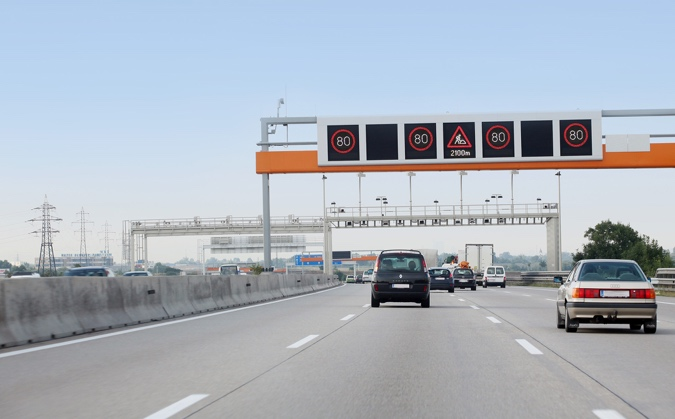
\includegraphics[width=0.9\linewidth]{image/dynamic_signage} \caption{Dynamic signage system in Austria (ASFiNAG, 2019b)}\label{fig:unnamed-chunk-5}
\end{figure}

With respect to the impact on the societal level, a Belgian study, by E. De Pauw et al.~showed a significant decrease (-18 \%) in the number of injury crashes after the introduction of a DSL system (De Pauw et al., 2018). F.G. Habtemichael and L. de Picado Santos (2013) found that a DSL system has the highest safety benefit during highly congested traffic conditions. The operational benefit in turn was the highest during lightly congested traffic conditions. However, the success of DSL is highly dependent on the level of driver compliance (Habtemichael \& de Picado Santos, 2013). Besides the safety aspects, the goal of DSL is to harmonize the traffic flow. Heavy traffic can cause shock waves, which result in longer travel times and large variations in the speeds of the vehicles. The latter again may lead to unsafe situations. By using DSL this phenomenon could be reduced (Hegyi et al., 2005). Traffic flow efficiency can be improved more, when DSL is combined with coordinated ramp metering (Carlson, 2010). Speed limits can also be temporary lowered, due to high emission values. If the emission values combined with the amount of traffic, reach a specific level, the DSL-System responds automatically and lowers the speed limit for a certain time. How high that level is, depends on the local policies (ASFiNAG, 2019c).

\hypertarget{key-stakeholders-4}{%
\subsection*{Key stakeholders}\label{key-stakeholders-4}}
\addcontentsline{toc}{subsection}{Key stakeholders}

\begin{itemize}
\tightlist
\item
  \textbf{Affected}: Motorways users
\item
  \textbf{Responsible}: Motorway Infrastructure Agencies, Technology Providers, Policymakers, State authorities
\end{itemize}

\hypertarget{current-state-of-art-in-research-4}{%
\subsection*{Current state of art in research}\label{current-state-of-art-in-research-4}}
\addcontentsline{toc}{subsection}{Current state of art in research}

Studies show, that in retrospect most DSL implementations in Europe were efficient traffic safety and flow improvement. In the United States the increase in safety was significant as well, but the flow improvement was controversial (Lu \& Shladover, 2014). Hassan et al.~(2012) discovered that during bad weather conditions the combination of Changeable Message Signs (CMS) and DSL was the best way to improve safety. Current research shows that the benefits of DSL systems could be improved by integrating it in a fully connected vehicles (CV) environment (Wu et al., 2020). Currently, research focuses on the integration of C-ITS, to connect the infrastructure to the vehicles. European standards should be developed during the next years (Erhart, 2019).

\hypertarget{current-state-of-art-in-practice-4}{%
\subsection*{Current state of art in practice}\label{current-state-of-art-in-practice-4}}
\addcontentsline{toc}{subsection}{Current state of art in practice}

DSL systems are implemented and used around the world. The used algorithms differ, however. DSL integrated with C-ITS has been implemented in a test environment (Erhart, 2019).
Austrian motorways are managed by the ASFiNAG - currently they have 17 DSL systems in use. That means that about 19 \% of the Austrian Motorway-System are currently equipped by an DSL system (ASFiNAG, 2019a). So, there is potential for expansion. One global player in traffic management is the Austrian company Kapsch TrafficCom. Worldwide they have implemented their systems on more than 3.500 km of motorway (Kapsch TrefficCom). Kapsch TrafficCom's approximately 5,000 employees generated revenues of EUR 738 million in the fiscal year 2018/19.

\hypertarget{relevant-initiatives-in-austria-4}{%
\subsection*{Relevant initiatives in Austria}\label{relevant-initiatives-in-austria-4}}
\addcontentsline{toc}{subsection}{Relevant initiatives in Austria}

\begin{itemize}
\tightlist
\item
  \href{https://www.asfinag.at/verkehrssicherheit/verkehrsmanagement/verkehrssteuerung/}{Asfinag}
\item
  \href{https://blog.asfinag.at/technik-innovation/c-its-vernetzte-autos-intelligenter-verkehr/}{Asifinag blog}
\item
  \href{https://www.kapsch.net/ktc/Portfolio/IMS/Congestion/Highway-Traffic-Management}{kapsch.net}
\item
  \href{https://www.strabag-iss.com/databases/internet/_public/content30.nsf/web30?Openagent\&id=DE-STRABAGISS-DE_verkehrstechnik.html\&men1=3\&men2=5\&sid=351}{strabag-iss.com}
\item
  \href{https://www.pke.at/index.php?id=17\#c117}{pke.at}
\item
  \href{http://www.aigner-stahlbau.at/leistungen/verkehrstechnik/}{aigner-stahlbau.at}
\end{itemize}

\hypertarget{impacts-with-respect-to-sustainable-development-goals-sdgs-4}{%
\subsection*{Impacts with respect to Sustainable Development Goals (SDGs)}\label{impacts-with-respect-to-sustainable-development-goals-sdgs-4}}
\addcontentsline{toc}{subsection}{Impacts with respect to Sustainable Development Goals (SDGs)}

\begin{longtable}[]{@{}ccccc@{}}
\toprule
\begin{minipage}[b]{0.17\columnwidth}\centering
Impact level\strut
\end{minipage} & \begin{minipage}[b]{0.16\columnwidth}\centering
Indicator\strut
\end{minipage} & \begin{minipage}[b]{0.17\columnwidth}\centering
Impact direction\strut
\end{minipage} & \begin{minipage}[b]{0.17\columnwidth}\centering
Goal description and number\strut
\end{minipage} & \begin{minipage}[b]{0.17\columnwidth}\centering
Source\strut
\end{minipage}\tabularnewline
\midrule
\endhead
\begin{minipage}[t]{0.17\columnwidth}\centering
Individual\strut
\end{minipage} & \begin{minipage}[t]{0.16\columnwidth}\centering
Fatal collisions reduced\strut
\end{minipage} & \begin{minipage}[t]{0.17\columnwidth}\centering
\textbf{+}\strut
\end{minipage} & \begin{minipage}[t]{0.17\columnwidth}\centering
Health \& Wellbeing (\emph{3})\strut
\end{minipage} & \begin{minipage}[t]{0.17\columnwidth}\centering
Hegyi et al., 2005\strut
\end{minipage}\tabularnewline
\begin{minipage}[t]{0.17\columnwidth}\centering
Individual\strut
\end{minipage} & \begin{minipage}[t]{0.16\columnwidth}\centering
Travel time reduced\strut
\end{minipage} & \begin{minipage}[t]{0.17\columnwidth}\centering
\textbf{+}\strut
\end{minipage} & \begin{minipage}[t]{0.17\columnwidth}\centering
Environmental sustainability (\emph{7,12,13,15})\strut
\end{minipage} & \begin{minipage}[t]{0.17\columnwidth}\centering
Habtemichael \& de Picado Santos, 2013\strut
\end{minipage}\tabularnewline
\begin{minipage}[t]{0.17\columnwidth}\centering
Systemic\strut
\end{minipage} & \begin{minipage}[t]{0.16\columnwidth}\centering
Fatal collisions reduced\strut
\end{minipage} & \begin{minipage}[t]{0.17\columnwidth}\centering
\textbf{+}\strut
\end{minipage} & \begin{minipage}[t]{0.17\columnwidth}\centering
Health \& Wellbeing (\emph{3})\strut
\end{minipage} & \begin{minipage}[t]{0.17\columnwidth}\centering
Hegyi et al., 2005\strut
\end{minipage}\tabularnewline
\begin{minipage}[t]{0.17\columnwidth}\centering
Systemic\strut
\end{minipage} & \begin{minipage}[t]{0.16\columnwidth}\centering
Annual greenhouse gas emissions decrease\strut
\end{minipage} & \begin{minipage}[t]{0.17\columnwidth}\centering
\textbf{+}\strut
\end{minipage} & \begin{minipage}[t]{0.17\columnwidth}\centering
Environmental sustainability (\emph{7,12-13,15})\strut
\end{minipage} & \begin{minipage}[t]{0.17\columnwidth}\centering
Schimany, 2011\strut
\end{minipage}\tabularnewline
\bottomrule
\end{longtable}

\hypertarget{technology-and-societal-readiness-level-4}{%
\subsection*{Technology and societal readiness level}\label{technology-and-societal-readiness-level-4}}
\addcontentsline{toc}{subsection}{Technology and societal readiness level}

\begin{longtable}[]{@{}cc@{}}
\toprule
TRL & SRL\tabularnewline
\midrule
\endhead
7-9 & 8-9\tabularnewline
\bottomrule
\end{longtable}

\hypertarget{open-questions-4}{%
\subsection*{Open questions}\label{open-questions-4}}
\addcontentsline{toc}{subsection}{Open questions}

\begin{enumerate}
\def\labelenumi{\arabic{enumi}.}
\tightlist
\item
  Which algorithms for DSL are the most efficient ones?
\item
  How can DSL be further developed?
\item
  How can fail-safe operation be improved?
\item
  How can DSL be combined with C-ITS?
\end{enumerate}

\hypertarget{references-4}{%
\subsection*{References}\label{references-4}}
\addcontentsline{toc}{subsection}{References}

\begin{itemize}
\tightlist
\item
  ASFiNAG. (2019a). Handlungsfelder. Retrieved 17th December 2020, from \url{http://verkehrssicherheit.asfinag.at/aktionsprogramme/handlungsfelder/}
\item
  ASFiNAG. (2019b). Verkehrsbeeinflussungsanlagen -- Für mehr Sicherheit: Arten von Verkehrsbeeinflussungsanlagen. Retrieved 11th December 2020, from \url{https://asfinag.azureedge.net/media/1607/vba-fotomontage.jpg}
\item
  ASFiNAG. (2019c). Verkehrsbeeinflussungsanlagen -- Für mehr Sicherheit: Die VBA und der ``Lufthunderter''. Retrieved 3rd December 2020, from \url{https://www.asfinag.at/verkehrssicherheit/verkehrsmanagement/verkehrssteuerung/}
\item
  Carlson, R. C., Papamichail, I., Papageorgiou, M., \& Messmer, A. (2010). Optimal motorway traffic flow control involving variable speed limits and ramp metering. Transportation Science, 44(2), 238-253.
\item
  De Pauw, E., Daniels, S., Franckx, L., \& Mayeres, I. (2018). Safety effects of dynamic speed limits on motorways. Accident Analysis \& Prevention, 114, 83-89.
\item
  Erhart, Jaqueline. (2019). Vernetzte Autos, intelligenter Verkehr: Was C-ITS ist, was es kann und wem es nutzt. Retrieved 17th December 2020, from \url{https://blog.asfinag.at/technik-innovation/c-its-vernetzte-autos-intelligenter-verkehr/}\\
\item
  Habtemichael, F. G., \& de Picado Santos, L. (2013). Safety and Operational Benefits of Variable Speed Limits under Different Traffic Conditions and Driver Compliance Levels. Transportation Research Record, 2386(1), 7--15. \url{https://doi.org/10.3141/2386-02}
\item
  Hassan, H. M., Abdel-Aty, M. A., Choi, K., \& Algadhi, S. A. (2012). Driver behavior and preferences for changeable message signs and variable speed limits in reduced visibility conditions. Journal of Intelligent Transportation Systems, 16(3), 132-146.
\item
  Hegyi, A., De Schutter, B., \& Hellendoorn, J. (2005). Optimal coordination of variable speed limits to suppress shock waves. IEEE Transactions on intelligent transportation systems, 6(1), 102-112.
\item
  Kapsch TrefficCom. Verkehrsmanagement auf Autobahnen. Retrieved 8th January 2021, \url{https://www.kapsch.net/ktc/Portfolio/IMS/Congestion/Highway-Traffic-Management}
\item
  Lu, X.-Y., \& Shladover, S. E. (2014). Review of Variable Speed Limits and Advisories: Theory, Algorithms, and Practice. Transportation Research Record, 2423(1), 15--23. \url{https://doi.org/10.3141/2423-03}
\item
  Mobility and Transport \textbar{} European Commission. (2020). Dynamic speed limits. Retrieved 2nd December 2020, from \url{https://ec.europa.eu/transport/road_safety/specialist/knowledge/speed/new_technologies_new_opportunities/dynamic_speed_limits_en}
\item
  Schimany, H. K. (2011). Blue Globe Foresight.
\item
  Wu, Y., Abdel-Aty, M., Wang, L., \& Rahman, M. S. (2020). Combined connected vehicles and variable speed limit strategies to reduce rear-end crash risk under fog conditions. Journal of Intelligent Transportation Systems, 24(5), 494-513.
\end{itemize}

\hypertarget{passengers-and-goods-fleet-management}{%
\section{Passengers and goods fleet management}\label{passengers-and-goods-fleet-management}}

\hypertarget{urban-access-management}{%
\section{Urban access management}\label{urban-access-management}}

\hypertarget{synonyms-5}{%
\subsection*{Synonyms}\label{synonyms-5}}
\addcontentsline{toc}{subsection}{Synonyms}

\emph{Access Regulation Schemes (ARS), Urban Vehicle Access Regulations (UVARs), Low Emission Zones (LEZ), Access Restrictions, Traffic Restrictions, Limited Traffic Zones, Permit Schemes}

\hypertarget{definition-5}{%
\subsection*{Definition}\label{definition-5}}
\addcontentsline{toc}{subsection}{Definition}

Urban Access Management can be seen as regulations, restrictions or bans, for traffic entering cities. Factors like congestion, air pollution, traffic noise or damage to historic buildings are influencing the liveability of cities negatively. Therefore, many cities have been introducing Access Regulation Schemes (ARS) with the goal of less vehicles entering the particular city or area. Implementing a pedestrian zone, is the simplest type of ARS and can improve the attractiveness of tourist attractions or shopping streets significantly (Sadler Consultants Europe GmbH, n.d. c). ARS can be differentiated by vehicle type, vehicle weight, by type of trip (e.g.~delivery), by driver (e.g.~residents or access), or applies to all vehicles (Sadler Consultants Europe GmbH, n.d. c). Furthermore, ARS can be static or dynamic, depending, for example, on the time of the day or air pollution levels. A list below provides examples of current measures used in the urban areas:

\begin{itemize}
\tightlist
\item
  Low Emission Zones (LEZ)
\item
  Limited Access Zones
\item
  Urban Toll Schemes / Congestion Charging (CS)
\item
  Emergency Air Pollution Schemes
\item
  Zero Emission Zones (ZEZ)
\item
  Other Access Regulations (like Limited Traffic Zones, Through traffic bans, `Superblocks´ etc.)
\item
  Smaller Regulations / Restrictions (like school streets or shared spaces) (Sandler Consultants Europe GmbH, n.d. d).
\end{itemize}

Solutions for ARS can be enforced by physical barriers or cameras, based on automatic number plate recognition (ANPR) systems and/or dedicated short-range communication (DSRC) technology, using on-board units (OBUs) (Kapsch TrafficCom., n.d. b) or by police or local authority officers (Sadler Consultants Europe GmbH, n.d. c).

The impact of Urban Vehicle Access Regulations differs according the implemented schemes, but several common goals are addressed:
- Air quality improvement
- Traffic congestion reduction
- Urban landscape preservation (historical town centres)
- Climate change mitigation
- Quality of life
- Noise mitigation
- Road safety
- Raising revenues (Sandler Consultants Europe GmbH, n.d. d).

In Austria, several cities and regions have implemented Low Emission Zones (LEZ) for lorries. For example, the city of Salzburg has Access Regulations (AR) for the city centre in place, so only vehicles with a specific reason (delivery or police) are allowed to enter. On the other hand, Tirol introduces occasionally traffic bans during the summer months (Sandler Consultants Europe GmbH, n.d. a). While, the city of Vienna aims at implementing a traffic-calmed city centre by 2022 (Stadt Wien, 2020).

\hypertarget{key-stakeholders-5}{%
\subsection*{Key stakeholders}\label{key-stakeholders-5}}
\addcontentsline{toc}{subsection}{Key stakeholders}

\begin{itemize}
\tightlist
\item
  \textbf{Affected}: Car Users -- especially users of old or high polluting cars, truck drivers, Shippers/producers, Wholesalers, Logistics providers, Retailers, Consumers, Citizens, Authorities
\item
  \textbf{Responsible}: Municipalities, Road Operators, Urban Traffic Management, Authorities
\end{itemize}

\hypertarget{current-state-of-art-in-research-5}{%
\subsection*{Current state of art in research}\label{current-state-of-art-in-research-5}}
\addcontentsline{toc}{subsection}{Current state of art in research}

Current research addresses the evaluation of UVAR implementations and identifies their positive and negative effects. For example, Lopez (2018) found that Urban Consolidation Centres (UCCs), Cargo Bikes (CBs) and Off-hour Deliveries (OHDs) are the three preferred types of solutions to assist in mitigating unwanted side-effects of UVARs on the logistic sector. Further, current research focuses on the sustainable urban planning in cites affected by mass tourism (García Hernández, 2019; Nolasco‐Cirugeda, 2020). Additionally, most recent area of research deals with geofencing that aims at creating digital zones defined on a map, with specific rules, that can be transmitted to the vehicles (Arnesen et al., 2020).

\hypertarget{current-state-of-art-in-practice-5}{%
\subsection*{Current state of art in practice}\label{current-state-of-art-in-practice-5}}
\addcontentsline{toc}{subsection}{Current state of art in practice}

According to Lopez (2018) there are the two preferred UVAR schemes: Low Emission Zones (LEZ) and Congestion Charging (CC). The implementation of these schemes is widely spread within Europe but follows different approaches. Lopez (2018) identified two dominant LEZ enforcement models, first visual surveillance using windscreen stickers and second, cameras with ANPR technology. Furthermore it is argued that \emph{``It is very important to consider that the degree of impact of each measure not only varies from city to city but also depends on the presence of a mix of access regulations``} (Lopez, 2018).

\hypertarget{relevant-initiatives-in-austria-5}{%
\subsection*{Relevant initiatives in Austria}\label{relevant-initiatives-in-austria-5}}
\addcontentsline{toc}{subsection}{Relevant initiatives in Austria}

\begin{itemize}
\tightlist
\item
  \href{https://www.ris.bka.gv.at/GeltendeFassung.wxe?Abfrage=LrW\&Gesetzesnummer=20000270}{ris.bka.gv.at}
\item
  \href{https://www.wien.gv.at/ma22-lgb/luftgi.htm}{wien.gv.at}
\item
  \href{https://www.kapsch.net/ktc/its-solutions/urban-access-management/access-restriction/}{kapsch.net}
\end{itemize}

\hypertarget{impacts-with-respect-to-sustainable-development-goals-sdgs-5}{%
\subsection*{Impacts with respect to Sustainable Development Goals (SDGs)}\label{impacts-with-respect-to-sustainable-development-goals-sdgs-5}}
\addcontentsline{toc}{subsection}{Impacts with respect to Sustainable Development Goals (SDGs)}

\begin{longtable}[]{@{}ccccc@{}}
\toprule
\begin{minipage}[b]{0.17\columnwidth}\centering
Impact level\strut
\end{minipage} & \begin{minipage}[b]{0.16\columnwidth}\centering
Indicator\strut
\end{minipage} & \begin{minipage}[b]{0.17\columnwidth}\centering
Impact direction\strut
\end{minipage} & \begin{minipage}[b]{0.17\columnwidth}\centering
Goal description and number\strut
\end{minipage} & \begin{minipage}[b]{0.17\columnwidth}\centering
Source\strut
\end{minipage}\tabularnewline
\midrule
\endhead
\begin{minipage}[t]{0.17\columnwidth}\centering
Individual\strut
\end{minipage} & \begin{minipage}[t]{0.16\columnwidth}\centering
Noise \& pollution reduced\strut
\end{minipage} & \begin{minipage}[t]{0.17\columnwidth}\centering
\textbf{+}\strut
\end{minipage} & \begin{minipage}[t]{0.17\columnwidth}\centering
Health \& Wellbeing (\emph{3})\strut
\end{minipage} & \begin{minipage}[t]{0.17\columnwidth}\centering
Sandler Consultants Europe GmbH, n.d. b\strut
\end{minipage}\tabularnewline
\begin{minipage}[t]{0.17\columnwidth}\centering
Individual\strut
\end{minipage} & \begin{minipage}[t]{0.16\columnwidth}\centering
Travel time \& congestion reduced\strut
\end{minipage} & \begin{minipage}[t]{0.17\columnwidth}\centering
\textbf{+}\strut
\end{minipage} & \begin{minipage}[t]{0.17\columnwidth}\centering
Sustainable economic development (\emph{8,11})\strut
\end{minipage} & \begin{minipage}[t]{0.17\columnwidth}\centering
Sandler Consultants Europe GmbH, n.d. b\strut
\end{minipage}\tabularnewline
\begin{minipage}[t]{0.17\columnwidth}\centering
Systemic\strut
\end{minipage} & \begin{minipage}[t]{0.16\columnwidth}\centering
Road safety increased\strut
\end{minipage} & \begin{minipage}[t]{0.17\columnwidth}\centering
\textbf{+}\strut
\end{minipage} & \begin{minipage}[t]{0.17\columnwidth}\centering
Health \& Wellbeing (\emph{3})\strut
\end{minipage} & \begin{minipage}[t]{0.17\columnwidth}\centering
Sandler Consultants Europe GmbH, n.d. b\strut
\end{minipage}\tabularnewline
\begin{minipage}[t]{0.17\columnwidth}\centering
Systemic\strut
\end{minipage} & \begin{minipage}[t]{0.16\columnwidth}\centering
Space for sustainable transport users increased\strut
\end{minipage} & \begin{minipage}[t]{0.17\columnwidth}\centering
\textbf{+}\strut
\end{minipage} & \begin{minipage}[t]{0.17\columnwidth}\centering
Equality (\emph{5,10})\strut
\end{minipage} & \begin{minipage}[t]{0.17\columnwidth}\centering
Sandler Consultants Europe GmbH, n.d. d\strut
\end{minipage}\tabularnewline
\begin{minipage}[t]{0.17\columnwidth}\centering
Systemic\strut
\end{minipage} & \begin{minipage}[t]{0.16\columnwidth}\centering
Air quality improved\strut
\end{minipage} & \begin{minipage}[t]{0.17\columnwidth}\centering
\textbf{+}\strut
\end{minipage} & \begin{minipage}[t]{0.17\columnwidth}\centering
Environmental sustainability (\emph{7,12,13,15})\strut
\end{minipage} & \begin{minipage}[t]{0.17\columnwidth}\centering
Sandler Consultants Europe GmbH, n.d. d\strut
\end{minipage}\tabularnewline
\begin{minipage}[t]{0.17\columnwidth}\centering
Systemic\strut
\end{minipage} & \begin{minipage}[t]{0.16\columnwidth}\centering
Congestion reduced, revenues increased\strut
\end{minipage} & \begin{minipage}[t]{0.17\columnwidth}\centering
\textbf{+}\strut
\end{minipage} & \begin{minipage}[t]{0.17\columnwidth}\centering
Sustainable economic development (\emph{8,11})\strut
\end{minipage} & \begin{minipage}[t]{0.17\columnwidth}\centering
Sandler Consultants Europe GmbH, n.d. b\strut
\end{minipage}\tabularnewline
\begin{minipage}[t]{0.17\columnwidth}\centering
Systemic\strut
\end{minipage} & \begin{minipage}[t]{0.16\columnwidth}\centering
Urban landscape preservation\strut
\end{minipage} & \begin{minipage}[t]{0.17\columnwidth}\centering
\textbf{+}\strut
\end{minipage} & \begin{minipage}[t]{0.17\columnwidth}\centering
Innovation \& Infrastructure (\emph{9})\strut
\end{minipage} & \begin{minipage}[t]{0.17\columnwidth}\centering
Sandler Consultants Europe GmbH, n.d. b\strut
\end{minipage}\tabularnewline
\bottomrule
\end{longtable}

\hypertarget{technology-and-societal-readiness-level-5}{%
\subsection*{Technology and societal readiness level}\label{technology-and-societal-readiness-level-5}}
\addcontentsline{toc}{subsection}{Technology and societal readiness level}

\begin{longtable}[]{@{}cc@{}}
\toprule
TRL & SRL\tabularnewline
\midrule
\endhead
7-9 & 7-9\tabularnewline
\bottomrule
\end{longtable}

\hypertarget{open-questions-5}{%
\subsection*{Open questions}\label{open-questions-5}}
\addcontentsline{toc}{subsection}{Open questions}

\begin{enumerate}
\def\labelenumi{\arabic{enumi}.}
\tightlist
\item
  What effect will autonomous vehicles have on Urban Access Management?
\item
  How can geofencing be implemented on a wider scale and what are the barriers?
\item
  What standards would be useful to aggregate, to support affected stakeholders?
\item
  How can Urban Access Management engage with the Internet of Things (IoT)?
\end{enumerate}

\hypertarget{further-links-3}{%
\subsection*{Further links}\label{further-links-3}}
\addcontentsline{toc}{subsection}{Further links}

\begin{itemize}
\tightlist
\item
  \href{https://urbanaccessregulations.eu/urban-access-regulations/what-are-urban-access-regulations}{urbanaccessregulations.eu-1}
\item
  \href{https://urbanaccessregulations.eu/countries-mainmenu-147/austria-mainmenu-78/wien-vienna-emergency-scheme}{urbanaccessregulations.eu-2}
\end{itemize}

\hypertarget{references-5}{%
\subsection*{References}\label{references-5}}
\addcontentsline{toc}{subsection}{References}

\begin{itemize}
\tightlist
\item
  Arnesen, P., Seter, H., Foss, T., Dahl, E., Lillestøl, P. J., \& Jenssen, G. (2020). Geofencing for smart urban mobility. Summarizing the main findings of work package 2: Pilot Design and work package 3: Piloting.
\item
  García Hernández, M., Ivars-Baidal, J., \& Mendoza de Miguel, S. (2019). Overtourism in urban destinations: the myth of smart solutions.
\item
  Kapsch TrafficCom. (n.d. a). Access management \textbar{} Kapsch. Retrieved January 27, 2021, from \url{https://www.kapsch.net/ktc/Portfolio/IMS/Smart-Urban-Mobility/Access-Management}
\item
  Kapsch TrafficCom. (n.d. b). Limited Access Zone \textbar{} Kapsch. Retrieved January 27, 2021, from \url{https://www.kapsch.net/ktc/its-solutions/urban-access-management/access-restriction/}
\item
  Lopez, O. N. (2018). Urban vehicle access regulations. In Sustainable Freight Transport (pp.~139-163). Springer, Cham.
\item
  Nolasco‐Cirugeda, A., Martí, P., \& Ponce, G. (2020). Keeping mass tourism destinations sustainable via urban design: The case of Benidorm. Sustainable Development, 28(5), 1289-1303.
\item
  Sandler Consultants Europe GmbH. (n.d. a). Austria. Retrieved February 1, 2021, from \url{https://urbanaccessregulations.eu/countries-mainmenu-147/austria-mainmenu-78}
\item
  Sandler Consultants Europe GmbH. (n.d. b). Overview of website. Retrieved February 1, 2021, from \url{https://urbanaccessregulations.eu/userhome/general-overview\#Why\%20Access\%20\%20Regulations}\\
\item
  Sadler Consultants Europe GmbH. (n.d. c). Urban Access Regulations in Europe. Retrieved 26th January 2021, from \url{https://urbanaccessregulations.eu/about-us}
\item
  Sandler Consultants Europe GmbH. (n.d. d). What are Access Regulations? Retrieved February 1, 2021, from \url{https://urbanaccessregulations.eu/userhome/what-are-access-regulations-uvars-or-urban-vehicle-access-regulations}
\item
  Stadt Wien. (2020). Smarte Mobilität - Die Fortschrittskoalition für Wien. Retrieved February 1, 2021, from \url{https://www.wien.gv.at/regierungsabkommen2020/smart-city-wien/smarte-mobilitat/}
\end{itemize}

\hypertarget{digital}{%
\chapter{Digital road infrastructure and connectivity}\label{digital}}

\hypertarget{vehicle-to-infrastructure-communication}{%
\section{Vehicle to infrastructure communication}\label{vehicle-to-infrastructure-communication}}

\hypertarget{infrastructure-support-levels-for-automated-driving}{%
\section{Infrastructure support levels for automated driving}\label{infrastructure-support-levels-for-automated-driving}}

\hypertarget{vehicle-to-vehicle-communication}{%
\section{Vehicle to vehicle communication}\label{vehicle-to-vehicle-communication}}

\hypertarget{wireless-communication}{%
\section{Wireless communication}\label{wireless-communication}}

\hypertarget{passenger}{%
\chapter{Passenger information system}\label{passenger}}

\hypertarget{digital-journey-planner}{%
\section{Digital journey planner}\label{digital-journey-planner}}

\hypertarget{rail-telematics-for-passenger-services}{%
\section{Rail telematics for passenger services}\label{rail-telematics-for-passenger-services}}

\hypertarget{multimodal-information-and-route-planning}{%
\section{Multimodal information and route planning}\label{multimodal-information-and-route-planning}}

\hypertarget{real-time-location-based-information}{%
\section{Real-time, location-based information}\label{real-time-location-based-information}}

\hypertarget{multimodal}{%
\chapter{Multimodal integrated system}\label{multimodal}}

\hypertarget{first-last-mile-solutions}{%
\section{First-last mile solutions}\label{first-last-mile-solutions}}

\hypertarget{distance-or-time-based-fares}{%
\section{Distance or time-based fares}\label{distance-or-time-based-fares}}

\hypertarget{mobility-as-a-service}{%
\section{Mobility as a service}\label{mobility-as-a-service}}

\hypertarget{park-and-ride}{%
\section{Park and ride}\label{park-and-ride}}

\hypertarget{contactless-public-transport-cards}{%
\section{Contactless public transport cards}\label{contactless-public-transport-cards}}

\hypertarget{synonyms-6}{%
\subsection*{Synonyms}\label{synonyms-6}}
\addcontentsline{toc}{subsection}{Synonyms}

\emph{Contactless smart card, smart card ticketing}

\hypertarget{definition-6}{%
\subsection*{Definition}\label{definition-6}}
\addcontentsline{toc}{subsection}{Definition}

Smart card ticketing means, that the passenger's entitlement to travel is stored electronically on a chip that is usually embedded in a plastic card and validated when the card is presented to a smart reader (Turner \& Wilson, 2010). On the contrary to contact smart cards, which have to be inserted into a smart card reader, contactless smart cards must only be near to the readers (about 10 cm) to exchange data (Mezghani, 2008). There are three types of standards used, called Type A, Type B (both complying with ISO 14443 standard) and FeliCa, while FeliCa provides faster transmission and is mainly used in Asian countries (Kurauchi \& Schmöcker, 2017).
Smart and integrated ticketing systems are expected to deliver greater flexibility and simplicity for passengers, by offering increased speed, convenience and security against loss and theft (Turner \& Wilson, 2010). Economic and societal benefits from smart cards ticketing include the reduction in costs as a result of fewer paper tickets being sold, reduced queuing time, faster throughput of passengers at ticket gates, reduced boarding time for buses and reduced loss of revenue through fraud (Turner \& Wilson, 2010).
England's Department of Transport has planned a strategy, to introduce integrated and smart ticketing to the majority of the UK by 2020. Their research suggests that net annual benefits of over £1 billion per year to passengers, operators and local authorities can be the result (Turner \& Wilson, 2010).
Another advantage of using smart cards ticketing, is the large amount of data on passengers' behaviour, which can be collected with lower cost (Kurauchi \& Schmöcker, 2017). In Austria smart cards have not been implemented on a large scale. Only the City of Wales has smart cards for the public transport in use (Wels Linien). ÖBB (ÖBB, 2021) and Wiener Linien (Wiener Linien, 2021) don't have smart cards in use, but online tickets for smart phones, using QR Codes. Wiener Linien are currently researching on a more efficient solution for the usage of digital tickets, since they developed, that ticket controls of digital tickets take longer than for paper tickets (Wiener Linien, 2021b).

\hypertarget{key-stakeholders-6}{%
\subsection*{Key stakeholders}\label{key-stakeholders-6}}
\addcontentsline{toc}{subsection}{Key stakeholders}

\begin{itemize}
\tightlist
\item
  \textbf{Affected}: Public transport users, ticket inspectors
\item
  \textbf{Responsible}: Public transport operators, public transport associations, public transport authorities, smart card producers, Industry suppliers
\end{itemize}

\hypertarget{current-state-of-art-in-research-6}{%
\subsection*{Current state of art in research}\label{current-state-of-art-in-research-6}}
\addcontentsline{toc}{subsection}{Current state of art in research}

The latest research goes in the direction of using smart phones or other mobile devices for smart ticketing. An initiative, led by NFC Forum and GSMA achieved in 2015 together with global public transport representatives, the Smart Ticketing Alliance and the JR East as well as standards bodies, including CEN and ISO, harmonizing the specifications of mobile device NFC interfaces and public transport readers and cards. Together they established standards for testing mobile devices and public transport equipment (NFC Forum, 2016).

\begin{figure}
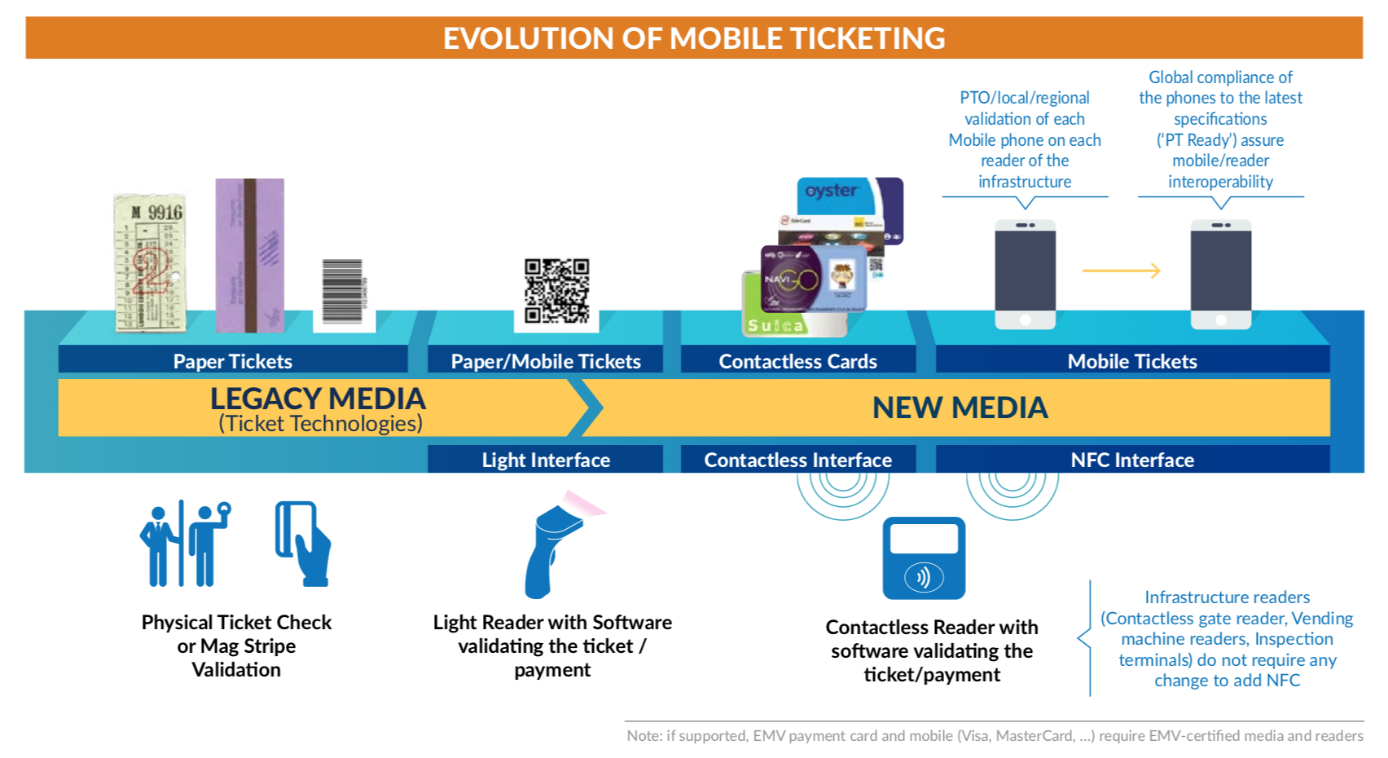
\includegraphics[width=0.9\linewidth]{image/smart_cards} \caption{The evolution of mobile ticketing (NFC Forum, 2016)}\label{fig:unnamed-chunk-6}
\end{figure}

Furthermore current research addresses the issues of big data and how collected data through contactless smart cards can be best analysed (see Kurauchi \& Schmöcker, 2017).

\hypertarget{current-state-of-art-in-practice-6}{%
\subsection*{Current state of art in practice}\label{current-state-of-art-in-practice-6}}
\addcontentsline{toc}{subsection}{Current state of art in practice}

Many countries, regions or cities, have smart card ticketing systems in use, like the whole of Netherlands, Helsinki Region, Minsk, Berlin, Auckland, Sydney and many more (see Wikipedia contributors, 2021). The systems itself differ and depend on the local ticketing and fare systems. While London, for instance, is using an access control system, Helsinki's system is trust based. Furthermore, a distinction can be made between pre-paid (debit) and post-paid (credit) systems (Kurauchi \& Schmöcker, 2017).

\hypertarget{relevant-initiatives-in-austria-6}{%
\subsection*{Relevant initiatives in Austria}\label{relevant-initiatives-in-austria-6}}
\addcontentsline{toc}{subsection}{Relevant initiatives in Austria}

\begin{itemize}
\tightlist
\item
  \href{https://taikai.network/en/wiener-linien/challenges/tickethon}{taikai.network}
\item
  \href{https://www.variuscard.com/}{variuscard}
\item
  \href{https://www.austriacard.com/}{austriacard}
\end{itemize}

\hypertarget{impacts-with-respect-to-sustainable-development-goals-sdgs-6}{%
\subsection*{Impacts with respect to Sustainable Development Goals (SDGs)}\label{impacts-with-respect-to-sustainable-development-goals-sdgs-6}}
\addcontentsline{toc}{subsection}{Impacts with respect to Sustainable Development Goals (SDGs)}

\begin{longtable}[]{@{}ccccc@{}}
\toprule
\begin{minipage}[b]{0.17\columnwidth}\centering
Impact level\strut
\end{minipage} & \begin{minipage}[b]{0.16\columnwidth}\centering
Indicator\strut
\end{minipage} & \begin{minipage}[b]{0.17\columnwidth}\centering
Impact direction\strut
\end{minipage} & \begin{minipage}[b]{0.17\columnwidth}\centering
Goal description and number\strut
\end{minipage} & \begin{minipage}[b]{0.17\columnwidth}\centering
Source\strut
\end{minipage}\tabularnewline
\midrule
\endhead
\begin{minipage}[t]{0.17\columnwidth}\centering
Individual\strut
\end{minipage} & \begin{minipage}[t]{0.16\columnwidth}\centering
Personal, travel expenditure reduced\strut
\end{minipage} & \begin{minipage}[t]{0.17\columnwidth}\centering
\textbf{+}\strut
\end{minipage} & \begin{minipage}[t]{0.17\columnwidth}\centering
Sustainable economic development (\emph{8,11})\strut
\end{minipage} & \begin{minipage}[t]{0.17\columnwidth}\centering
Turner \& Wilson, 2010\strut
\end{minipage}\tabularnewline
\begin{minipage}[t]{0.17\columnwidth}\centering
Individual\strut
\end{minipage} & \begin{minipage}[t]{0.16\columnwidth}\centering
Access to digitalised transport\strut
\end{minipage} & \begin{minipage}[t]{0.17\columnwidth}\centering
\textbf{+}\strut
\end{minipage} & \begin{minipage}[t]{0.17\columnwidth}\centering
Innovation \& Infrastructure (\emph{9})\strut
\end{minipage} & \begin{minipage}[t]{0.17\columnwidth}\centering
Turner \& Wilson, 2010\strut
\end{minipage}\tabularnewline
\begin{minipage}[t]{0.17\columnwidth}\centering
Systemic\strut
\end{minipage} & \begin{minipage}[t]{0.16\columnwidth}\centering
Public transport capacity increases\strut
\end{minipage} & \begin{minipage}[t]{0.17\columnwidth}\centering
\textbf{+}\strut
\end{minipage} & \begin{minipage}[t]{0.17\columnwidth}\centering
Sustainable economic development (\emph{8,11})\strut
\end{minipage} & \begin{minipage}[t]{0.17\columnwidth}\centering
Turner \& Wilson, 2010\strut
\end{minipage}\tabularnewline
\begin{minipage}[t]{0.17\columnwidth}\centering
Systemic\strut
\end{minipage} & \begin{minipage}[t]{0.16\columnwidth}\centering
Facilitates integration of the fare systems of several operators within a city\strut
\end{minipage} & \begin{minipage}[t]{0.17\columnwidth}\centering
\textbf{+}\strut
\end{minipage} & \begin{minipage}[t]{0.17\columnwidth}\centering
Partnership \& collaborations (\emph{17})\strut
\end{minipage} & \begin{minipage}[t]{0.17\columnwidth}\centering
Kurauchi \& Schmoecker, 2017\strut
\end{minipage}\tabularnewline
\bottomrule
\end{longtable}

\hypertarget{technology-and-societal-readiness-level-6}{%
\subsection*{Technology and societal readiness level}\label{technology-and-societal-readiness-level-6}}
\addcontentsline{toc}{subsection}{Technology and societal readiness level}

\begin{longtable}[]{@{}cc@{}}
\toprule
TRL & SRL\tabularnewline
\midrule
\endhead
7-9 & 7-9\tabularnewline
\bottomrule
\end{longtable}

\hypertarget{open-questions-6}{%
\subsection*{Open questions}\label{open-questions-6}}
\addcontentsline{toc}{subsection}{Open questions}

\begin{enumerate}
\def\labelenumi{\arabic{enumi}.}
\tightlist
\item
  How can the large amount of provided data be best used?
\item
  What advantages and disadvantages would an implementation in the main cities of Austria have?
\end{enumerate}

\hypertarget{further-links-4}{%
\subsection*{Further links}\label{further-links-4}}
\addcontentsline{toc}{subsection}{Further links}

\begin{itemize}
\tightlist
\item
  \href{https://www.itso.org.uk/}{itso}
\end{itemize}

\hypertarget{references-6}{%
\subsection*{References}\label{references-6}}
\addcontentsline{toc}{subsection}{References}

\begin{itemize}
\tightlist
\item
  Kurauchi, F., \& Schmöcker, J. D. (Eds.). (2017). Public transport planning with smart card data. CRC Press.
\item
  Mezghani, M. (2008). Study on electronic ticketing in public transport. European Metropolitan Transport Authorities (EMTA), 56, 38.
\item
  NFC Forum. (2016). NFC-enabled e-Ticketing in Public Transport\,: Clearing the Route to Interoperability. December. \url{https://nfc-forum.org/wp-content/uploads/2016/12/NFC_enabled_eTicketing_in_Public_Transport_White_Paper.pdf}
\item
  ÖBB. Ihr Weg zum Ticket. Retrieved 13th January 2021, from \url{https://www.oebb.at/de/tickets-kundenkarten/weg-zum-ticket}
\item
  Turner, M., \& Wilson, R. (2010). Smart and integrated ticketing in the UK: Piecing together the jigsaw. Computer Law \& Security Review, 26(2), 170-177.
\item
  Wels Linien. Tarife. Retrieved 13th January 2021, from \url{https://www.welslinien.at/tarife/}
\item
  Wiener Linien. (2021a). Der richtige Fahrschein,
  der passende Tarif. Retrieved 13th January 2021, from \url{https://www.wienerlinien.at/eportal3/ep/channelView.do/pageTypeId/66526/channelId/-46648}
\item
  Wiener Linien. (2021b). Digital-Wettbewerb ``Vienna Tickethon'' gestartet. Retrieved 13th January 2021, from \url{https://www.wienerlinien.at/eportal3/ep/contentView.do/pageTypeId/66526/programId/74577/contentTypeId/1001/channelId/-47186/contentId/5002360\#}:\textasciitilde:text=Im\%20Rahmen\%20eines\%20internationalen\%20Hackathon,Wettbewerb\%20l\%C3\%A4uft\%20bis\%20Anfang\%20M\%C3\%A4rz
\item
  Wikipedia contributors. (2021, January 8). List of smart cards. In Wikipedia, The Free Encyclopedia. Retrieved 15:30, January 13, 2021, from \url{https://en.wikipedia.org/w/index.php?title=List_of_smart_cards\&oldid=999040130}
\end{itemize}

\hypertarget{information-and-assistance-for-people-with-special-needs}{%
\section{Information and assistance for people with special needs}\label{information-and-assistance-for-people-with-special-needs}}

\hypertarget{mobilityfreight-hubs}{%
\section{Mobility/Freight hubs}\label{mobilityfreight-hubs}}

\hypertarget{connected}{%
\chapter{Connected and autonomous driving}\label{connected}}

\hypertarget{parking-infrastructure-for-autonomous-vehicles}{%
\section{Parking infrastructure for autonomous vehicles}\label{parking-infrastructure-for-autonomous-vehicles}}

\hypertarget{connected-vehicles}{%
\section{Connected vehicles}\label{connected-vehicles}}

\hypertarget{automated-vehicles}{%
\section{Automated vehicles}\label{automated-vehicles}}

\hypertarget{onboard}{%
\chapter{On-board technology for connected and automated vehicles}\label{onboard}}

\hypertarget{advanced-driver-assistance-system}{%
\section{Advanced driver assistance system}\label{advanced-driver-assistance-system}}

\hypertarget{parking-assistance-system}{%
\section{Parking assistance system}\label{parking-assistance-system}}

\hypertarget{lane-keeping}{%
\section{Lane keeping}\label{lane-keeping}}

\hypertarget{distane-keeping}{%
\section{Distane keeping}\label{distane-keeping}}

\hypertarget{crash-avoidance}{%
\section{Crash avoidance}\label{crash-avoidance}}

\hypertarget{mainteinance-assistance}{%
\section{Mainteinance assistance}\label{mainteinance-assistance}}

\hypertarget{digital-maps}{%
\section{Digital maps}\label{digital-maps}}

\hypertarget{e-horizon}{%
\section{E-Horizon}\label{e-horizon}}

\hypertarget{emergency-call}{%
\section{Emergency call}\label{emergency-call}}

\hypertarget{freight}{%
\chapter{Freight and commercial transport}\label{freight}}

\hypertarget{automated-road-freight}{%
\section{Automated road freight}\label{automated-road-freight}}

\hypertarget{freight-dreyage-optimisation}{%
\section{Freight dreyage optimisation}\label{freight-dreyage-optimisation}}

\hypertarget{tracking-and-tracing-of-dangerous-goods}{%
\section{Tracking and tracing of dangerous goods}\label{tracking-and-tracing-of-dangerous-goods}}

\hypertarget{intermodal-freight}{%
\section{Intermodal Freight}\label{intermodal-freight}}

\hypertarget{real-time-disruption-management-and-route-planning}{%
\section{Real-time disruption management and route planning}\label{real-time-disruption-management-and-route-planning}}

\hypertarget{traffic-signal-control}{%
\section{Traffic signal control}\label{traffic-signal-control}}

\hypertarget{urban-deliveries}{%
\section{Urban Deliveries}\label{urban-deliveries}}

\hypertarget{parcel-load-pooling}{%
\section{Parcel load pooling}\label{parcel-load-pooling}}

\hypertarget{intelligent-truck-parking-and-delivery-space-booking}{%
\section{Intelligent truck parking and delivery space booking}\label{intelligent-truck-parking-and-delivery-space-booking}}

\hypertarget{delivery-drones}{%
\section{Delivery drones}\label{delivery-drones}}

\hypertarget{commercial-vehicle-on-board-safety-systems}{%
\section{Commercial vehicle on-board safety systems}\label{commercial-vehicle-on-board-safety-systems}}

\hypertarget{truck-platooning}{%
\section{Truck Platooning}\label{truck-platooning}}

\hypertarget{rail-telematics-for-freight-services}{%
\section{Rail telematics for freight services}\label{rail-telematics-for-freight-services}}

\hypertarget{electric-vehicle-delivery-fleets}{%
\section{Electric vehicle delivery fleets}\label{electric-vehicle-delivery-fleets}}

\hypertarget{multimodal-transport-management-systems}{%
\section{Multimodal transport management systems}\label{multimodal-transport-management-systems}}

\hypertarget{cooperative-adaptive-cruise-control-in-trucks}{%
\section{Cooperative adaptive cruise control in trucks}\label{cooperative-adaptive-cruise-control-in-trucks}}

\hypertarget{collective}{%
\chapter{Collective mobility vehicles}\label{collective}}

\hypertarget{demand-responsive-transit}{%
\section{Demand responsive transit}\label{demand-responsive-transit}}

\hypertarget{personal-rapid-transit}{%
\section{Personal rapid transit}\label{personal-rapid-transit}}

\hypertarget{bus-rapid-transit}{%
\section{Bus rapid transit}\label{bus-rapid-transit}}

\hypertarget{light-rail-transit}{%
\section{Light rail transit}\label{light-rail-transit}}

\hypertarget{passenger-drones}{%
\section{Passenger drones}\label{passenger-drones}}

\hypertarget{synonyms-7}{%
\subsection*{Synonyms}\label{synonyms-7}}
\addcontentsline{toc}{subsection}{Synonyms}

\emph{urban air mobility (UAM), vertical take-off and landing (VTOL), unmanned aerial vehicles (UAVs)}

\hypertarget{definition-7}{%
\subsection*{Definition}\label{definition-7}}
\addcontentsline{toc}{subsection}{Definition}

Drones or unmanned aerial vehicles (UAVs) could become the most iconic technology of the 21st century. Drones combine three key principles of technological modernity - computing, autonomy and limitless mobility. Capabilities that until now could only be used by the military are becoming accessible to most of the population. Potential use cases for drones range from surveillance and reconnaissance missions to novel forms of logistics and personal transport. The commercial use of drones is associated with enormous economic opportunities. However, even though drones are already common as surveillance/sensing devices in security services, geodesy or agriculture, their use as a means of transport is still at the beginning (Kellermann et al., 2020).
Delivery drones are currently able to lift weights of up to 2-3 kg and carry out flight missions in an urban space (Kellermann et al., 2020). However, passenger drones have also already demonstrated the technical ability to transport passengers within or between cities (LeBeau, 2016; Holt, 2018; Hawkins, 2018). It is not only a historic turning point in aviation, but the beginning of a new era in which flat airspace could become the ``third dimension'' of transport (Kellermann et al., 2020).
The name of the new type of vehicle is still far from being agreed internationally. There are several names to choose from, such as passenger drone, manned multicopter, Passenger Air Vehicle (PAV), Electric Vertical Take-off and Landing Aircraft (EVTOL), autonomous air taxis, unmanned aerial taxis, flying cars or even a new term (Pramer \& Sommavilla, 2020).
The autonomous air taxis will be a mixture of helicopter and drone. But this also means that they will be vertical take-off and landing (VTOL) vehicles.
There are several reasons why drone-related industries are being supported significantly. One of the reasons is that the airspace is still fairly free of traffic. The risk of collisions is (relatively) low and autopilots for aircraft have long been established. Industry experts therefore suspect that we could see self-flying air taxis even before self-driving cars. Being able to do without pilots would make an air taxi service even cheaper and make it possible for more people to afford it (UNIQA, 2019).
The European Commission estimates the economic impact at €10 billion annually until 2035 and foresees the creation of more than 100,000 direct jobs. Taking into account indirect macroeconomic effects in drone-related industries, the Commission even projects 250,000 to 400,000 additional jobs (SESAR, 2016).

\hypertarget{key-stakeholders-7}{%
\subsection*{Key stakeholders}\label{key-stakeholders-7}}
\addcontentsline{toc}{subsection}{Key stakeholders}

\begin{itemize}
\tightlist
\item
  \textbf{Affected}: Citizen, Insurers
\item
  \textbf{Responsible}: National Governments, City government, Private Companies
\end{itemize}

\hypertarget{current-state-of-art-in-research-7}{%
\subsection*{Current state of art in research}\label{current-state-of-art-in-research-7}}
\addcontentsline{toc}{subsection}{Current state of art in research}

Since all prototypes are owned by private companies and the technology is not really shared due to competition, there are few technical research papers.
The media analysis about drones for parcel and passenger transportation shows that currently the research is focused in the following areas (see table below):

\begin{longtable}[]{@{}ccc@{}}
\toprule
Topics & Percentage & Number of studies\tabularnewline
\midrule
\endhead
General Surveys & 18.9\% & 21\tabularnewline
Logistics (general) & 18.0\% & 20\tabularnewline
Attitude and Acceptance Research & 13.5\% & 15\tabularnewline
Law and Regulations & 11.7\% & 13\tabularnewline
Ethics and Technology Assessment & 10.8\% & 12\tabularnewline
Sustainability Assessment & 8.1\% & 9\tabularnewline
Urban and Transportation Planning & 7.2\% & 8\tabularnewline
Political agenda/strategies & 6.3\% & 7\tabularnewline
Passenger Transportation & 2.7\% & 3\tabularnewline
Humanitarian Logistics & 2.7\% & 3\tabularnewline
\bottomrule
\end{longtable}

And although there are currently no autonomous air taxis, there is an initial research examining the factors of consumer willingness to fly in autonomous air taxis. This study identified four factors that turned out to be significantly positive: Familiarity, Value, Fun Factor, Sense of Happiness and two as significantly negative: Aversion to New Technology and Fear (Winter et al., 2020).
When comparing the GHG emissions of conventional cars with VTOL passenger drones, the passenger drone actually performs a little better than the ordinary car from 35 km onwards. The reasons for this break-even point are, on the one hand, the energy-intensive take-off and landing hover mode and, on the other hand, the enormous efficiency of flying from point A to point B. Given the expected significant time savings over flying, passengers may have an incentive to share VTOL journeys. Therefore, it seems likely that the average occupancy of VTOLs will be greater than that of conventional passenger cars (Kasliwal et al., 2019).

\hypertarget{current-state-of-art-in-practice-7}{%
\subsection*{Current state of art in practice}\label{current-state-of-art-in-practice-7}}
\addcontentsline{toc}{subsection}{Current state of art in practice}

There are quite a few providers working to develop the unmanned aerial taxis. Munich-based start-up \emph{Lilium} successfully launched a one-and-a-half-ton prototype vertically into the air and hovered in place in early May 2019. It sounds like a helicopter, but it doesn't look like one: The Lilium Jet has wings and 36 all-electric jet motors. That makes it quieter and more energy efficient (and makes it look more futuristic) than a helicopter. Lilium expects to be able to start commercial everyday operation not before 2025.
But \emph{Lilium} is far from the only manufacturer. \emph{Joby Aviation, Volocopter, AeroMobil, Kittyhawk} and \emph{Zee.Aero} are just a few of the companies hoping to place the most successful model on the market. Already established companies are also taking the concept very seriously. Mobility company \emph{Uber}, aircraft manufacturers \emph{Airbus} and \emph{Boeing}, and car companies such as \emph{Daimler} and \emph{Porsche} are in the race (UNIQA, 2019).
Some manufacturers such as Boeing (LeBeau, 2016), Airbus (Hawkins, 2018) and Volocopter (Holt, 2018) have already conducted the first flight tests of their prototypes.
The European Union proposes that support services such as flight planning, flight permits and clearances, and dynamic airspace information will be available for drone flight from 2022. From 2027, services such as collision avoidance and capacity management in congested areas will follow. From 2035, according to the European Commission's timetable, the full integration of unmanned aerial vehicles into controlled airspace with manned aviation should be completed (Wiener Zeitung, 2019).
The air taxi will not be shuttling crowds of tourists between Schwechat and Stephansplatz in the next ten years. But thanks to the decreasing noise levels of the rotors, which are no longer noticeable in the ``normal city noise'', as Volocopter claims, they will be used more and more often in one or the other metropolis with millions of inhabitants - possibly also in Vienna (Pramer \& Sommavilla, 2020).

The first approved test track in Austria for an unmanned aerial taxi is located in Linz. There is already a functioning prototype in Austria that was developed by \emph{Ehang} in China and built by \emph{FACC} in Innviertel. The aircraft costs around 300,000 euros, weighs 360 kilos, is equipped with 16 electric motors and 16 rotors and is designed to autonomously transport two people. The batteries of the eight-armed drone are sufficient for about 50 kilometres. In its own production line in Ried, 300 units are to be delivered by the end of next year. In order for them to be able to take off in Europe and also for Linz AG, they are working with Austro Control on the ``approval regulations'', explains FACC board member Robert Machtlinger.
In Linz it was once again said that this type of passenger transport is seen as a supplement to bus and train. The air enables the fastest connection from A to B in urban areas. However, before the first test route is set up in the Upper Austrian capital for this autonomous transport, 5G mobile radio must first be installed, which was planned for spring 2020 (DerStandard, 2019).

\hypertarget{relevant-initiatives-in-austria-7}{%
\subsection*{Relevant initiatives in Austria}\label{relevant-initiatives-in-austria-7}}
\addcontentsline{toc}{subsection}{Relevant initiatives in Austria}

\begin{itemize}
\tightlist
\item
  \href{https://www.derbrutkasten.com/autonome-lufttaxis-linz-ag-facc-ehang/}{derbrutkasten.com}
\item
  \href{https://www.derstandard.at/story/2000103120464/erste-teststrecke-fuer-e-lufttaxis-2020-in-linz}{derstandard.at-1}
\item
  \href{https://www.derstandard.at/story/2000122402408/flugtaxis-wann-kommt-der-tesla-der-luefte}{derstandard.at-2}
\end{itemize}

\hypertarget{impacts-with-respect-to-sustainable-development-goals-sdgs-7}{%
\subsection*{Impacts with respect to Sustainable Development Goals (SDGs)}\label{impacts-with-respect-to-sustainable-development-goals-sdgs-7}}
\addcontentsline{toc}{subsection}{Impacts with respect to Sustainable Development Goals (SDGs)}

\begin{longtable}[]{@{}ccccc@{}}
\toprule
\begin{minipage}[b]{0.17\columnwidth}\centering
Impact level\strut
\end{minipage} & \begin{minipage}[b]{0.16\columnwidth}\centering
Indicator\strut
\end{minipage} & \begin{minipage}[b]{0.17\columnwidth}\centering
Impact direction\strut
\end{minipage} & \begin{minipage}[b]{0.17\columnwidth}\centering
Goal description and number\strut
\end{minipage} & \begin{minipage}[b]{0.17\columnwidth}\centering
Source\strut
\end{minipage}\tabularnewline
\midrule
\endhead
\begin{minipage}[t]{0.17\columnwidth}\centering
Individual\strut
\end{minipage} & \begin{minipage}[t]{0.16\columnwidth}\centering
It is expected to be too costly for general use\strut
\end{minipage} & \begin{minipage}[t]{0.17\columnwidth}\centering
\textbf{-}\strut
\end{minipage} & \begin{minipage}[t]{0.17\columnwidth}\centering
Equality (\emph{5,10})\strut
\end{minipage} & \begin{minipage}[t]{0.17\columnwidth}\centering
Pramer \& Sommavilla, 2020\strut
\end{minipage}\tabularnewline
\begin{minipage}[t]{0.17\columnwidth}\centering
Individual\strut
\end{minipage} & \begin{minipage}[t]{0.16\columnwidth}\centering
The flight price is expected to settle in the range of a very expensive taxi\strut
\end{minipage} & \begin{minipage}[t]{0.17\columnwidth}\centering
\textbf{-}\strut
\end{minipage} & \begin{minipage}[t]{0.17\columnwidth}\centering
Sustainable economic development (\emph{8,11})\strut
\end{minipage} & \begin{minipage}[t]{0.17\columnwidth}\centering
Pramer \& Sommavilla, 2020\strut
\end{minipage}\tabularnewline
\begin{minipage}[t]{0.17\columnwidth}\centering
Systemic\strut
\end{minipage} & \begin{minipage}[t]{0.16\columnwidth}\centering
Slightly reduced GHG emissions compared to conventional cars from 35 km onwards\strut
\end{minipage} & \begin{minipage}[t]{0.17\columnwidth}\centering
\textbf{\textasciitilde{}}\strut
\end{minipage} & \begin{minipage}[t]{0.17\columnwidth}\centering
Environmental sustainability (\emph{7,12,13,15})\strut
\end{minipage} & \begin{minipage}[t]{0.17\columnwidth}\centering
Kasliwal et al., 2019\strut
\end{minipage}\tabularnewline
\begin{minipage}[t]{0.17\columnwidth}\centering
Systemic\strut
\end{minipage} & \begin{minipage}[t]{0.16\columnwidth}\centering
Increased investment until 2035 and creation of job opportunities\strut
\end{minipage} & \begin{minipage}[t]{0.17\columnwidth}\centering
\textbf{+}\strut
\end{minipage} & \begin{minipage}[t]{0.17\columnwidth}\centering
Sustainable economic development (\emph{8,11})\strut
\end{minipage} & \begin{minipage}[t]{0.17\columnwidth}\centering
SESAR, 2016\strut
\end{minipage}\tabularnewline
\begin{minipage}[t]{0.17\columnwidth}\centering
Systemic\strut
\end{minipage} & \begin{minipage}[t]{0.16\columnwidth}\centering
Stationary areas for safety checks\strut
\end{minipage} & \begin{minipage}[t]{0.17\columnwidth}\centering
\textbf{\textasciitilde{}}\strut
\end{minipage} & \begin{minipage}[t]{0.17\columnwidth}\centering
Innovation \& Infrastructure (\emph{9})\strut
\end{minipage} & \begin{minipage}[t]{0.17\columnwidth}\centering
Pramer \& Sommavilla, 2020\strut
\end{minipage}\tabularnewline
\bottomrule
\end{longtable}

\hypertarget{technology-and-societal-readiness-level-7}{%
\subsection*{Technology and societal readiness level}\label{technology-and-societal-readiness-level-7}}
\addcontentsline{toc}{subsection}{Technology and societal readiness level}

\begin{longtable}[]{@{}cc@{}}
\toprule
TRL & SRL\tabularnewline
\midrule
\endhead
5-6 & 1-3\tabularnewline
\bottomrule
\end{longtable}

\hypertarget{open-questions-7}{%
\subsection*{Open questions}\label{open-questions-7}}
\addcontentsline{toc}{subsection}{Open questions}

\begin{enumerate}
\def\labelenumi{\arabic{enumi}.}
\tightlist
\item
  Who will develop the regulations for passenger drones?
\item
  How much space is needed for take-off and landing, and will this differ between the various providers?
\item
  What types of routes will be replaced with flying taxis?
\item
  Will some companies work together and share their technologies?
\item
  What other areas of application will there be?
\item
  What will be the thematic priorities for development in the coming years?
\item
  What name will be agreed internationally for this type of vehicles?
\end{enumerate}

\hypertarget{references-7}{%
\subsection*{References}\label{references-7}}
\addcontentsline{toc}{subsection}{References}

\begin{itemize}
\tightlist
\item
  DerStandard (2019). `Teststrecke: Erstes unbemanntes Lufttaxi hebt 2020 in Linz ab - Unternehmen - derStandard.at › Wirtschaft', 14 May. Available at: \url{https://www.derstandard.at/story/2000103120464/erste-teststrecke-fuer-e-lufttaxis-2020-in-linz} (Accessed: 21 January 2021).
\item
  Holt, K. (2018). Volocopter will test its autonomous air taxis in Singapore next year \textbar{} Engadget. Available at: \url{https://www.engadget.com/2018-10-24-volocopter-air-taxi-test-singapore-autonomous-drone-helicopter.html} (Accessed: 21 January 2021).
\item
  J. Hawkins, A. (2018). `Airbus' autonomous ``air taxi'' Vahana completes its first test flight - The Verge', 1 February. Available at: \url{https://www.theverge.com/2018/2/1/16961688/airbus-vahana-evtol-first-test-flight} (Accessed: 21 January 2021).
\item
  Kasliwal, A. et al.~(2019). `Role of flying cars in sustainable mobility', Nature Communications, 10(1). doi: 10.1038/s41467-019-09426-0.
\item
  Kellermann, R., Biehle, T. and Fischer, L. (2020) `Drones for parcel and passenger transportation: A literature review', Transportation Research Interdisciplinary Perspectives. The Author(s), 4, p.~100088. doi: 10.1016/j.trip.2019.100088.
\item
  LeBeau, P. (2016). Boeing's first test flight of air taxi a success as it works on Uber Air. Available at: \url{https://www.cnbc.com/2019/01/23/boeing-takes-step-in-developing-uber-air--with-successful-test-flight.html} (Accessed: 21 January 2021).
\item
  Pramer, P. and Sommavilla, F. (2020) Flugtaxis: Wann kommt der Tesla der Lüfte? - PodcastEditionZukunft - derStandard.at › EditionZukunft. Available at: \url{https://www.derstandard.at/story/2000122402408/flugtaxis-wann-kommt-der-tesla-der-luefte} (Accessed: 21 January 2021).
\item
  SESAR (2016). European Drones Outlook Study, Single European Sky ATM Research. doi: 10.2829/219851.
\item
  UNIQA (2019). Lufttaxis: Die Überflieger im Verkehr \textbar{} UNIQA Österreich \textbar{} UNIQA Österreich. Available at: \url{https://www.uniqa.at/versicherung/mobilitaet/lufttaxis.html} (Accessed: 21 January 2021).
\item
  Wiener Zeitung (2019). `Regelwerk für autonome Lufttaxis noch offen - Wiener Zeitung Online', 20 September. Available at: \url{https://www.wienerzeitung.at/nachrichten/wirtschaft/oesterreich/2030182-Fliegen-statt-fahren.html} (Accessed: 21 January 2021).
\item
  Winter, S. R., Rice, S. and Lamb, T. L. (2020). `A prediction model of Consumer's willingness to fly in autonomous air taxis', Journal of Air Transport Management. Elsevier Ltd, 89(August), p.~101926. doi: 10.1016/j.jairtraman.2020.101926.
\end{itemize}

\hypertarget{automatic-train-operations}{%
\section{Automatic train operations}\label{automatic-train-operations}}

\hypertarget{big}{%
\chapter{Big data}\label{big}}

\hypertarget{automatic-identification-system-fir-maritime-transport}{%
\section{Automatic identification system fir maritime transport}\label{automatic-identification-system-fir-maritime-transport}}

\hypertarget{big-data-lifecycle}{%
\section{Big data lifecycle}\label{big-data-lifecycle}}

\hypertarget{location-based-data}{%
\section{Location-based data}\label{location-based-data}}

\hypertarget{aircraft-tracking-system}{%
\section{Aircraft tracking system}\label{aircraft-tracking-system}}

\hypertarget{big-data-tools-for-maping-and-forecasting-travel-behaviour}{%
\section{Big data tools for maping and forecasting travel behaviour}\label{big-data-tools-for-maping-and-forecasting-travel-behaviour}}

\hypertarget{shared}{%
\chapter{Shared mobility}\label{shared}}

\hypertarget{car-sharing}{%
\section{Car sharing}\label{car-sharing}}

\hypertarget{synonyms-8}{%
\subsection*{Synonyms}\label{synonyms-8}}
\addcontentsline{toc}{subsection}{Synonyms}

\emph{Car-Sharing scheme, CSS}

\hypertarget{definition-8}{%
\subsection*{Definition}\label{definition-8}}
\addcontentsline{toc}{subsection}{Definition}

In recent years, the growth of car sharing services as a new and more sustainable way of travelling has led to a shift in private mobility from ownership to use of services. The basic idea of car sharing is quite simple: the sharing of a fleet of vehicles by members to make trips on a per-trip basis. Although, the first car sharing scheme for economic reasons dates back to 1948 in the city of Zurich, Switzerland, other attempts at public car sharing schemes in the following years were not successful. Several successful car sharing schemes were launched in the 1980s, with a consolidation in the early 1990s, thanks to an increasing awareness of citizens and a real boom due to a greater diffusion of ICT and mobile services in the 2000s. Car sharing increases the mobility of community members to reach destinations otherwise inaccessible by public transport, walking or cycling, while raising citizens' awareness of the social and environmental impacts of using private cars. It encourages and supports multimodal communities by providing an additional transport option. From the point of view of building a sustainable city, the vehicles used in car sharing are usually fuel efficient and lead to positive effects in reducing urban emissions and urban congestion (Martin and Shaheen, 2011).

Nowadays, there are different variants of car sharing available on the market. These include:

\begin{itemize}
\tightlist
\item
  Station based
\end{itemize}

In station-based CarSharing, the cars are parked in fixed parking spaces as close to home as possible. Customers pick up the car there and return it after the journey. Only with this variant, the reservations are possible several days or weeks in advance, but the end time of the booking must also usually be planned in advance. This ensures a high degree of predictability in vehicle availability. Station-based CarSharing is also the cheapest CarSharing variant. The largest providers in Germany (by fleet size) are stadtmobil, cambio, teilAuto and book-n-drive.

\begin{itemize}
\tightlist
\item
  Free-floating
\end{itemize}

With free-floating CarSharing, the cars are randomly distributed within a defined business area. Users locate and book them via smartphone. The booking is only possible shortly before the start of the journey and until booking, availability and exact location of the vehicle are uncertain. After the journey, the cars can be parked within the business area. All bookings are open-ended. With this variant, reservations in advance are not possible. Both the availability and the location of the vehicle are therefore difficult to predict. Free-floating, however, allows one-way journeys within the business area. Prices are higher than those of station-based CarSharing. The largest providers in Germany are ShareNow, Sixt share and We share.

\begin{itemize}
\tightlist
\item
  Combined sharing
\end{itemize}

Since 2011, combined CarSharing offers were established that offer station-based and free-floating vehicles from a single source. Combined offers in Germany are available, for example, from stadtmobil, book-n-drive, teilAuto and cambio. The prices are usually based on the lower prices of station-based CarSharing.
Free-floating users, on the other hand, largely keep their car. Their motorisation at the time of the study was 485 private cars per 1,000 inhabitants (Bundesverband CarSharing e.V., 2020).

\hypertarget{key-stakeholders-8}{%
\subsection*{Key stakeholders}\label{key-stakeholders-8}}
\addcontentsline{toc}{subsection}{Key stakeholders}

\begin{itemize}
\tightlist
\item
  \textbf{Affected}: Citizens
\item
  \textbf{Responsible}: Authorities, Municipalities, International lobbyists, Private Companies
\end{itemize}

\hypertarget{current-state-of-art-in-research-8}{%
\subsection*{Current state of art in research}\label{current-state-of-art-in-research-8}}
\addcontentsline{toc}{subsection}{Current state of art in research}

The CarSharing variants have different traffic-reducing effects. The EU research project STARS investigated the traffic-relieving effect of different CarSharing variants under uniform framework conditions. The study shows that many users of station-based and combined CarSharing get rid of private cars shortly before or during CarSharing participation. At the time of the study, the households, therefore, only had a motorisation rate of 108 and 104 cars per 1,000 people in the surveyed households. These values are already below the target of 150 cars per 1,000 people recommended by the Federal Environment Agency Germany for climate and environmentally friendly urban transport in the future.

The replacement rates in different CarSharing studies from Germany vary. On the one hand, this is due to different survey methods. Only in the studies since 2018 have used a largely uniform survey method in Germany. On the other hand, the latest research has shown that the replacement rate depends strongly on the CarSharing variant studied. For station-based CarSharing and combined CarSharing, there are exclusively positive replacement rates. For pure free-floating CarSharing, both positive and negative replacement rates can be observed. In some cases, fewer private cars were removed by free-floating CarSharing than were put on the road by the CarSharing service.

According to calculations made by Finanztip together with the ADAC, car sharing is already profitable if the number of kilometres driven per year is less than 10,000, or less than 800 kilometres per month. The costs for a private vehicle with 10,000 annual kilometres driven are identical to the costs that would be incurred for car sharing. Other studies see the limit only at 11,250 kilometres (Hoyer, 2013) or 15,600 kilometres (Seipp, 2014). At 5,000 kilometres per year with one's own medium-sized vehicle, one would save on average between 900 and 1,500 euros per year with a car-sharing provider.
In summary, accrding to Evers (2018) car sharing is profitable, if one:

\begin{itemize}
\tightlist
\item
  does not depend on a car every day
\item
  does not regularly drive longer distances over 100 kilometres
\item
  drives a total of less than 10,000 kilometres a year
\end{itemize}

\hypertarget{current-state-of-art-in-practice-8}{%
\subsection*{Current state of art in practice}\label{current-state-of-art-in-practice-8}}
\addcontentsline{toc}{subsection}{Current state of art in practice}

Europe is currently the most important market for car sharing providers. In 2016, 5.8 million people used the 68,000 carsharing vehicles here. Recently, car manufacturers also started to enter the market directly, such as Daimler, BMW and the FCA Group, which are directly involved in car sharing activities, in order to find new channels to market the cars they produce. The market is growing fast and with this increasing demand comes the need for better understanding and control of the system. In fact, car sharing is not just a matter of business or fleet optimisation, but forms a complex system consisting of different actors, including citizens, authorities and municipalities, businesses. The system becomes complex because of the strong links between the actors as well as the impact on the governance of a city when a large car sharing service is introduced, such as the integration with the existing public transport network and the policies that allow different companies to compete in the same urban area (Ferrero et al., 2018).

\hypertarget{relevant-initiatives-in-austria-8}{%
\subsection*{Relevant initiatives in Austria}\label{relevant-initiatives-in-austria-8}}
\addcontentsline{toc}{subsection}{Relevant initiatives in Austria}

\begin{itemize}
\tightlist
\item
  \href{https://www.vcoe.at/presse/presseaussendungen/detail/carsharing-haushalte-potential-2018}{VCÖ}
\item
  \href{https://www.carsharing-wien.com/anbieter/oebb-rail-and-drive}{ÖBB}
\end{itemize}

\hypertarget{impacts-with-respect-to-sustainable-development-goals-sdgs-8}{%
\subsection*{Impacts with respect to Sustainable Development Goals (SDGs)}\label{impacts-with-respect-to-sustainable-development-goals-sdgs-8}}
\addcontentsline{toc}{subsection}{Impacts with respect to Sustainable Development Goals (SDGs)}

\begin{longtable}[]{@{}ccccc@{}}
\toprule
\begin{minipage}[b]{0.17\columnwidth}\centering
Impact level\strut
\end{minipage} & \begin{minipage}[b]{0.16\columnwidth}\centering
Indicator\strut
\end{minipage} & \begin{minipage}[b]{0.17\columnwidth}\centering
Impact direction\strut
\end{minipage} & \begin{minipage}[b]{0.17\columnwidth}\centering
Goal description and number\strut
\end{minipage} & \begin{minipage}[b]{0.17\columnwidth}\centering
Source\strut
\end{minipage}\tabularnewline
\midrule
\endhead
\begin{minipage}[t]{0.17\columnwidth}\centering
Individual\strut
\end{minipage} & \begin{minipage}[t]{0.16\columnwidth}\centering
Uniform access to car in the population\strut
\end{minipage} & \begin{minipage}[t]{0.17\columnwidth}\centering
\textbf{+}\strut
\end{minipage} & \begin{minipage}[t]{0.17\columnwidth}\centering
Equality (\emph{5,10})\strut
\end{minipage} & \begin{minipage}[t]{0.17\columnwidth}\centering
VCOE - Mobilitaet mit Zukunft, 2018\strut
\end{minipage}\tabularnewline
\begin{minipage}[t]{0.17\columnwidth}\centering
Individual\strut
\end{minipage} & \begin{minipage}[t]{0.16\columnwidth}\centering
Cost reduced\strut
\end{minipage} & \begin{minipage}[t]{0.17\columnwidth}\centering
\textbf{+}\strut
\end{minipage} & \begin{minipage}[t]{0.17\columnwidth}\centering
Sustainable economic development (\emph{8,11})\strut
\end{minipage} & \begin{minipage}[t]{0.17\columnwidth}\centering
Evers, 2018\strut
\end{minipage}\tabularnewline
\begin{minipage}[t]{0.17\columnwidth}\centering
Systemic\strut
\end{minipage} & \begin{minipage}[t]{0.16\columnwidth}\centering
Reduced traffic and improved air quality\strut
\end{minipage} & \begin{minipage}[t]{0.17\columnwidth}\centering
\textbf{+}\strut
\end{minipage} & \begin{minipage}[t]{0.17\columnwidth}\centering
Health \& Wellbeing (\emph{3})\strut
\end{minipage} & \begin{minipage}[t]{0.17\columnwidth}\centering
Martin \& Shaheen, 2011\strut
\end{minipage}\tabularnewline
\begin{minipage}[t]{0.17\columnwidth}\centering
Systemic\strut
\end{minipage} & \begin{minipage}[t]{0.16\columnwidth}\centering
Car-free households are no longer disadvantaged\strut
\end{minipage} & \begin{minipage}[t]{0.17\columnwidth}\centering
\textbf{+}\strut
\end{minipage} & \begin{minipage}[t]{0.17\columnwidth}\centering
Equality (\emph{5,10})\strut
\end{minipage} & \begin{minipage}[t]{0.17\columnwidth}\centering
VCOE - Mobiliteat mit Zukunft, 2018\strut
\end{minipage}\tabularnewline
\begin{minipage}[t]{0.17\columnwidth}\centering
Systemic\strut
\end{minipage} & \begin{minipage}[t]{0.16\columnwidth}\centering
Reduced emissions\strut
\end{minipage} & \begin{minipage}[t]{0.17\columnwidth}\centering
\textbf{+}\strut
\end{minipage} & \begin{minipage}[t]{0.17\columnwidth}\centering
Environmental sustainability (\emph{7,12,13,15})\strut
\end{minipage} & \begin{minipage}[t]{0.17\columnwidth}\centering
Martin \& Shaheen, 2011\strut
\end{minipage}\tabularnewline
\begin{minipage}[t]{0.17\columnwidth}\centering
Systemic\strut
\end{minipage} & \begin{minipage}[t]{0.16\columnwidth}\centering
Car sharing fleet grows steadily\strut
\end{minipage} & \begin{minipage}[t]{0.17\columnwidth}\centering
\textbf{+}\strut
\end{minipage} & \begin{minipage}[t]{0.17\columnwidth}\centering
Innovation \& Infrastructure (\emph{9})\strut
\end{minipage} & \begin{minipage}[t]{0.17\columnwidth}\centering
Stadt Wien, no date\strut
\end{minipage}\tabularnewline
\bottomrule
\end{longtable}

\hypertarget{technology-and-societal-readiness-level-8}{%
\subsection*{Technology and societal readiness level}\label{technology-and-societal-readiness-level-8}}
\addcontentsline{toc}{subsection}{Technology and societal readiness level}

\begin{longtable}[]{@{}cc@{}}
\toprule
TRL & SRL\tabularnewline
\midrule
\endhead
7-9 & 5-7\tabularnewline
\bottomrule
\end{longtable}

\hypertarget{open-questions-8}{%
\subsection*{Open questions}\label{open-questions-8}}
\addcontentsline{toc}{subsection}{Open questions}

\begin{enumerate}
\def\labelenumi{\arabic{enumi}.}
\tightlist
\item
  What is the role of policymakers and minicipalities in supporting car sharing in addressing challenges associated with long-term strategic decisions such as operation area, parking locations or size and type of the fleet, considering specific characteristics of a given city?
\end{enumerate}

\hypertarget{further-links-5}{%
\subsection*{Further links}\label{further-links-5}}
\addcontentsline{toc}{subsection}{Further links}

\begin{itemize}
\tightlist
\item
  \href{https://www.share-now.com/at/en/faq/}{share\_now}
\end{itemize}

\hypertarget{references-8}{%
\subsection*{References}\label{references-8}}
\addcontentsline{toc}{subsection}{References}

\begin{itemize}
\tightlist
\item
  Bundesverband CarSharing (2020) CarSharing in Deutschland 2020.
\item
  Bundesverband CarSharing e.V. (2020) Verkehrsentlastung durch CarSharing - Factsheet.
\item
  Evers, H. (2018) Carsharing günstiger als eigenes Auto? Available at: \url{https://www.computerbild.de/artikel/cb-Tipps-Connected-Car-Kostenvergleich-Ab-wann-lohnt-sich-Carsharing-20041131.html} (Accessed: 14 January 2021).
\item
  Ferrero, F. et al.~(2018) `Car-sharing services: An annotated review', Sustainable Cities and Society, 37, pp.~501--518. doi: \url{https://doi.org/10.1016/j.scs.2017.09.020}.
\item
  Hoyer, N. (2013) Mobilität: Lohnt sich Ihr Auto? Available at: \url{https://www.wiwo.de/technologie/mobilitaet/mobilitaet-lohnt-sich-ihr-auto/8681062-all.html} (Accessed: 14 January 2021).
\item
  Martin, E. W. and Shaheen, S. A. (2011) `Greenhouse Gas Emission Impacts of Carsharing in North America', IEEE Transactions on Intelligent Transportation Systems, 12(4), pp.~1074--1086. doi: 10.1109/TITS.2011.2158539.
\item
  Seipp, B. (2014) Carsharing: Für wen sich das geteilte Auto wirklich lohnt - WELT. Available at: \url{https://www.welt.de/motor/article128304929/Fuer-wen-sich-das-geteilte-Auto-wirklich-lohnt.html} (Accessed: 14 January 2021).
\item
  Stadt Wien \textbar{} Straßenverwaltung und Straßenbau (no date) Carsharing in Wien: Nutzung nimmt zu. Available at: \url{https://www.wien.gv.at/verkehr/kfz/carsharing/evaluierung.html} (Accessed: 17 January 2021).
\item
  VCÖ - Mobilität mit Zukunft (2018) Mehr als 100.000 Carsharing-Haushalte in Österreich -- Potenzial um ein Vielfaches höher - Mobilität mit Zukunft. Available at: \url{https://www.vcoe.at/presse/presseaussendungen/detail/carsharing-haushalte-potential-2018} (Accessed: 18 January 2021).
\end{itemize}

\hypertarget{bicycle-and-e-bicycle-hire}{%
\section{Bicycle and e-bicycle hire}\label{bicycle-and-e-bicycle-hire}}

\hypertarget{synonyms-9}{%
\subsection*{Synonyms}\label{synonyms-9}}
\addcontentsline{toc}{subsection}{Synonyms}

\emph{bike-sharing schemes (BSS), station-based bike-sharing schemes (SBBSS), free-floating bike-sharing schemes (FFBSS)}

\hypertarget{definition-9}{%
\subsection*{Definition}\label{definition-9}}
\addcontentsline{toc}{subsection}{Definition}

Bike-sharing schemes have become a key component of urban transport policy over the past decade, as shown by the increase in the number of bicycles recently seen in major cities around the world. The concept of bike-sharing is a service for individuals to get around comfortably by bike without owning one. The bicycle is an energy-efficient, safe, CO\textsubscript{2}-neutral and space-saving means of transport. It has a low environmental footprint (when used). In urban areas it is a good alternative to the car for short journeys. For longer journeys or for getting to work in an urban environment, it is an excellent complement to public transport. Although at the beginning of the 21st century most BSSs were docked, today's BSSs consist of both docked and dockless BSSs, which have recently emerged in several cities such as London, New York, San Francisco, Beijing and many others (El Arbi and Stephane, 2020).
Modern urban short-term bicycle rental systems or public BSSs offer 24-hour access to bicycles, can be picked up and returned at self-service docking stations, and are distributed throughout the city (Midgley, 2011). As technology advances, global positioning systems (GPS) allow operators to track the bikes and reposition them if necessary, while user registration and credit card identification reduce anonymity and theft.
The development of, mainly European, BSSs has typically been categorized into four different generations, which in some properties merge into each other. The use of the 1965 ``White Bikes'' in Amsterdam was possible without personal registration and the bikes could be found all over the city without fixed stations. The model collapsed within a few days due to vandalism and theft. The second generation used locks and heavy bikes. Vandalism rates decreased, but bikes were still stolen because of the anonymity of the customers (DeMaio, 2009). The third generation became smarter and more attractive through technological improvements such as automated smart cards, electronic bike locks and payment systems. Users received a code via SMS to unlock the bikes.
The current fourth generation, could include movable solar-powered docking stations, GPS-based real-time availability apps on mobile phones and more electric bikes (Zademach and Musch, 2018).

\hypertarget{key-stakeholders-9}{%
\subsection*{Key stakeholders}\label{key-stakeholders-9}}
\addcontentsline{toc}{subsection}{Key stakeholders}

\begin{itemize}
\tightlist
\item
  \textbf{Affected}: Mobile citizen, pedestrians,
\item
  \textbf{Responsible}: National Governments, International lobbyists, (Public) Transport Agency, Non-Profit-Organizations, Private For-Profit Companies, Private Companies (e. g. outdoor advertising companies)
\end{itemize}

\hypertarget{current-state-of-art-in-research-9}{%
\subsection*{Current state of art in research}\label{current-state-of-art-in-research-9}}
\addcontentsline{toc}{subsection}{Current state of art in research}

Research mostly focuses on customer behaviour such as trip length or travel time and behavioural influences on the use of bike-sharing systems, for example, road density, traffic density or bicycle infrastructure.

For example, study by Ma et al.~(2020) shows that suburban commuters are very likely to use SBBSS to travel to the nearest public transport hub quickly while avoiding long walks or waiting for buses. Moreover, the study by Li et al., (2019) demonstrated that introduction of bikes for hire near points of interest and tourists attractions can significantly increase their use in urban areas while discouraging in suburban locations. Further, it was showed that discount programs such as discounts for regular users, compensation incentives or discounted prices for the elderly increase the attractiveness of this form of transport among different population segments.

In terms of general system functioning, a study by Fishman et al., (2014) shows that one of the major inconvenience of bike-sharing systems are fixed, docked stations. Therefore, to improve the flexibility, attemps are made to introduce shared bikes with locks (Zhang et al., 2019). Furthermore, the maintenance of the dockless system is also problematic, where on one hand, the high maintenance cost reduced the profit margin of the companies while on the other hand, defective bikes can reduce the satisfaction of the customers and decrease the uptake. Therefore, current research focuses on the development of the mechanisms to monitor the condition of the bicycles while maintaining cost efficiency.

\hypertarget{current-state-of-art-in-practice-9}{%
\subsection*{Current state of art in practice}\label{current-state-of-art-in-practice-9}}
\addcontentsline{toc}{subsection}{Current state of art in practice}

Public bike-share systems are one of the world's fastest growing public transport modes, with an average annual growth of 37\% since 2009. The fastest increase takes place in China, a country that is experiencing a rapid uptake of electric bicycles (e-bikes). Sales of e-bikes are outpacing all other motorized modes. The figure 14.1 shows the rapid growth of the two emerging technologies, e-bikes and bike-share systems (Campbell et al., 2016).

\begin{figure}
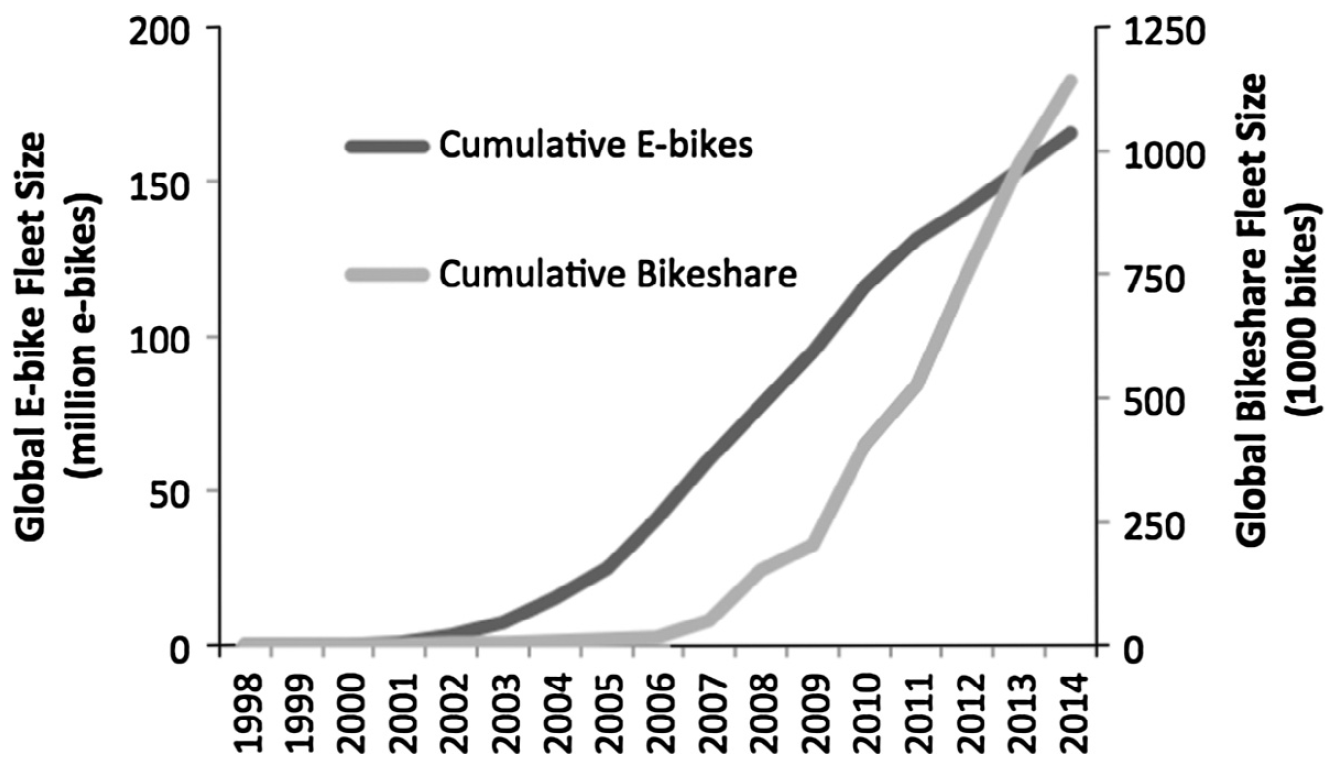
\includegraphics[width=0.6\linewidth]{image/bike_sharing} \caption{Growth in personal e-bike and public bikeshare systems (Campbell et al., 2016)}\label{fig:unnamed-chunk-7}
\end{figure}

Private BSS operators from China (\emph{Mobike, Ofo}) and Shanghai (\emph{oBike}) are currently introducing large fleets of station-less rental bikes in cities worldwide. The roll-out, especially in European cities, has encountered problems as city governments have not been able to coordinate the introduction (Zademach and Musch, 2018). Many bikes have been found abandoned around the cities. In addition, there are fears in some cases that the private companies introduced the BSS with the sole reason of tapping into private user data (Schöffel et al., 2017).
Furthermore, the company Montreal introduced ``BIXI'', fixed, portable, solar-powered and modular stations. They are self-contained and the stations can be placed, moved and relocated to desired locations within 20 minutes. ``Mega'' docking stations are available for special events (Midgley, 2011).
The number of BSSs has grown to over 800 units worldwide (Fishman, 2016). The public-private partnership model has been the most widespread, and the implementation of BSSs has been possible in cities with limited public funds (Zademach and Musch, 2018).
In Austria, there are multiple companies currently offering bicycle or e-bicycle sharing services such as \emph{Citybike, Ofo or oBike}. Nevertheless, about a year after their launch, the Asian providers of stationless rental bikes in Vienna (start-ups \emph{Ofo} and \emph{oBike}) have been in retreat from the federal capital (Rachbauer, 2018b). This has been a result of strict rules with respect to stationless rental bikes in Vienna announced on 1st August 2018. A failure to comply with the rules resulted in the bikes being removed for a fee. Previously, the traffic road act (\emph{StVO}) allowed the placement of rental bikes in public spaces and the city lacked the means of action against the providers. With the help of a so-called local police ordinance, the city hall required that the bike-sharing companies pick up objectionable bikes on weekdays within four hours and at night and on weekends within twelve hours after notification. If they did not comply, the bikes were removed for a fee. In addition, administrative fines of up to 700 euros were possible. Moreover, a limit of maximum 1500 bicycles per provider was also set. Now, the bikes are given a number and each one has to be registered with the city. According to Blum, setting up several companies to circumvent the upper limit is not allowed. The rental companies themselves also have to meet certaine criteria, for instance, there must be a company headquarters in Vienna and a service hotline. \emph{Ofo} and \emph{oBike} already meet these requirements (Rachbauer, 2018d).
Across Austria the situation with rental bikes differs significantly, for example in Innsbruck, renatal bikes were first introduced in 2014 and and are succesfully opearting. Meanwhile, in Linz rental bike system has been approved in 2017 and the docking stations are currently under construction. Further, in Salzburg the S-Bike rental system is operating and linked to federal funding (Affenzeller, 2020, Citybike Salzburg, no date a). On the other hand in Graz there is no uniform bike rental system and these services are provided by shops and hotels (Rachbauer, 2016).

\hypertarget{relevant-initiatives-in-austria-9}{%
\subsection*{Relevant initiatives in Austria}\label{relevant-initiatives-in-austria-9}}
\addcontentsline{toc}{subsection}{Relevant initiatives in Austria}

\begin{itemize}
\tightlist
\item
  \href{https://www.citybikewien.at/de}{citybikewien}
\item
  \href{http://www.citybikesalzburg.at/}{citybikesalzburg}
\item
  \href{https://www.nextbike.at/de/niederoesterreich/}{nextbike}
\item
  \href{https://www.tips.at/nachrichten/linz/land-leute/523512-linzer-radverleih-startet-im-fruehjahr-an-40-standorten}{tpis.at}
\end{itemize}

\hypertarget{impacts-with-respect-to-sustainable-development-goals-sdgs-9}{%
\subsection*{Impacts with respect to Sustainable Development Goals (SDGs)}\label{impacts-with-respect-to-sustainable-development-goals-sdgs-9}}
\addcontentsline{toc}{subsection}{Impacts with respect to Sustainable Development Goals (SDGs)}

\begin{longtable}[]{@{}ccccc@{}}
\toprule
\begin{minipage}[b]{0.17\columnwidth}\centering
Impact level\strut
\end{minipage} & \begin{minipage}[b]{0.16\columnwidth}\centering
Indicator\strut
\end{minipage} & \begin{minipage}[b]{0.17\columnwidth}\centering
Impact direction\strut
\end{minipage} & \begin{minipage}[b]{0.17\columnwidth}\centering
Goal description and number\strut
\end{minipage} & \begin{minipage}[b]{0.17\columnwidth}\centering
Source\strut
\end{minipage}\tabularnewline
\midrule
\endhead
\begin{minipage}[t]{0.17\columnwidth}\centering
Individual\strut
\end{minipage} & \begin{minipage}[t]{0.16\columnwidth}\centering
Often first 30-60 minutes free of charge\strut
\end{minipage} & \begin{minipage}[t]{0.17\columnwidth}\centering
\textbf{+}\strut
\end{minipage} & \begin{minipage}[t]{0.17\columnwidth}\centering
Equality (\emph{5,10})\strut
\end{minipage} & \begin{minipage}[t]{0.17\columnwidth}\centering
Citybike Salzburg, no date b; Citybike Wien, no date; Nextbike Niederoesterreich, no date\strut
\end{minipage}\tabularnewline
\begin{minipage}[t]{0.17\columnwidth}\centering
Individual\strut
\end{minipage} & \begin{minipage}[t]{0.16\columnwidth}\centering
Continuous advancement in bike features\strut
\end{minipage} & \begin{minipage}[t]{0.17\columnwidth}\centering
\textbf{+}\strut
\end{minipage} & \begin{minipage}[t]{0.17\columnwidth}\centering
Innovation \& Infrastructure (\emph{9})\strut
\end{minipage} & \begin{minipage}[t]{0.17\columnwidth}\centering
Zademach \& Musch, 2018\strut
\end{minipage}\tabularnewline
\begin{minipage}[t]{0.17\columnwidth}\centering
Systemic\strut
\end{minipage} & \begin{minipage}[t]{0.16\columnwidth}\centering
Wider access to this cheap or free mobility service\strut
\end{minipage} & \begin{minipage}[t]{0.17\columnwidth}\centering
\textbf{+}\strut
\end{minipage} & \begin{minipage}[t]{0.17\columnwidth}\centering
Equality (\emph{5,10})\strut
\end{minipage} & \begin{minipage}[t]{0.17\columnwidth}\centering
El Arbi \& Stephane, 2020\strut
\end{minipage}\tabularnewline
\begin{minipage}[t]{0.17\columnwidth}\centering
Systemic\strut
\end{minipage} & \begin{minipage}[t]{0.16\columnwidth}\centering
Air pollution, noise pollution and congestion reduced\strut
\end{minipage} & \begin{minipage}[t]{0.17\columnwidth}\centering
\textbf{+}\strut
\end{minipage} & \begin{minipage}[t]{0.17\columnwidth}\centering
Environmental sustainability (\emph{7,12,13,15})\strut
\end{minipage} & \begin{minipage}[t]{0.17\columnwidth}\centering
El Arbi \& Stephane, 2020\strut
\end{minipage}\tabularnewline
\begin{minipage}[t]{0.17\columnwidth}\centering
Systemic\strut
\end{minipage} & \begin{minipage}[t]{0.16\columnwidth}\centering
Investment in bike sharing infrastructure\strut
\end{minipage} & \begin{minipage}[t]{0.17\columnwidth}\centering
\textbf{+}\strut
\end{minipage} & \begin{minipage}[t]{0.17\columnwidth}\centering
Innovation \& Infrastructure (\emph{9})\strut
\end{minipage} & \begin{minipage}[t]{0.17\columnwidth}\centering
der Grazer, 2019; Hillebrand, 2019; Affenzeller, 2020; Tech \& Nature, 2020\strut
\end{minipage}\tabularnewline
\begin{minipage}[t]{0.17\columnwidth}\centering
Systemic\strut
\end{minipage} & \begin{minipage}[t]{0.16\columnwidth}\centering
48\% of all systems are operated as public-private partnerships\strut
\end{minipage} & \begin{minipage}[t]{0.17\columnwidth}\centering
\textbf{+}\strut
\end{minipage} & \begin{minipage}[t]{0.17\columnwidth}\centering
Partnership \& collaborations (\emph{17})\strut
\end{minipage} & \begin{minipage}[t]{0.17\columnwidth}\centering
Midgley, 2011\strut
\end{minipage}\tabularnewline
\bottomrule
\end{longtable}

\hypertarget{technology-and-societal-readiness-level-9}{%
\subsection*{Technology and societal readiness level}\label{technology-and-societal-readiness-level-9}}
\addcontentsline{toc}{subsection}{Technology and societal readiness level}

\begin{longtable}[]{@{}cc@{}}
\toprule
TRL & SRL\tabularnewline
\midrule
\endhead
7-9 & 5-7\tabularnewline
\bottomrule
\end{longtable}

\hypertarget{open-questions-9}{%
\subsection*{Open questions}\label{open-questions-9}}
\addcontentsline{toc}{subsection}{Open questions}

\begin{enumerate}
\def\labelenumi{\arabic{enumi}.}
\tightlist
\item
  What measures can be implemented to tackle the vandalism of the bikes?
\item
  Which bike system (docked vs.~free-floating) is more sustainable in the long-term?
\end{enumerate}

\hypertarget{further-links-6}{%
\subsection*{Further links}\label{further-links-6}}
\addcontentsline{toc}{subsection}{Further links}

\begin{itemize}
\tightlist
\item
  \href{http://en.cyclocity.com/}{cyclocity.com}
\end{itemize}

\hypertarget{references-9}{%
\subsection*{References}\label{references-9}}
\addcontentsline{toc}{subsection}{References}

\begin{itemize}
\tightlist
\item
  Affenzeller, J. (2020) Linzer Radverleih startet im Frühjahr an 40 Standorten. Available at: \url{https://www.tips.at/nachrichten/linz/land-leute/523512-linzer-radverleih-startet-im-fruehjahr-an-40-standorten} (Accessed: 18 January 2021).
\item
  El Arbi, A. A. and Stephane, C. K. T. (2020) `Intelligent Management of Bike Sharing in Smart Cities using Machine Learning and Internet of Things', Sustainable Cities and Society. Elsevier B.V., p.~135907. doi: 10.1016/j.scs.2020.102702.
\item
  Campbell, A. A. et al.~(2016) `Factors influencing the choice of shared bicycles and shared electric bikes in Beijing', Transportation Research Part C: Emerging Technologies. Elsevier Ltd, 67, pp.~399--414. doi: 10.1016/j.trc.2016.03.004.
\item
  Cheng, L. et al.~(2020) `How could the station-based bike sharing system and the free-floating bike sharing system be coordinated?', Journal of Transport Geography. Elsevier Ltd, 89(March 2019), p.~102896. doi: 10.1016/j.jtrangeo.2020.102896.
\item
  Cheng, X. and Gao, Y. (2018) `The Optimal Monthly Strategy Pricing of Free-Floating Bike Sharing Platform', Modern Economy. Scientific Research Publishing, Inc, 09(02), pp.~318--338. doi: 10.4236/me.2018.92021.
\item
  Citybike Salzburg (no date a) Citybike Salzburg. Available at: \url{http://www.citybikesalzburg.at/hanuschplatz.php} (Accessed: 12 January 2021).
\item
  Citybike Salzburg (no date b) Citybike Salzburg - Tarife. Available at: \url{http://www.citybikesalzburg.at/tarife.php} (Accessed: 18 January 2021).
\item
  Citybike Wien (2019) 10 Millionen Fahrten bei Citybike Wien! Available at: \url{https://www.citybikewien.at/de/news/595-neuer-meilenstein-bei-citybike-wien-erreicht} (Accessed: 12 January 2021).
\item
  Citybike Wien (no date) Tarife - Citybike Wien. Available at: \url{https://www.citybikewien.at/de/tarife} (Accessed: 18 January 2021).
\item
  DeMaio, P. (2009) `Bike-sharing: History, Impacts, Models of Provision, and Future', Journal of Public Transportation. University of South Florida Libraries, 12(4), pp.~41--56. doi: 10.5038/2375-0901.12.4.3.
\item
  Eillie, A. (2016) Oxford Test Drives Peer-to-Peer Bike Sharing. Available at: \url{https://www.bloomberg.com/news/articles/2016-09-13/cycle-land-is-a-new-peer-to-peer-bike-sharing-platform} (Accessed: 8 January 2021).
\item
  Fishman, E. et al.~(2014) `Barriers to bikesharing: An analysis from Melbourne and Brisbane', Journal of Transport Geography. Elsevier Ltd, 41, pp.~325--337. doi: 10.1016/j.jtrangeo.2014.08.005.
\item
  Fishman, E. (2016) `Bikeshare: A Review of Recent Literature', Transport Reviews. Routledge, 36(1), pp.~92--113. doi: 10.1080/01441647.2015.1033036.
\item
  der Grazer (2019) 100 Millionen Euro für Fahrrad-Offensive im Großraum Graz -- Der Grazer. Available at: \url{https://grazer.at/de/uHAnk5t2/100-millionen-euro-fuer-fahrrad-offensive-im-graz/} (Accessed: 18 January 2021).
\item
  Gu, T., Kim, I. and Currie, G. (2019) `To be or not to be dockless: Empirical analysis of dockless bikeshare development in China', Transportation Research Part A: Policy and Practice. Elsevier Ltd, 119, pp.~122--147. doi: 10.1016/j.tra.2018.11.007.
\item
  Hillebrand, T. (2019) Mietradsystem `Stadtrad Innsbruck' - VCÖ Vorbildhafte Mobilitätsprojekte. Available at: \url{https://mobilitaetsprojekte.vcoe.at/mietradsystem-stadtrad-innsbruck-2019} (Accessed: 18 January 2021).
\item
  Li, H. et al.~(2019) `Effects of dockless bike-sharing systems on the usage of the London Cycle Hire', Transportation Research Part A: Policy and Practice. Elsevier Ltd, 130, pp.~398--411. doi: 10.1016/j.tra.2019.09.050.
\item
  Ma, X. et al.~(2020) `A comparison in travel patterns and determinants of user demand between docked and dockless bike-sharing systems using multi-sourced data', Transportation Research Part A: Policy and Practice. Elsevier, 139(June), pp.~148--173. doi: 10.1016/j.tra.2020.06.022.
\item
  Midgley, P. (2011) `Bicycle-Sharing Schemes: Enhancing Sustainable Mobility in Urban Areas', Commission on Sustainable Development, Nine teent(8), p.~24. Available at: \url{http://www.un.org/esa/dsd/resources/res_pdfs/csd-19/Background-Paper8-P.Midgley-Bicycle.pdf}.
\item
  Nextbike Niederösterreich (no date) Nextbike Niederösterreich - Tarife. Available at: \url{https://www.nextbike.at/de/niederoesterreich/preise/} (Accessed: 18 January 2021).
\item
  Rachbauer, S. (2016) Bikesharing in Österreich: Leihräder auf der Überholspur \textbar{} kurier.at. Available at: \url{https://kurier.at/chronik/oesterreich/bikesharing-in-oesterreich-leihraeder-auf-der-ueberholspur/400067369} (Accessed: 12 January 2021).
\item
  Rachbauer, S. (2018a) Bikesharing in Österreich: Leihräder auf der Überholspur. Available at: \url{https://kurier.at/chronik/oesterreich/bikesharing-in-oesterreich-leihraeder-auf-der-ueberholspur/400067369}.
\item
  Rachbauer, S. (2018b) Leihräder: Wiener wollen es aufgeräumt. Available at: \url{https://kurier.at/chronik/wien/leihraeder-wiener-wollen-es-aufgeraeumt/400067357} (Accessed: 12 January 2021).
\item
  Rachbauer, S. (2018c) Leihräder: Wiener wollen es aufgeräumt. Available at: \url{https://kurier.at/chronik/wien/leihraeder-wiener-wollen-es-aufgeraeumt/400067357}.
\item
  Rachbauer, S. (2018d) Wien führt strenge Regeln für stationslose Leihräder ein. Available at: \url{https://kurier.at/chronik/wien/wien-fuehrt-strenge-regeln-fuer-stationslose-leihraeder-ein/312.944.617} (Accessed: 12 January 2021).
\item
  Schöffel, R., Zierer, M. and Kühne, S. (2017) Nutzerdaten offen im Netz: BR deckt Datenleck beim Fahrradverleiher Obike auf. Available at: \url{https://www.br.de/nachricht/datenleck-obike-100.html} (Accessed: 8 January 2021).
\item
  Sun, S. and Ertz, M. (2021) `Contribution of bike-sharing to urban resource conservation: The case of free-floating bike-sharing', Journal of Cleaner Production. Elsevier Ltd, 280, p.~124416. doi: 10.1016/j.jclepro.2020.124416.
\item
  Tech \& Nature (2020) Niederösterreich modernisiert Sharing-Bike-Flotte `nextbike' - Tech \& Nature. Available at: \url{https://www.techandnature.com/niederosterreich-modernisiert-sharing-bike-flotte-nextbike/} (Accessed: 18 January 2021).
\item
  Zademach, H. M. and Musch, A. K. (2018) `Bicycle-sharing systems in an alternative/diverse economy perspective: a sympathetic critique', Local Environment. Taylor \& Francis, 23(7), pp.~734--746. doi: 10.1080/13549839.2018.1434494.
\item
  Zhang, Y., Lin, D. and Mi, Z. (2019) `Electric fence planning for dockless bike-sharing services', Journal of Cleaner Production, 206, pp.~383--393. doi: 10.1016/j.jclepro.2018.09.215.
\end{itemize}

\hypertarget{e-scooters}{%
\section{E-scooters}\label{e-scooters}}

\hypertarget{synonyms-10}{%
\subsection*{Synonyms}\label{synonyms-10}}
\addcontentsline{toc}{subsection}{Synonyms}

\emph{electric scooter}

\hypertarget{definition-10}{%
\subsection*{Definition}\label{definition-10}}
\addcontentsline{toc}{subsection}{Definition}

E-scooters are electrically powered scooters which move at a similar speed to bicycles. They are one of micro-mobility solutions which is growing trend in urban mobility. It encompasses all human-powered micro-vehicles, such as bicycles and scooters, but also new micro-vehicles such as e-scooters, e-bikes and some other small, electrically powered vehicles (Oeschger, Carroll and Caulfield, 2020). Most of the modern vehicles of this type are available for both shared and private use and are gaining wide acceptance.
E-scooters have promised a solution to the last mile problem since their introduction in 2017 (Siegfried et al, 2021). They are seen as alternatives to cars and provide potential for reducing traffic congestion, noise and pollution. Initial results suggest that e-scooters are mainly used for distances between 1 and 6 km. Empirical evidence shows that e-scooters can substitute walking rather than driving for these short distances (James et al., 2019; Portland Bureau of Transportation, 2019). In addition to the potential positive environmental impact of e-scooters on the transportation system, some safety concerns have been raised. Most e-scooter users who had an accident have ridden without a helmet (Liew et al, 2020). In general, e-scooters are almost exclusively issued without protective equipment (Allem and Majmundar, 2019). The safety issues do not only affect the riders themselves, but also have an impact on other road users, especially pedestrians (Sikka et al., 2019). It has even been criticised that technology follows the idea of ``sell first, safety later'' (Choron and Sakran, 2019).

\hypertarget{key-stakeholders-10}{%
\subsection*{Key stakeholders}\label{key-stakeholders-10}}
\addcontentsline{toc}{subsection}{Key stakeholders}

\begin{itemize}
\tightlist
\item
  \textbf{Affected}: Mobile citizens, pedestrians, insurers
\item
  \textbf{Responsible}: National governments, city government, private Companies
\end{itemize}

\hypertarget{current-state-of-art-in-research-10}{%
\subsection*{Current state of art in research}\label{current-state-of-art-in-research-10}}
\addcontentsline{toc}{subsection}{Current state of art in research}

Since e-scooters are already well-established technology, most research focuses on safety and accidents, user behaviour and potential environmental impact of uptake of this micro-mobility option. Some studies advocate e-scooters as an environmentally friendly solution for crowded cities, others report contradictory results and point to safety issues.
Moreover, research also explores whether the presence of e-scooters reduces bicycle thefts (Gössling, 2020). In Gothenburg, Sweden, the police reported that the number of bicycle thefts halved after the introduction of e-scooters and rental bikes (Sydsvenskan, 2019).

\hypertarget{current-state-of-art-in-practice-10}{%
\subsection*{Current state of art in practice}\label{current-state-of-art-in-practice-10}}
\addcontentsline{toc}{subsection}{Current state of art in practice}

E-scooter providers such as \emph{Lime} and \emph{Bird}, which launched operations in California in 2017, can now be found in over 100 cities worldwide and have since recorded millions of rides. E-scooter provider \emph{VOI} has experienced similar growth in Europe and entered the market in 10 countries in just one year after launching in Sweden and has recorded over 16 million rides (Oeschger et al., 2020). The results of a survey indicate that e-scooters are primarily seen as entertainment and not as a means of transport (Siegfried et al., 2021).
Maximum speed limits are an important issue and internationally there are different approaches. Los Angeles and Dallas, for example, have no speed limit, as far as can be deduced from the news; while the limit in Vienna is 25 km/h (Schwarz, 2019). Paris is discussing reducing the speed limit to 20 km/h on cycle paths and 8 km/h in parks and pedestrian areas (Négroni, 2019). One problem with the maximum speeds is that some of the e-scooter models can go much faster than 25 km/h (Le Figaro, 2018). To counteract the negative consequences of the introduction of e-scooters, cities have evaluated and implemented various rules and guidelines. Media analysis suggests that the city councils should introduce the following rules as a minimal requirement: speed limits, restrictions on the exclusive use of bicycle infrastructure and a designation of parking spaces for rental and return. Behavioural campaigns and fines, are needed to limit negative consequences of e-scooter use (Gössling, 2020).
In Vienna, only very few e-scooters are used on bicycle paths (between 4.9\% and 7.1\% compared to other bicycle path users). Given the modal split of Vienna (7\% cycling), it can be concluded that e-scooters do not yet have a significant role in Vienna's transport system (Laa and Leth, 2020).

\hypertarget{relevant-initiatives-in-austria-10}{%
\subsection*{Relevant initiatives in Austria}\label{relevant-initiatives-in-austria-10}}
\addcontentsline{toc}{subsection}{Relevant initiatives in Austria}

\begin{itemize}
\tightlist
\item
  \href{https://autorevue.at/ratgeber/e-scooter-wien-vergleich}{autorevue.at}
\item
  \href{https://www.stadt-wien.at/wien/news/e-scooter-sharing-system-in-wien.html}{stadt-wien.at}
\item
  \href{https://www.wien.gv.at/verkehr/scooter-roller/index.html}{wien.gv.at}
\item
  \href{https://www.oeamtc.at/thema/fahrrad/e-kleintretroller-e-scooter-in-oesterreich-31721872}{oeamtc.at}
\item
  \href{https://www.oesterreich.gv.at/themen/freizeit_und_strassenverkehr/Elektro-Scooter,-Quads-und-Co/Seite.610110.html}{oesterreich.gv.at}
\end{itemize}

\hypertarget{impacts-with-respect-to-sustainable-development-goals-sdgs-10}{%
\subsection*{Impacts with respect to Sustainable Development Goals (SDGs)}\label{impacts-with-respect-to-sustainable-development-goals-sdgs-10}}
\addcontentsline{toc}{subsection}{Impacts with respect to Sustainable Development Goals (SDGs)}

\begin{longtable}[]{@{}ccccc@{}}
\toprule
\begin{minipage}[b]{0.17\columnwidth}\centering
Impact level\strut
\end{minipage} & \begin{minipage}[b]{0.16\columnwidth}\centering
Indicator\strut
\end{minipage} & \begin{minipage}[b]{0.17\columnwidth}\centering
Impact direction\strut
\end{minipage} & \begin{minipage}[b]{0.17\columnwidth}\centering
Goal description and number\strut
\end{minipage} & \begin{minipage}[b]{0.17\columnwidth}\centering
Source\strut
\end{minipage}\tabularnewline
\midrule
\endhead
\begin{minipage}[t]{0.17\columnwidth}\centering
Individual\strut
\end{minipage} & \begin{minipage}[t]{0.16\columnwidth}\centering
E-scooter trips replace mainly walking trips\strut
\end{minipage} & \begin{minipage}[t]{0.17\columnwidth}\centering
\textbf{-}\strut
\end{minipage} & \begin{minipage}[t]{0.17\columnwidth}\centering
Health \& Wellbeing (\emph{3})\strut
\end{minipage} & \begin{minipage}[t]{0.17\columnwidth}\centering
Laa \& Leth, 2020\strut
\end{minipage}\tabularnewline
\begin{minipage}[t]{0.17\columnwidth}\centering
Individual\strut
\end{minipage} & \begin{minipage}[t]{0.16\columnwidth}\centering
More expensive compared to public transport\strut
\end{minipage} & \begin{minipage}[t]{0.17\columnwidth}\centering
\textbf{-}\strut
\end{minipage} & \begin{minipage}[t]{0.17\columnwidth}\centering
Sustainable economic development (\emph{8,11})\strut
\end{minipage} & \begin{minipage}[t]{0.17\columnwidth}\centering
Widholm, 2021; Wiener Linien, 2021\strut
\end{minipage}\tabularnewline
\begin{minipage}[t]{0.17\columnwidth}\centering
Individual\strut
\end{minipage} & \begin{minipage}[t]{0.16\columnwidth}\centering
Increase in participants on existing road infrastructure\strut
\end{minipage} & \begin{minipage}[t]{0.17\columnwidth}\centering
\textbf{\textasciitilde{}}\strut
\end{minipage} & \begin{minipage}[t]{0.17\columnwidth}\centering
Innovation \& Infrastructure (\emph{9})\strut
\end{minipage} & \begin{minipage}[t]{0.17\columnwidth}\centering
Laa \& Leth, 2020\strut
\end{minipage}\tabularnewline
\begin{minipage}[t]{0.17\columnwidth}\centering
Systemic\strut
\end{minipage} & \begin{minipage}[t]{0.16\columnwidth}\centering
Highest user share among young males\strut
\end{minipage} & \begin{minipage}[t]{0.17\columnwidth}\centering
\textbf{-}\strut
\end{minipage} & \begin{minipage}[t]{0.17\columnwidth}\centering
Equality (\emph{5,10})\strut
\end{minipage} & \begin{minipage}[t]{0.17\columnwidth}\centering
Laa \& Leth, 2020\strut
\end{minipage}\tabularnewline
\begin{minipage}[t]{0.17\columnwidth}\centering
Systemic\strut
\end{minipage} & \begin{minipage}[t]{0.16\columnwidth}\centering
E-scooter trips repalce more sustainable transport modes\strut
\end{minipage} & \begin{minipage}[t]{0.17\columnwidth}\centering
\textbf{-}\strut
\end{minipage} & \begin{minipage}[t]{0.17\columnwidth}\centering
Environmental sustainability (\emph{7,12,13,15})\strut
\end{minipage} & \begin{minipage}[t]{0.17\columnwidth}\centering
Laa \& Leth, 2020\strut
\end{minipage}\tabularnewline
\begin{minipage}[t]{0.17\columnwidth}\centering
Systemic\strut
\end{minipage} & \begin{minipage}[t]{0.16\columnwidth}\centering
Growth in micromobility sector\strut
\end{minipage} & \begin{minipage}[t]{0.17\columnwidth}\centering
\textbf{+}\strut
\end{minipage} & \begin{minipage}[t]{0.17\columnwidth}\centering
Sustainable economic development (\emph{8,11})\strut
\end{minipage} & \begin{minipage}[t]{0.17\columnwidth}\centering
Goessling, 2020\strut
\end{minipage}\tabularnewline
\bottomrule
\end{longtable}

\hypertarget{technology-and-societal-readiness-level-10}{%
\subsection*{Technology and societal readiness level}\label{technology-and-societal-readiness-level-10}}
\addcontentsline{toc}{subsection}{Technology and societal readiness level}

\begin{longtable}[]{@{}cc@{}}
\toprule
TRL & SRL\tabularnewline
\midrule
\endhead
7-9 & 7-9\tabularnewline
\bottomrule
\end{longtable}

\hypertarget{open-questions-10}{%
\subsection*{Open questions}\label{open-questions-10}}
\addcontentsline{toc}{subsection}{Open questions}

\begin{enumerate}
\def\labelenumi{\arabic{enumi}.}
\tightlist
\item
  Will an increasing presence of e-scooters on the bicycle infrastructure or in pedestrian zones require separate solution in urban road infrastructure?
\end{enumerate}

\hypertarget{references-10}{%
\subsection*{References}\label{references-10}}
\addcontentsline{toc}{subsection}{References}

\begin{itemize}
\tightlist
\item
  Allem, J. P. and Majmundar, A. (2019) `Are electric scooters promoted on social media with safety in mind? A case study on Bird's Instagram', Preventive Medicine Reports. Elsevier Inc., pp.~62--63. doi: 10.1016/j.pmedr.2018.11.013.
\item
  Choron, R. L. and Sakran, J. V. (2019) `The Integration of Electric Scooters: Useful Technology or Public Health Problem?', American journal of public health. NLM (Medline), 109(4), pp.~555--556. doi: 10.2105/AJPH.2019.304955.
\item
  Le Figaro (2018) `Trottinettes: la mairie de Paris veut une réglementation nationale', 9 September. Available at: \url{https://www.lefigaro.fr/flash-eco/2018/09/09/97002-20180909FILWWW00064-trottinettes-la-mairie-de-paris-veut-une-reglementation-nationale.php} (Accessed: 20 January 2021).
\item
  Gössling, S. (2020) `Integrating e-scooters in urban transportation: Problems, policies, and the prospect of system change', Transportation Research Part D: Transport and Environment. Elsevier, 79(January), p.~102230. doi: 10.1016/j.trd.2020.102230.
  James, O. et al.~(2019) `Pedestrians and E-Scooters: An Initial Look at E-Scooter Parking and Perceptions by Riders and Non-Riders', Sustainability. MDPI AG, 11(20), p.~5591. doi: 10.3390/su11205591.
  Laa, B. and Leth, U. (2020) `Survey of E-scooter users in Vienna: Who they are and how they ride', Journal of Transport Geography. Elsevier, 89(October), p.~102874. doi: 10.1016/j.jtrangeo.2020.102874.
\item
  Liew, Y. K., Wee, C. P. J. and Pek, J. H. (2020) `New peril on our roads: A retrospective study of electric scooter-related injuries', Singapore Medical Journal. Singapore Medical Association, 61(2), pp.~92--95. doi: 10.11622/smedj.2019083.
\item
  Négroni, A. (2019) `Paris: Hidalgo prend des mesures contre les trottinettes électriques', 6 June. Available at: \url{https://www.lefigaro.fr/actualite-france/trottinettes-paris-prend-des-mesures-20190606} (Accessed: 20 January 2021).
\item
  OECD/ITF (2020) `Safe Micromobility', p.~98. Available at: \url{https://www.itf-oecd.org/safe-micromobility}.
\item
  Oeschger, G., Carroll, P. and Caulfield, B. (2020) `Micromobility and public transport integration: The current state of knowledge', Transportation Research Part D: Transport and Environment. Elsevier Ltd, 89, p.~102628. doi: 10.1016/j.trd.2020.102628.
\item
  Portland Bureau of Transportation (2019) 2018 E-Scooter Findings Report. Available at: \url{https://www.portlandoregon.gov/transportation/article/709719\%0Ahttps://trid.trb.org/view/1607260}.
\item
  Schwarz, R. (2019) E-Bikes und E-Scooter sind viel zu schnell! - Ideen-Blog - derStandard.at › Diskurs. Available at: \url{https://www.derstandard.at/story/2000106514149/e-bikes-und-e-scooter-sind-viel-zu-schnell} (Accessed: 20 January 2021).
\item
  Siegfried, C., Martin, B. and Reichenberger, Y. (2021) `Consumer acceptance of shared e-scooters for urban and short-distance mobility', Transportation Research Part D. Elsevier Ltd, 91(January), p.~102680. doi: 10.1016/j.trd.2020.102680.
\item
  Sikka, N. et al.~(2019) `Sharing the sidewalk: A case of E-scooter related pedestrian injury', American Journal of Emergency Medicine. W.B. Saunders, 37(9), pp.~1807.e5-1807.e7. doi: 10.1016/j.ajem.2019.06.017.
\item
  Sydsvenskan (2019) Elsparkcyklarna minskar cykelstölderna - Sydsvenskan. Available at: \url{https://www.sydsvenskan.se/2019-08-30/elsparkcyklarna-minskar-cykelstolderna} (Accessed: 20 January 2021).
\item
  Widholm, K. (2021) E-Scooter Sharing-System: Roller von Lime, Tier, Bird und Co.~Available at: \url{https://www.stadt-wien.at/wien/news/e-scooter-sharing-system-in-wien.html} (Accessed: 20 January 2021).
\item
  Wiener Linien (2021) Übersicht Tickets \textbar{} Tickets \textbar{} Fahrgastinfo \textbar{} Wiener Linien. Available at: \url{https://www.wienerlinien.at/eportal3/ep/channelView.do/pageTypeId/66526/channelId/-46648} (Accessed: 20 January 2021).
\item
  Zagorskas, J. and Burinskiene, M. (2020) `Challenges caused by increased use of E-powered personal mobility vehicles in European cities', Sustainability (Switzerland). MDPI AG, 12(1), p.~273. doi: 10.3390/su12010273.
\end{itemize}

\hypertarget{ride-hailing}{%
\section{Ride-hailing}\label{ride-hailing}}

\hypertarget{alternative}{%
\chapter{Alternative power sources}\label{alternative}}

\hypertarget{hydrogen-fuel-cell}{%
\section{Hydrogen fuel cell}\label{hydrogen-fuel-cell}}

\hypertarget{definition-11}{%
\subsection*{Definition}\label{definition-11}}
\addcontentsline{toc}{subsection}{Definition}

Hydrogen Fuel Cells are systems that use hydrogen as fuel to generate electrical energy in a Fuel Cell and drive the vehicle with electrical structure. In a technical manner, they show similarities with electric vehicles. The advantages of Fuel Cell Electrical Vehicles (FCEV) are emission-free (water only), fast refuelling, noiseless driving, more economical fuel consumption and efficiency, easy maintenance. Regardless of these benefits, FCEV has some disadvantages, such as limited range, lack of hydrogen refuelling stations, safety problems, low profitability for car manufacturers, high prices and lower awareness and acceptance (Tanç et al., 2019; Borgstedt et al., 2017; Iribarren et al., 2016). Moreover, FCEVs have higher energy density than electric batteries which enables them to drive further with heavier loads. At the same time, it raises constraints on weight and size of the energy storage in the vehicles. Consequently, FCEVs are more suitable for freight transport, commercial vehicles, buses, trains, ships and aircrafts, where the performance requirements are higher. Prototypes of all the examples mentioned already exist (Eichlseder et al, 2018). In terms of private cars, the FCEVs are likely to provide advantage for long-distance travelling (Roadmap Europe, 2019).

\hypertarget{key-stakeholders-11}{%
\subsection*{Key stakeholders}\label{key-stakeholders-11}}
\addcontentsline{toc}{subsection}{Key stakeholders}

\begin{itemize}
\tightlist
\item
  \textbf{Affected}: Conventional Cars' Drivers, Citizen
\item
  \textbf{Responsible}: National Governments, Car Manufacturers, International lobbyists, Private Companies
\end{itemize}

\hypertarget{current-state-of-art-in-research-11}{%
\subsection*{Current state of art in research}\label{current-state-of-art-in-research-11}}
\addcontentsline{toc}{subsection}{Current state of art in research}

The goal of alternative propulsion systems is to minimize or eliminate completely the climate-damaging CO\textsubscript{2} emissions, consequently the European Community Research Program proposes electromobility as a priority research area. In particular, the most substantial research is carried out on methods of hydrogen production using biological and photochemical processes because 95\% of hydrogen currently produced on an industrial scale comes from fossil hydrocarbons and only 5\% from water by electrolysis. Where the only emission-free production process of hydrogen is the electrochemical water splitting in electrolysis, when the required electricity is generated from wind-, water or solar energy. This process results in high degrees of purity and usually achieves efficiencies of up to 85\% (Eichlseder et al., 2018). Moreover, the electric vehicle policy aims at technology optimization, market development, durability and capacity of the batteries and charging stations (Alvarez-Meaza et al., 2020).

\hypertarget{current-state-of-art-in-practice-11}{%
\subsection*{Current state of art in practice}\label{current-state-of-art-in-practice-11}}
\addcontentsline{toc}{subsection}{Current state of art in practice}

Hydrogen in transport is only at the beginning of its development (in 2013 the first light FCEVs were introduced for leasing only). Compared to other alternative propulsion systems such as battery electric vehicles (BEVs), which were introduced to the vehicle market earlier, FCEVs show a similar upward trend. At the end of 2017, the total number of FCEVs in Europe reached 799 vehicles, of which 602 were passenger cars and 197 light commercial vehicles, while the total number of BEVs reached 447,150 vehicles. At the end of 2018, the number of FCEVs in Europe rose to about 1,110 (Apostolou and Xydis, 2019).
At the end of October 2019, 41 fuel cell passenger cars were registered in Austria. Worldwide, about 12,900 fuel cell vehicles were in operation at the end of 2018, 11,200 of them passenger cars. 46 percent of the vehicles are on the road in the USA, 43 percent in Asia and 11 percent in the EU (1,110 cars). In terms of commercial vehicles, China dominates with over 400 buses, followed by the USA with 55 and the EU with around 80 (Eichlseder et al., 2018).
In terms of the number of hydrogen refuelling stations (HRS) worldwide, just about 375 stations are in operation today, compared to 320 in 2017. Most of these are publicly available, the rest are demonstration/research projects and are used to supply hydrogen to private fleets. At the end of 2018, Europe was the region with the most HRS in operation with more than 170 HRS, while Asia (mainly Japan) was second with about 130 HRS and America (mainly the US) third with more than 70 stations installed. Figure below shows the number of HRS by country at the end of 2018 (Apostolou and Xydis, 2019):

\begin{figure}
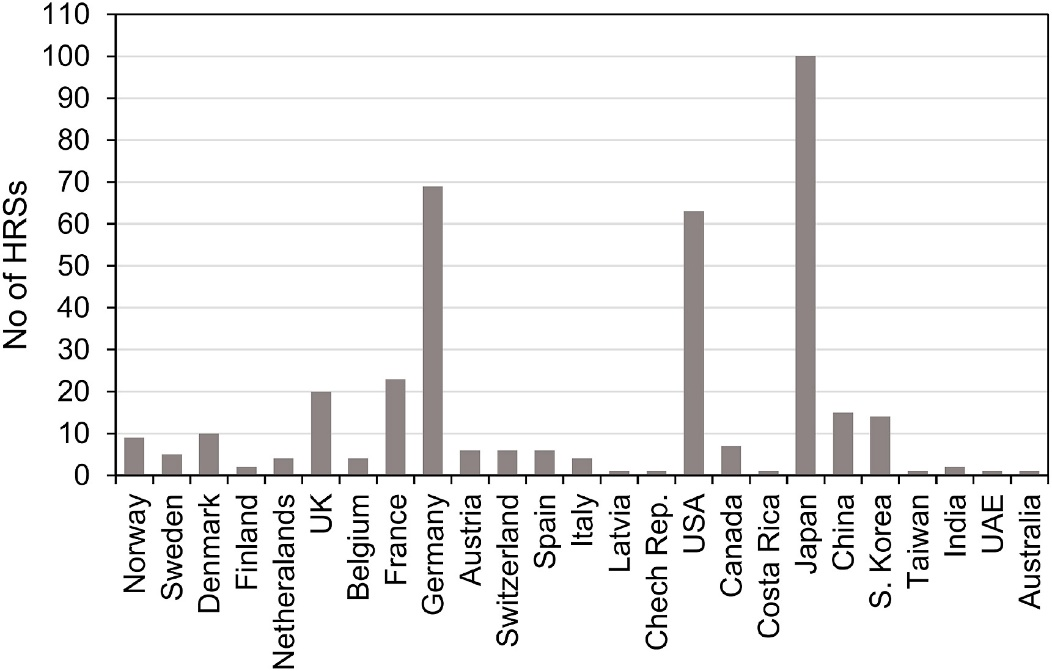
\includegraphics[width=0.6\linewidth]{image/hydrogen_refuel} \caption{Number of hydrogen refuelling stations worldwide (Apostolou and Xydis, 2019)}\label{fig:unnamed-chunk-8}
\end{figure}

The European Strategic Energy Technology Plan proposes hydrogen and fuel-cell technologies as crucial for obtaining green-house gases reduction goals by 2050 (Roadmap Europe H., 2019; Alvarez-Meaza et al., 2020).

\hypertarget{relevant-initiatives-in-austria-11}{%
\subsection*{Relevant initiatives in Austria}\label{relevant-initiatives-in-austria-11}}
\addcontentsline{toc}{subsection}{Relevant initiatives in Austria}

\begin{itemize}
\tightlist
\item
  \href{https://fuelcellsworks.com/news/alstoms-hydrogen-train-successfully-completes-three-months-of-testing-in-austria/\#:~:text=Alstom's\%20Hydrogen\%20Train\%20Successfully\%20Completes\%20Three\%20Months\%20of\%20Testing\%20in\%20Austria,-By\%20FuelCellsWorksDecember\&text=Alstom's\%20Coradia\%20iLint\%2C\%20the\%20world's,Austrian\%20Federal\%20Railways}{hydrogen train}
\end{itemize}

\hypertarget{impacts-with-respect-to-sustainable-development-goals-sdgs-11}{%
\subsection*{Impacts with respect to Sustainable Development Goals (SDGs)}\label{impacts-with-respect-to-sustainable-development-goals-sdgs-11}}
\addcontentsline{toc}{subsection}{Impacts with respect to Sustainable Development Goals (SDGs)}

\begin{longtable}[]{@{}ccccc@{}}
\toprule
\begin{minipage}[b]{0.17\columnwidth}\centering
Impact level\strut
\end{minipage} & \begin{minipage}[b]{0.16\columnwidth}\centering
Indicator\strut
\end{minipage} & \begin{minipage}[b]{0.17\columnwidth}\centering
Impact direction\strut
\end{minipage} & \begin{minipage}[b]{0.17\columnwidth}\centering
Goal description and number\strut
\end{minipage} & \begin{minipage}[b]{0.17\columnwidth}\centering
Source\strut
\end{minipage}\tabularnewline
\midrule
\endhead
\begin{minipage}[t]{0.17\columnwidth}\centering
Individual\strut
\end{minipage} & \begin{minipage}[t]{0.16\columnwidth}\centering
Improved air quality\strut
\end{minipage} & \begin{minipage}[t]{0.17\columnwidth}\centering
\textbf{+}\strut
\end{minipage} & \begin{minipage}[t]{0.17\columnwidth}\centering
Health \& Wellbeing (\emph{3})\strut
\end{minipage} & \begin{minipage}[t]{0.17\columnwidth}\centering
Colella, Jacobson and Golden, 2005\strut
\end{minipage}\tabularnewline
\begin{minipage}[t]{0.17\columnwidth}\centering
Individual\strut
\end{minipage} & \begin{minipage}[t]{0.16\columnwidth}\centering
High prices of hydrogen cars and hydrogen fuel\strut
\end{minipage} & \begin{minipage}[t]{0.17\columnwidth}\centering
\textbf{-}\strut
\end{minipage} & \begin{minipage}[t]{0.17\columnwidth}\centering
Equality (\emph{5,10})\strut
\end{minipage} & \begin{minipage}[t]{0.17\columnwidth}\centering
Kanna and Paturu, 2020\strut
\end{minipage}\tabularnewline
\begin{minipage}[t]{0.17\columnwidth}\centering
Individual\strut
\end{minipage} & \begin{minipage}[t]{0.16\columnwidth}\centering
Cost for individuals\strut
\end{minipage} & \begin{minipage}[t]{0.17\columnwidth}\centering
\textbf{\textasciitilde{}}\strut
\end{minipage} & \begin{minipage}[t]{0.17\columnwidth}\centering
Sustainable economic development (\emph{8,11})\strut
\end{minipage} & \begin{minipage}[t]{0.17\columnwidth}\centering
Apostolou and Xydis, 2019\strut
\end{minipage}\tabularnewline
\begin{minipage}[t]{0.17\columnwidth}\centering
Systemic\strut
\end{minipage} & \begin{minipage}[t]{0.16\columnwidth}\centering
Emissions reduced, improved air quality\strut
\end{minipage} & \begin{minipage}[t]{0.17\columnwidth}\centering
\textbf{+}\strut
\end{minipage} & \begin{minipage}[t]{0.17\columnwidth}\centering
Health \& Wellbeing (\emph{3})\strut
\end{minipage} & \begin{minipage}[t]{0.17\columnwidth}\centering
Colella, Jacobson and Golden, 2005\strut
\end{minipage}\tabularnewline
\begin{minipage}[t]{0.17\columnwidth}\centering
Systemic\strut
\end{minipage} & \begin{minipage}[t]{0.16\columnwidth}\centering
Distribution and allocation of goods worsens\strut
\end{minipage} & \begin{minipage}[t]{0.17\columnwidth}\centering
\textbf{-}\strut
\end{minipage} & \begin{minipage}[t]{0.17\columnwidth}\centering
Equality (\emph{5,10})\strut
\end{minipage} & \begin{minipage}[t]{0.17\columnwidth}\centering
Kanna and Paturu, 2020\strut
\end{minipage}\tabularnewline
\begin{minipage}[t]{0.17\columnwidth}\centering
Systemic\strut
\end{minipage} & \begin{minipage}[t]{0.16\columnwidth}\centering
Reduced emissions, replacement of fossil fuels, energy transition\strut
\end{minipage} & \begin{minipage}[t]{0.17\columnwidth}\centering
\textbf{+}\strut
\end{minipage} & \begin{minipage}[t]{0.17\columnwidth}\centering
Environmental sustainability (\emph{7,12-13,15})\strut
\end{minipage} & \begin{minipage}[t]{0.17\columnwidth}\centering
Colella, Jacobson and Golden, 2005\strut
\end{minipage}\tabularnewline
\begin{minipage}[t]{0.17\columnwidth}\centering
Systemic\strut
\end{minipage} & \begin{minipage}[t]{0.16\columnwidth}\centering
Not yet profitable for manufacturers\strut
\end{minipage} & \begin{minipage}[t]{0.17\columnwidth}\centering
\textbf{+}\strut
\end{minipage} & \begin{minipage}[t]{0.17\columnwidth}\centering
Sustainable economic development (\emph{8,11})\strut
\end{minipage} & \begin{minipage}[t]{0.17\columnwidth}\centering
Roadmap Europe, 2019\strut
\end{minipage}\tabularnewline
\begin{minipage}[t]{0.17\columnwidth}\centering
Systemic\strut
\end{minipage} & \begin{minipage}[t]{0.16\columnwidth}\centering
Number of hydrogen refuelling stations increases\strut
\end{minipage} & \begin{minipage}[t]{0.17\columnwidth}\centering
\textbf{+}\strut
\end{minipage} & \begin{minipage}[t]{0.17\columnwidth}\centering
Innovation \& Infrastructure (\emph{9})\strut
\end{minipage} & \begin{minipage}[t]{0.17\columnwidth}\centering
Apostolou and Xydis, 2019\strut
\end{minipage}\tabularnewline
\begin{minipage}[t]{0.17\columnwidth}\centering
Systemic\strut
\end{minipage} & \begin{minipage}[t]{0.16\columnwidth}\centering
Sharing technologies internationally\strut
\end{minipage} & \begin{minipage}[t]{0.17\columnwidth}\centering
\textbf{+}\strut
\end{minipage} & \begin{minipage}[t]{0.17\columnwidth}\centering
Partnership \& collaborations (\emph{17})\strut
\end{minipage} & \begin{minipage}[t]{0.17\columnwidth}\centering
International Partnership for Hydrogen and Fuel Cells in the Economy, no date\strut
\end{minipage}\tabularnewline
\bottomrule
\end{longtable}

\hypertarget{technology-and-societal-readiness-level-11}{%
\subsection*{Technology and societal readiness level}\label{technology-and-societal-readiness-level-11}}
\addcontentsline{toc}{subsection}{Technology and societal readiness level}

\begin{longtable}[]{@{}cc@{}}
\toprule
TRL & SRL\tabularnewline
\midrule
\endhead
7-8 & 6-8\tabularnewline
\bottomrule
\end{longtable}

\hypertarget{open-questions-11}{%
\subsection*{Open questions}\label{open-questions-11}}
\addcontentsline{toc}{subsection}{Open questions}

\begin{enumerate}
\def\labelenumi{\arabic{enumi}.}
\tightlist
\item
  Who will drive the progress of hydrogen technology in heavy duty mobility in the future?
\item
  How to store large amounts of energy at low weight and in a restricted space within the vehicle? (Roadmap Europe, 2019)
\end{enumerate}

\hypertarget{further-links-7}{%
\subsection*{Further links}\label{further-links-7}}
\addcontentsline{toc}{subsection}{Further links}

\begin{itemize}
\tightlist
\item
  \href{https://www.europarl.europa.eu/news/nl/press-room/20180911IPR13114/more-electric-cars-on-eu-roads-by-2030}{europarlament}
\item
  \href{https://ec.europa.eu/transport/themes/urban/vehicles/road/hydrogen_en}{ec.europa}
\item
  \href{https://www.fch.europa.eu/news/hydrogen-roadmap-europe-sustainable-pathway-european-energy-transition}{fch.europa}
\end{itemize}

\hypertarget{references-11}{%
\subsection*{References}\label{references-11}}
\addcontentsline{toc}{subsection}{References}

\begin{itemize}
\tightlist
\item
  Alvarez-Meaza, I., Zarrabeitia-Bilbao, E., Rio-Belver, R. M., \& Garechana-Anacabe, G. (2020). Fuel-Cell Electric Vehicles: Plotting a Scientific and Technological Knowledge Map. Sustainability, 12(6), 2334.
\item
  Apostolou, D. and Xydis, G. (2019) `A literature review on hydrogen refuelling stations and infrastructure. Current status and future prospects', Renewable and Sustainable Energy Reviews. Elsevier Ltd, 113(May), p.~109292. doi: 10.1016/j.rser.2019.109292.
\item
  Borgstedt, P., Neyer, B., \& Schewe, G. (2017). Paving the road to electric vehicles--A patent analysis of the automotive supply industry. Journal of cleaner production, 167, 75-87.
\item
  Colella, W. G., Jacobson, M. Z. and Golden, D. M. (2005) `Switching to a U.S. hydrogen fuel cell vehicle fleet: The resultant change in emissions, energy use, and greenhouse gases', Journal of Power Sources, 150, pp.~150--181. doi: \url{https://doi.org/10.1016/j.jpowsour.2005.05.092}.
\item
  Doppelbauer, M. (2020) Grundlagen der Elektromobilität, Grundlagen der Elektromobilität. doi: 10.1007/978-3-658-29730-5.
\item
  Eichlseder, H., Klell, M. and Trattner, A. (2018) Wasserstoff in der Fahrzeugtechnik, Wasserstoff in der Fahrzeugtechnik. doi: 10.1007/978-3-8348-9674-2.
  International Partnership for Hydrogen and Fuel Cells in the Economy (no date) No Title. Available at: \url{https://www.iphe.net/}.
\item
  Iribarren, D., Martín-Gamboa, M., Manzano, J., \& Dufour, J. (2016). Assessing the social acceptance of hydrogen for transportation in Spain: an unintentional focus on target population for a potential hydrogen economy. International journal of hydrogen energy, 41(10), 5203-5208.
\item
  Kanna, I. V. and Paturu, P. (2020) `A study of hydrogen as an alternative fuel', International Journal of Ambient Energy. Taylor \& Francis, 41(12), pp.~1433--1436. doi: 10.1080/01430750.2018.1484803.
\item
  Lehmann, J. and Luschtinetz, T. (2014) Wasserstoff und Brennstoffzellen.
\item
  Pötscher, F. et al.~(2014) Ökobilanz alternativer Antriebe -- Elektrofahrzeuge im Vergleich.
\item
  Roadmap Europe (2019). A sustainable pathway for the European energy transition. Luxembourg: Publications Office of the European Union.
\item
  Schabbach, T. and Wesselak, V. (2020) Energie - Den Erneuerbaren gehört die Zukunft.
\item
  Tanç, B. et al.~(2019) `Overview of the next quarter century vision of hydrogen fuel cell electric vehicles', in International Journal of Hydrogen Energy, Volume 44, Issue 20, pp.~10120--10128.
\item
  Töpler, J. and Lehmann, J. (2017) Wasserstoff und Brennstoffzelle - Technologien und Marktkonzepte, Springer Vieweg.
\end{itemize}

\hypertarget{battery-electric}{%
\section{Battery electric}\label{battery-electric}}

\hypertarget{plugin-hybrid-vehicles}{%
\section{Plugin hybrid vehicles}\label{plugin-hybrid-vehicles}}

\hypertarget{synonyms-11}{%
\subsection*{Synonyms}\label{synonyms-11}}
\addcontentsline{toc}{subsection}{Synonyms}

\emph{Hybrid, HEV, PHEV}

\hypertarget{definition-12}{%
\subsection*{Definition}\label{definition-12}}
\addcontentsline{toc}{subsection}{Definition}

Plug-in hybrid vehicles effectively combine the electric drive with either a conventional combustion engine or other engines that use alternative fuels. This has the advantage that the vehicles can travel long distances, but consumption and emissions are reduced. An energy management system ensures that the optimum amount of energy is drawn from the two energy sources while driving. The ratio of energy consumption is influenced by the driving cycle. The faster the vehicle drives, the more energy is needed (Aswin and Senthilmurugan, 2018).

A hybrid vehicle is superior in terms of the reduced carbon footprint, better mileage than conventional vehicles, financial assistance for purchase, lower annual cost and a regenerative braking system. At the same time, the disadvantages include high purchasing cost, lower fuel efficiency because the extra parts installed take up more space and add weight, and higher maintenance costs due to the dual engine. Additionaly, some concerns have been risen about the risk that the battery may explode in the event of an accident (Aswin and Senthilmurugan, 2018).

However, the safety aspect referred to above can be neglected, as the results in the EuroNCAP crash test show that hybrid vehicles are just as safe as vehicles with conventional drive systems. Toyota's Hybrid Synergy Drive technology (HSD) also serves as an example, where Toyota's hybrid system - based on the airbag trigger signal - immediately switches off all electrical systems in the event of an accident and interrupts the battery contact (ADAC, 2019).

Currently, there are several types of hybrid vehicles available on the market:

\begin{itemize}
\tightlist
\item
  Series hybrid
\end{itemize}

The series hybrid model consists of an internal combustion engine that drives a generator instead of driving the wheels directly. The wheels of the car get their power from the electric motors. The generator powers both the charging battery and the wheels of the car. Series hybrids generate the maximum energy at the time of acceleration and return the energy at the time of regenerative braking. The electric vehicles are designed in such a way that a motor is connected to each wheel. The combination of motor and wheel has the disadvantage of increasing mass and thus affecting handling, but the advantage of improved traction control.

\begin{itemize}
\tightlist
\item
  Parallel hybrid
\end{itemize}

The parallel hybrid vehicle is an integration of an electric motor and an internal combustion engine connected in parallel to the mechanical transmission. The parallel hybrid architecture incorporates both the engine and the electric generator into one unit located between the transmission and the combustion engine. The battery is recharged by regenerative braking. There is a mechanical coupling between the engine and the wheel, recharging the battery cannot occur when the car is moving.

\begin{itemize}
\tightlist
\item
  Combine hybrid
\end{itemize}

The combined hybrid vehicle is a fusion of parallel and series hybrid (series-parallel hybrid). There is a double connection (electrical and mechanical) between the drive axle and the engine. The power transmission to the wheels can be either electric or mechanical. At low speeds it behaves like a series hybrid electric vehicle, but at higher speeds series drive trains are less likely to be preferred and the vehicle motor takes over. This model is significantly more expensive than parallel models as they require a mechanically split drive system, an additional generator and high computing power for dual control (Aswin and Senthilmurugan, 2018).

\hypertarget{key-stakeholders-12}{%
\subsection*{Key stakeholders}\label{key-stakeholders-12}}
\addcontentsline{toc}{subsection}{Key stakeholders}

\begin{itemize}
\tightlist
\item
  \textbf{Affected}: Conventional Cars' Drivers
\item
  \textbf{Responsible}: National Governments, Car Manufacturers, International lobbyists, Private Companies
\end{itemize}

\hypertarget{current-state-of-art-in-research-12}{%
\subsection*{Current state of art in research}\label{current-state-of-art-in-research-12}}
\addcontentsline{toc}{subsection}{Current state of art in research}

Current research efforts focus on the reduction of battery size while maintaining the electric driving performance. Therefore, the study by Song et al.~(2018) suggest 30.4 kWh as an optimal battery capacity. Another, large research developments are performed with respect to reduction of emissions and continuous testing of environmental efficiency in comparison to conventional cars. In an ADAC test of plug-in hybrids, just two cars scored well in the Ecotest, namely Hyundai Ioniq and Volvo V60. The Hyundai was very energy-efficient, while the Volvo consumed more energy and emited more carbon dioxide, but its exhaust gases were cleaner. This allowed it to score well in terms of pollutants. However, the test results leave no doubt that large and heavy cars like the BMW X5 and Mercedes GLE, even as plug-in hybrids, consume a lot of energy and therefore cannot be counted as eco-mobiles (Kroher, 2020). Interestingly, recent test conducted on the newest models of PHEV showed that they pollute the environment two to four times more than the manufacturers claim which undermined the public opinion on the environmental advantages offered by the PHEV (Plötz et al., 2020; Bannon, 2020).

\hypertarget{current-state-of-art-in-practice-12}{%
\subsection*{Current state of art in practice}\label{current-state-of-art-in-practice-12}}
\addcontentsline{toc}{subsection}{Current state of art in practice}

The development of the hybrid electric vehicle is evolving into the next generation of the mode of transport, in line with EU's policy aims of reduction of greenhouse gas emissions. Nevertheless, current market penetration is still relatively low, contributing to 1\% of total car registrations (as of 2019). In Europe, the leaders in the uptake of plug-in hybrid vehicles are Finland and Sweden followed by the United Kingdom (European Environment Agency, 2020).

In Austria the number of plug-in hybrid vehicles quadrupled in 2020 from January to October compared to the same period last year. By the end of October, about 5,500 new vehicles of this type had been registered. Of the approximately 14,700 applications for e-car subsidies so far this year, 90 percent are purely electric, ten percent are plug-in hybrids and range extenders (Ortner, 2020).
The results of a study by the Frauenhofer Institute show that the actual climate balance of plug-in hybrid passenger cars is poor, the real CO\textsubscript{2} emissions are twice as high as the values determined in the test cycle, for company cars the real CO\textsubscript{2} emissions are even three to four times as high. The VCÖ calls for a rapid change in the subsidies for plug-in hybrid cars in Austria (VCÖ, 2020).

By 2020, there are already 800 public e-charging points in Vienna, with number close to a thousand, Vienna is one of the leading e-mobility cities in Europe (Fischer, 2020).The Austrian energy companies - members of the BEÖ - have driven the expansion of the public charging infrastructure in recent years. With over 5,000 charging points between Vienna and Bregenz, Austria provides one of the densest charging networks in Europe (Sitte, 2020b).
Until now, all building owners had to agree to the installation of an e-charging station. This unanimity is to fall soon. Accordingly, the installation of charging stations in apartment buildings will be made easier from autumn onwards (Sitte, 2020a).

\hypertarget{relevant-initiatives-in-austria-12}{%
\subsection*{Relevant initiatives in Austria}\label{relevant-initiatives-in-austria-12}}
\addcontentsline{toc}{subsection}{Relevant initiatives in Austria}

\begin{itemize}
\tightlist
\item
  \href{https://www.oesterreich.gv.at/themen/bauen_wohnen_und_umwelt/elektroautos_und_e_mobilitaet/Seite.4320010.html}{oesterreich.gv}
\item
  \href{https://www.vcoe.at/presse/presseaussendungen/detail/vcoe-neue-studie-zeigt-schlechte-klimabilanz-von-plug-in-hybrid-pkw}{vcoe.at}
\end{itemize}

\hypertarget{impacts-with-respect-to-sustainable-development-goals-sdgs-12}{%
\subsection*{Impacts with respect to Sustainable Development Goals (SDGs)}\label{impacts-with-respect-to-sustainable-development-goals-sdgs-12}}
\addcontentsline{toc}{subsection}{Impacts with respect to Sustainable Development Goals (SDGs)}

\begin{longtable}[]{@{}ccccc@{}}
\toprule
\begin{minipage}[b]{0.17\columnwidth}\centering
Impact level\strut
\end{minipage} & \begin{minipage}[b]{0.16\columnwidth}\centering
Indicator\strut
\end{minipage} & \begin{minipage}[b]{0.17\columnwidth}\centering
Impact direction\strut
\end{minipage} & \begin{minipage}[b]{0.17\columnwidth}\centering
Goal description and number\strut
\end{minipage} & \begin{minipage}[b]{0.17\columnwidth}\centering
Source\strut
\end{minipage}\tabularnewline
\midrule
\endhead
\begin{minipage}[t]{0.17\columnwidth}\centering
Individual\strut
\end{minipage} & \begin{minipage}[t]{0.16\columnwidth}\centering
Carbon dioxide emissions reduced\strut
\end{minipage} & \begin{minipage}[t]{0.17\columnwidth}\centering
\textbf{+}\strut
\end{minipage} & \begin{minipage}[t]{0.17\columnwidth}\centering
Health \& Wellbeing (\emph{3})\strut
\end{minipage} & \begin{minipage}[t]{0.17\columnwidth}\centering
Koellner, 2020\strut
\end{minipage}\tabularnewline
\begin{minipage}[t]{0.17\columnwidth}\centering
Individual\strut
\end{minipage} & \begin{minipage}[t]{0.16\columnwidth}\centering
Number of e-chargining points increases\strut
\end{minipage} & \begin{minipage}[t]{0.17\columnwidth}\centering
\textbf{+}\strut
\end{minipage} & \begin{minipage}[t]{0.17\columnwidth}\centering
Innovation \& Infrastructure (\emph{9})\strut
\end{minipage} & \begin{minipage}[t]{0.17\columnwidth}\centering
Sitte, 2020a\strut
\end{minipage}\tabularnewline
\begin{minipage}[t]{0.17\columnwidth}\centering
Systemic\strut
\end{minipage} & \begin{minipage}[t]{0.16\columnwidth}\centering
Emissions reduced for small and light vehicles only\strut
\end{minipage} & \begin{minipage}[t]{0.17\columnwidth}\centering
\textbf{\textasciitilde{}}\strut
\end{minipage} & \begin{minipage}[t]{0.17\columnwidth}\centering
Environmental sustainability (\emph{7,12-13,15})\strut
\end{minipage} & \begin{minipage}[t]{0.17\columnwidth}\centering
Kroher, 2020; VCOE, 2020\strut
\end{minipage}\tabularnewline
\begin{minipage}[t]{0.17\columnwidth}\centering
Systemic\strut
\end{minipage} & \begin{minipage}[t]{0.16\columnwidth}\centering
Exhaust gas treatment strategies are developed\strut
\end{minipage} & \begin{minipage}[t]{0.17\columnwidth}\centering
\textbf{+}\strut
\end{minipage} & \begin{minipage}[t]{0.17\columnwidth}\centering
Innovation \& Infrastructure (\emph{9})\strut
\end{minipage} & \begin{minipage}[t]{0.17\columnwidth}\centering
Schaefer, 2020\strut
\end{minipage}\tabularnewline
\bottomrule
\end{longtable}

\hypertarget{technology-and-societal-readiness-level-12}{%
\subsection*{Technology and societal readiness level}\label{technology-and-societal-readiness-level-12}}
\addcontentsline{toc}{subsection}{Technology and societal readiness level}

\begin{longtable}[]{@{}cc@{}}
\toprule
TRL & SRL\tabularnewline
\midrule
\endhead
8-9 & 7-9\tabularnewline
\bottomrule
\end{longtable}

\hypertarget{open-questions-12}{%
\subsection*{Open questions}\label{open-questions-12}}
\addcontentsline{toc}{subsection}{Open questions}

\hypertarget{further-links-8}{%
\subsection*{Further links}\label{further-links-8}}
\addcontentsline{toc}{subsection}{Further links}

\begin{itemize}
\tightlist
\item
  \href{https://www.europarl.europa.eu/news/nl/press-room/20180911IPR13114/more-electric-cars-on-eu-roads-by-2030}{europarlament}
\item
  \href{https://ec.europa.eu/transport/themes/urban/vehicles/road/hydrogen_en}{ec.europa}
\item
  \href{https://www.fch.europa.eu/news/hydrogen-roadmap-europe-sustainable-pathway-european-energy-transition}{fch.europa}
\end{itemize}

\hypertarget{references-12}{%
\subsection*{References}\label{references-12}}
\addcontentsline{toc}{subsection}{References}

\begin{itemize}
\tightlist
\item
  ADAC (2019) Hybridantrieb: Funktionsweise sowie Vor- und Nachteile. Available at: \url{https://www.adac.de/verkehr/tanken-kraftstoff-antrieb/alternative-antriebe/hybridantrieb/} (Accessed: 7 January 2021).
\item
  Aswin, A. and Senthilmurugan, S. (2018) `A survey on power levels of battery charging and infrastructure for plug-in electric and hybrid vehicles', IOP Conference Series: Materials Science and Engineering, 402(1). doi: 10.1088/1757-899X/402/1/012154.
\item
  Bannon, E., (2020). Plug-In Hybrids In New Emissions Scandal As Tests Show Higher Pollution Than Claimed \textbar{} Transport \& Environment. {[}online{]} Transportenvironment.org. Available at: \url{https://www.transportenvironment.org/press/plug-hybrids-new-emissions-scandal-tests-show-higher-pollution-claimed} {[}Accessed 19 January 2021{]}.
\item
  European Environment Agency. (2020). INDICATOR ASSESSMENT New Registrations Of Electric Vehicles In Europe. {[}online{]} Available at: \url{https://www.eea.europa.eu/data-and-maps/indicators/proportion-of-vehicle-fleet-meeting-5/assessment} {[}Accessed 19 January 2021{]}
\item
  Fischer, S. M. (2020) Ökostrom an jeder Ecke: Ladestellen-Ausbau auf Zielgeraden \textbar{} Wien Energie GmbH, 02.09.2020. Available at: \url{https://www.ots.at/presseaussendung/OTS_20200902_OTS0138/oekostrom-an-jeder-ecke-ladestellen-ausbau-auf-zielgeraden} (Accessed: 14 January 2021).
\item
  Köllner, C. (2020) Das sollten Sie über Plug-in-Hybride wissen. Available at: \url{https://www.springerprofessional.de/plug-in-hybrid/antriebsstrang/das-sollten-sie-ueber-plug-in-hybride-wissen/18235362}.
\item
  Kroher, T. (2020) Plug-in-Hybrid: Modelle, Verbrauch, Technik, Kosten, Ökobilanz. Available at: \url{https://www.adac.de/rund-ums-fahrzeug/autokatalog/marken-modelle/auto/plug-in-hybrid/}.
\item
  Ortner, M. (2020) Plug-in-Hybride sind nur so umweltfreundlich wie ihre Fahrer - Wiener Zeitung Online. Available at: \url{https://www.wienerzeitung.at/nachrichten/wirtschaft/oesterreich/2084730-Plug-In-Hybride-nur-so-umweltfreundlich-wie-ihre-Fahrer.html} (Accessed: 14 January 2021).
\item
  Plötz, P., Moll, C., Biecker, G., Mock, P., \& Li, Y. (2020). Real-World Usage of Plug-in Hybrid Electric Vehicles: Fuel Consumption, Electric Driving, and CO₂ Emissions.
\item
  Schäfer, P. (2020) Empa errechnet beste Kaltstart-Strategie für Hybridfahrzeuge. Available at: \url{https://www.springerprofessional.de/hybridtechnik/abgasnachbehandlung/empa-errechnet-beste-kaltstart-strategie-fuer-hybridfahrzeuge/17751190}.
\item
  Sitte, P. (2020a) BEÖ: Strom laden in eigener Garage wird einfacher. Wichtiger Schritt für E-Mobilität. \textbar{} Bundesverband Elektromobilität Österreich (BEÖ), 15.07.2020. Available at: \url{https://www.ots.at/presseaussendung/OTS_20200715_OTS0148/beoe-strom-laden-in-eigener-garage-wird-einfacher-wichtiger-schritt-fuer--} e-mobilitaet (Accessed: 14 January 2021).
\item
  Sitte, P. (2020b) BEÖ begrüßt E-Mobilitätsförderung 2020 \textbar{} Bundesverband Elektromobilität Österreich (BEÖ), 29.06.2020. Available at: \url{https://www.ots.at/presseaussendung/OTS_20200629_OTS0144/beoe-begruesst-e-mobilitaetsfoerderung-2020} (Accessed: 14 January 2021).
\item
  Song, Z. et al.~(2018) `Component sizing optimization of plug-in hybrid electric vehicles with the hybrid energy storage system', Energy. Elsevier Ltd, 144, pp.~393--403. doi: 10.1016/j.energy.2017.12.009.
\item
  VCÖ (2020) VCÖ: Neue Studie zeigt schlechte Klimabilanz von Plug-In-Hybrid Pkw - Mobilität mit Zukunft. Available at: \url{https://www.vcoe.at/presse/presseaussendungen/detail/vcoe-neue-studie-zeigt-schlechte-klimabilanz-von-plug-in-hybrid-pkw} (Accessed: 14 January 2021).
\end{itemize}

\hypertarget{reference}{%
\chapter{References}\label{reference}}

\begin{itemize}
\tightlist
\item
  Lovelace, R., Nowosad, J., Muenchow J. (2021) \emph{Geocomputation with R.} \url{https://geocompr.robinlovelace.net/}
\item
  Afrimap team. \emph{Afrimapr book.} \url{https://github.com/afrimapr/afrimapr-book}
\item
  Xie, Y. (2015). \emph{Dynamic Documents with R and Knitr.} 2nd ed.~Boca Raton, Florida: Chapman; Hall/CRC. \url{http://yihui.org/knitr/}.
\item
  Xie, Y. (2021). \emph{bookdown: Authoring Books and Technical Documents with R Markdown.} \url{https://bookdown.org/yihui/bookdown/}
\end{itemize}

  \bibliography{book.bib,packages.bib}

\end{document}
